\documentclass[12pt, a4paper]{article}
\usepackage[utf8]{inputenc}

\usepackage{hyperref}
\usepackage{float} % To use 'H' for figures
\usepackage{graphicx} % to display images
\usepackage[dvipsnames]{xcolor} % to use colours
\usepackage{tcolorbox} % for creating boxes

\usepackage[normalem]{ulem} % underlying that breaks at line end

\usepackage{amsmath} % for advanced math formatting
\usepackage{amssymb} % for advanced math formatting

\DeclareMathOperator*{\argmax}{arg\,max} % declare \argmax
\DeclareMathOperator*{\argmin}{arg\,min} % declare \argmin

\usepackage{titlesec} % Title/Section Styling

\let\stdsection\section
\renewcommand\section{\newpage\stdsection} % Start each section from new page

\titleformat{\section} % underline sections
  {\normalfont\Large\bfseries}{\thesection}{1em}{}[{\titlerule[0.8pt]}]


% create subsubsubsections
\setcounter{secnumdepth}{5}
\setcounter{tocdepth}{5}
\makeatletter
\newcommand\subsubsubsection{\@startsection{paragraph}{4}{\z@}{-2.5ex\@plus -1ex \@minus -.25ex}{1.25ex \@plus .25ex}{\normalfont\normalsize\bfseries}}
\newcommand\subsubsubsubsection{\@startsection{subparagraph}{5}{\z@}{-2.5ex\@plus -1ex \@minus -.25ex}{1.25ex \@plus .25ex}{\normalfont\normalsize\bfseries}}
\makeatother

\setlength{\parindent}{0em} % no indentation for paragraphs
\setlength{\parskip}{1em} % space between paragraphs

\title{Machine Learning: Supervised Methods NOTES}
\author{Kristian Bonnici}

% notation/symbol section
\usepackage[intoc]{nomencl} % to create notation/symbol section
\makenomenclature % to create notation/symbol section
\renewcommand{\nomname}{Summary of Notation} % changes the default title
\renewcommand{\nompreamble}{The next list describes several symbols that will be later used within the body of the document.} % text in between the title and the list symbols



\begin{document}



\maketitle
\tableofcontents

\begin{abstract}
These notes cover some of the key concepts in supervised learning. However it's not intended to be a comprehensive introduction into supervised methods. To get most out of the notes, one should have some base knowledge on machine learning and basic algebra.
\end{abstract}

% Summary of Notation
\nomenclature{$\log$}{Natural logarithm (also commonly written as $\ln, \log_e$)}
\printnomenclature\label{summary-of-notation}





\newpage
\part{Theory}
\newpage

\section{Introduction}\label{introduction}

\subsection{Theoretical paradigms }\label{theoretical-paradigms}

Theoretical paradigms for machine learning \textbf{differ} mainly on
what they \uline{assume about the process generating the data}:

\begin{figure}[H]
  \centering  % Remember to centre the figure
    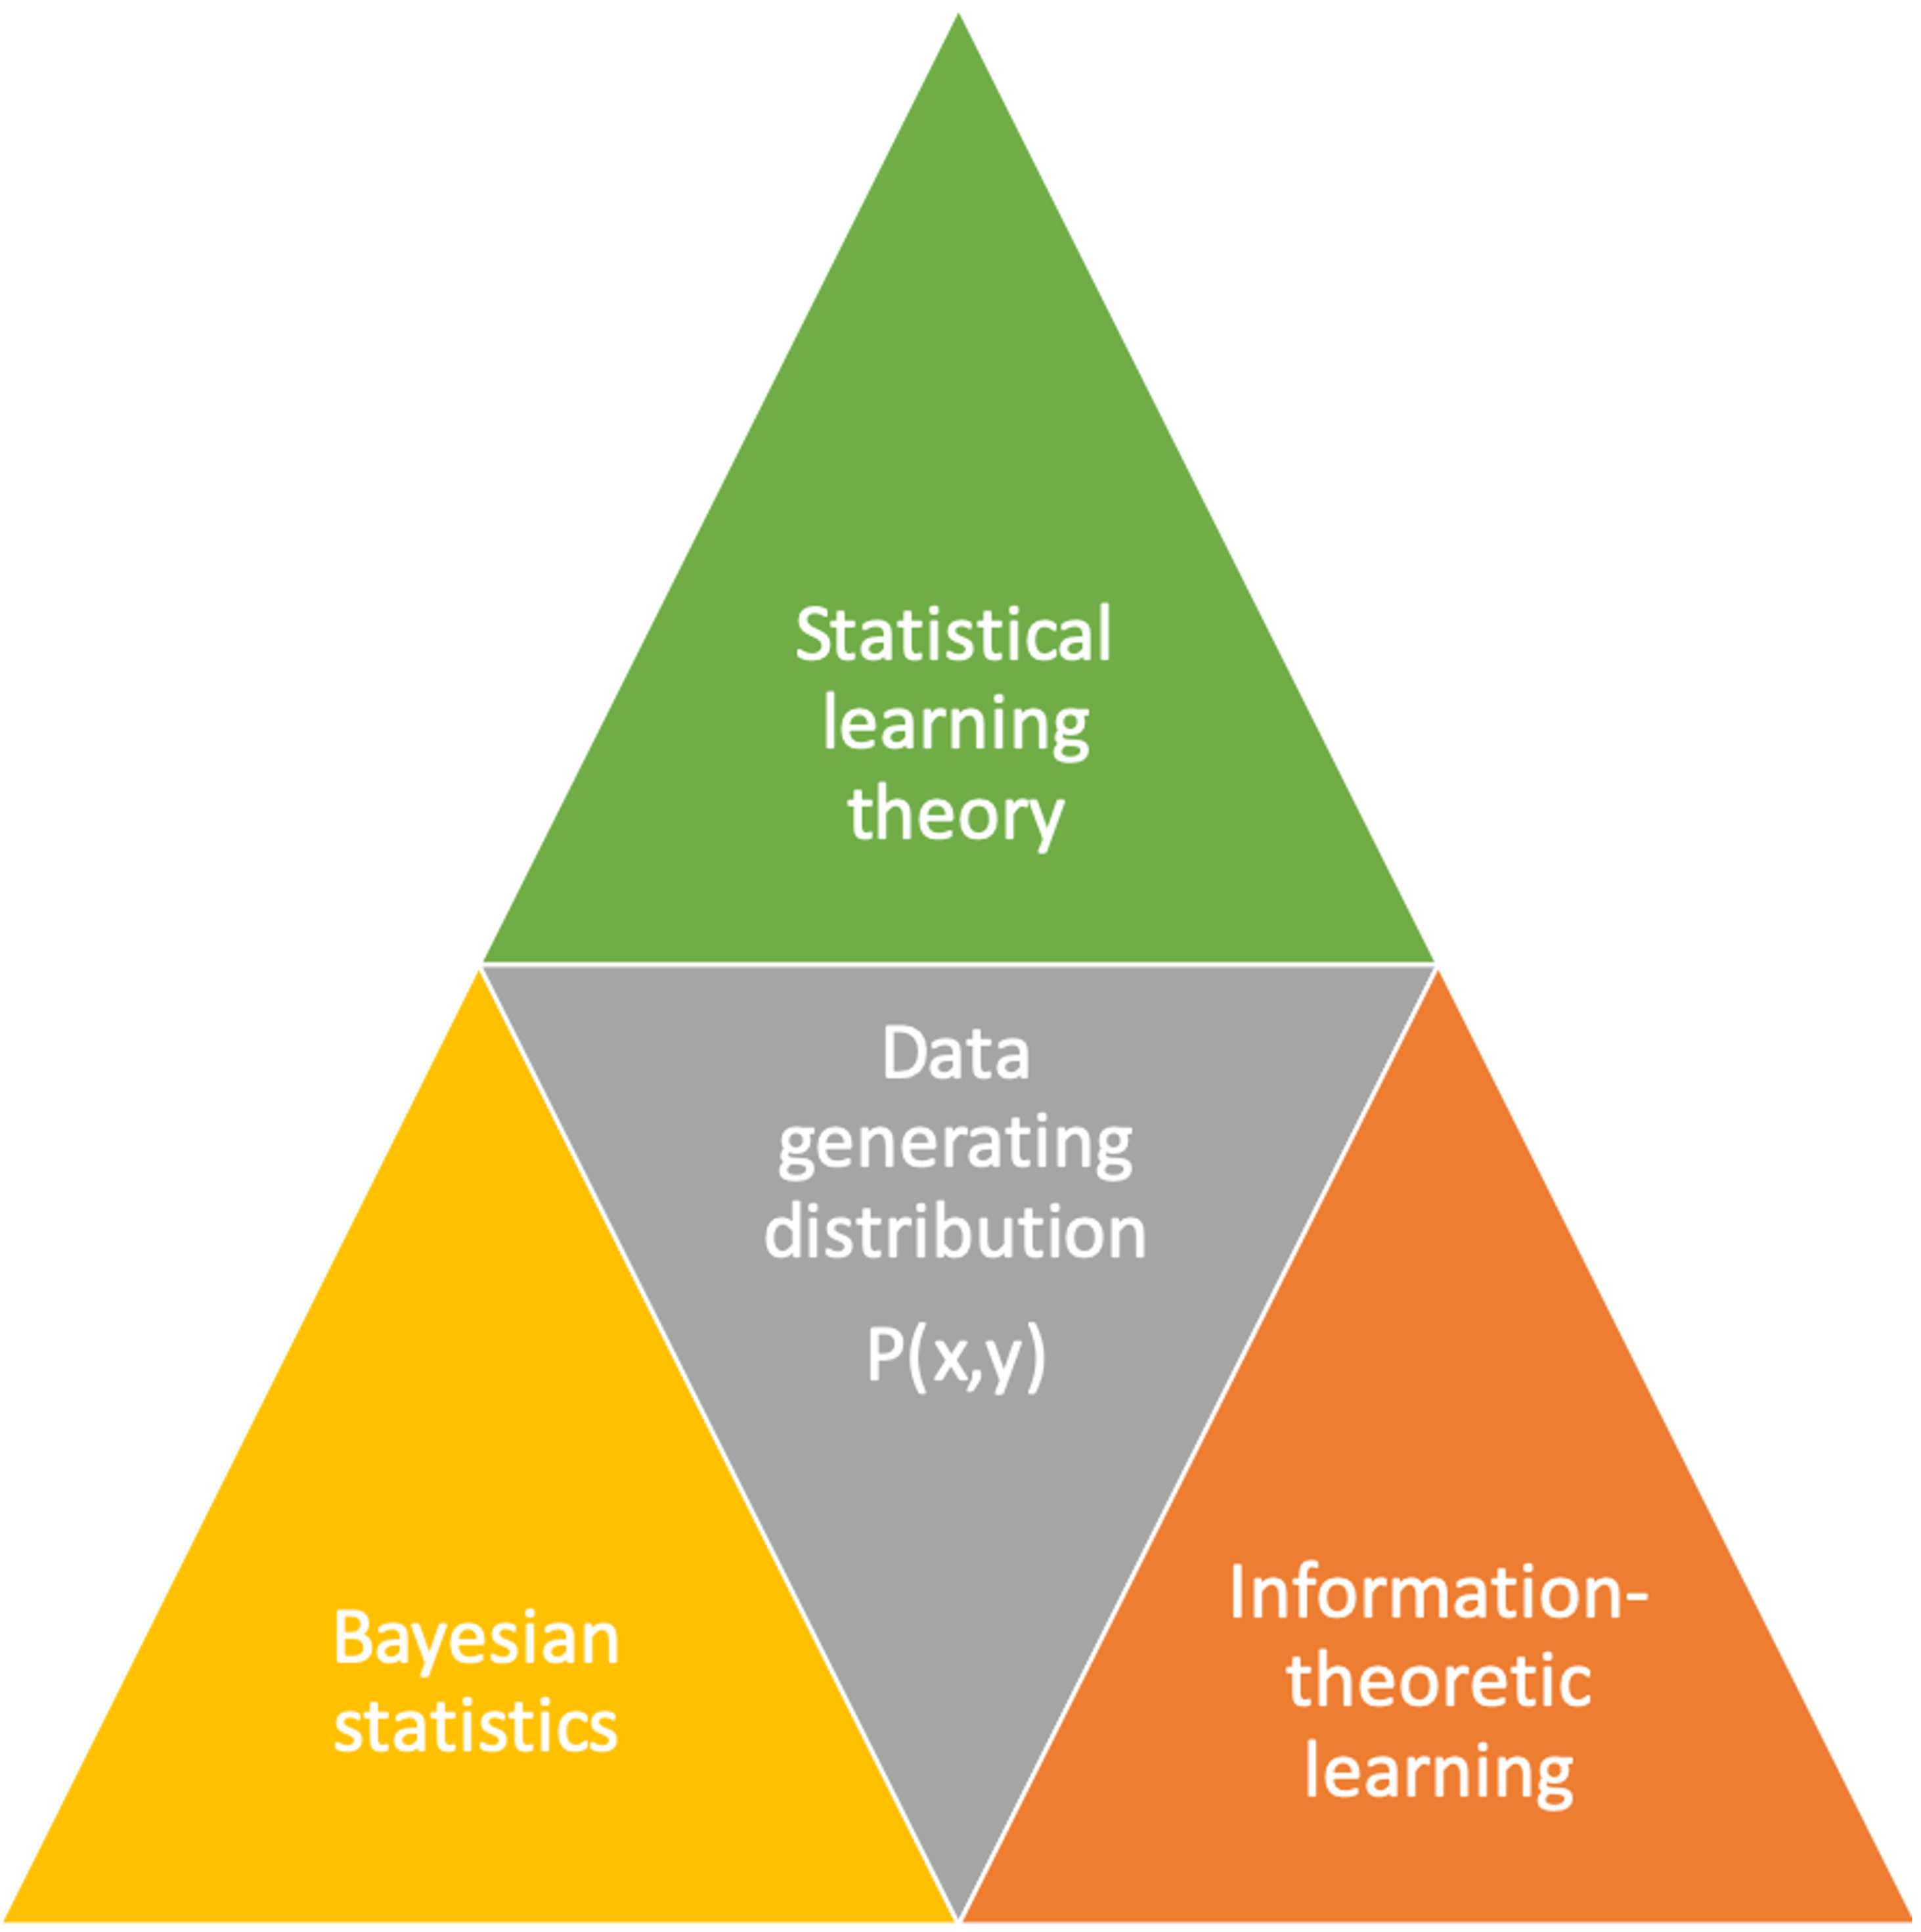
\includegraphics[width=0.4\columnwidth]{images/theoretical-paradigms.png}
    \caption{Paradigms for data generation distributions}
    \label{fig:fig1}
\end{figure}

\begin{itemize}
\item
  \textbf{\textcolor[HTML]{7EAA55}{Statistical learning theory (focus on this course)}:} assumes
  data is \uline{i.i.d} from an \uline{unknown distribution P(x)}, does not estimate the
  distribution (directly)
\item
  \textbf{\textcolor[HTML]{F5C342}{Bayesian Statistics}:} assumes \uline{prior information on P(x)}, estimates posterior probabilities
\item
  \textbf{\textcolor[HTML]{DE8344}{Information theoretic learning}:} (e.g.Minimum Description Length principle, MDL):
  estimates distributions, but does not assume a prior on P(x)

\end{itemize}

\subsection{Dimensions of a supervised learning algorithm
}\label{dimensions-of-a-supervised-learning-algorithm}

\begin{enumerate}
\def\labelenumi{\arabic{enumi}.}
\item
  \textbf{Training sample:} $S = \{(x_i, y_i)\}^m_{i=1}$ the training
  examples $(x, y) \in X \times Y$ independently drawn from a identical
  distribution $(i.i.d) D$ defined on $X \times Y, X$ is a space of inputs,
  $Y$ is the space of outputs.
\item
  \textbf{Model or hypothesis:} $h : X \rightarrow Y$ that we use to predict
  outputs given the inputs $x$.
\item
  \textbf{Loss function:} $L : Y \times Y \rightarrow \mathbb{R}, L(...) \geq 0, L(y, y')$ is the
  loss incurred when predicting $y'$ when $y$ is true.
\item
  \textbf{Optimization} procedure to find the hypothesis $h$ that
  minimize the loss on the training sample.
\end{enumerate}



\subsection{Classification (Task 1/3)}

\textbf{Problem:} partitioning the data into pre-defined classes by a
\emph{decision boundary} or \emph{decision surface}.

\textbf{Multi-class classification:} more than two classes

\begin{itemize}
  \item \textbf{Multi-label Classification:} An example can belong to multiple classes at the same time
  \item \textbf{Extreme classification:} Learning with thousands to hundreds of thousands of classes (Prof.~Rohit Babbar @ Aalto)
\end{itemize}



\subsubsection{Version space}\label{version-space}

\textbf{Version space:} the set of \uline{all \textcolor{blue}{consistent hypotheses}} of the
hypothesis class

\begin{itemize}
  \item
    \textbf{\textcolor{blue}{Consistent hypothesis}:} if correctly classifies all training
    examples
  \item
    \textbf{In version space:}
  \begin{itemize}
    \item
      \textbf{Most general hypothesis $G$:} cannot be expanded without
      including negative training examples
    \item
      \textbf{Most specific hypothesis $S$:} cannot be made smaller
      without excluding positive training points
  \end{itemize}
\end{itemize}

\begin{figure}[H]
  \centering  % Remember to centre the figure
    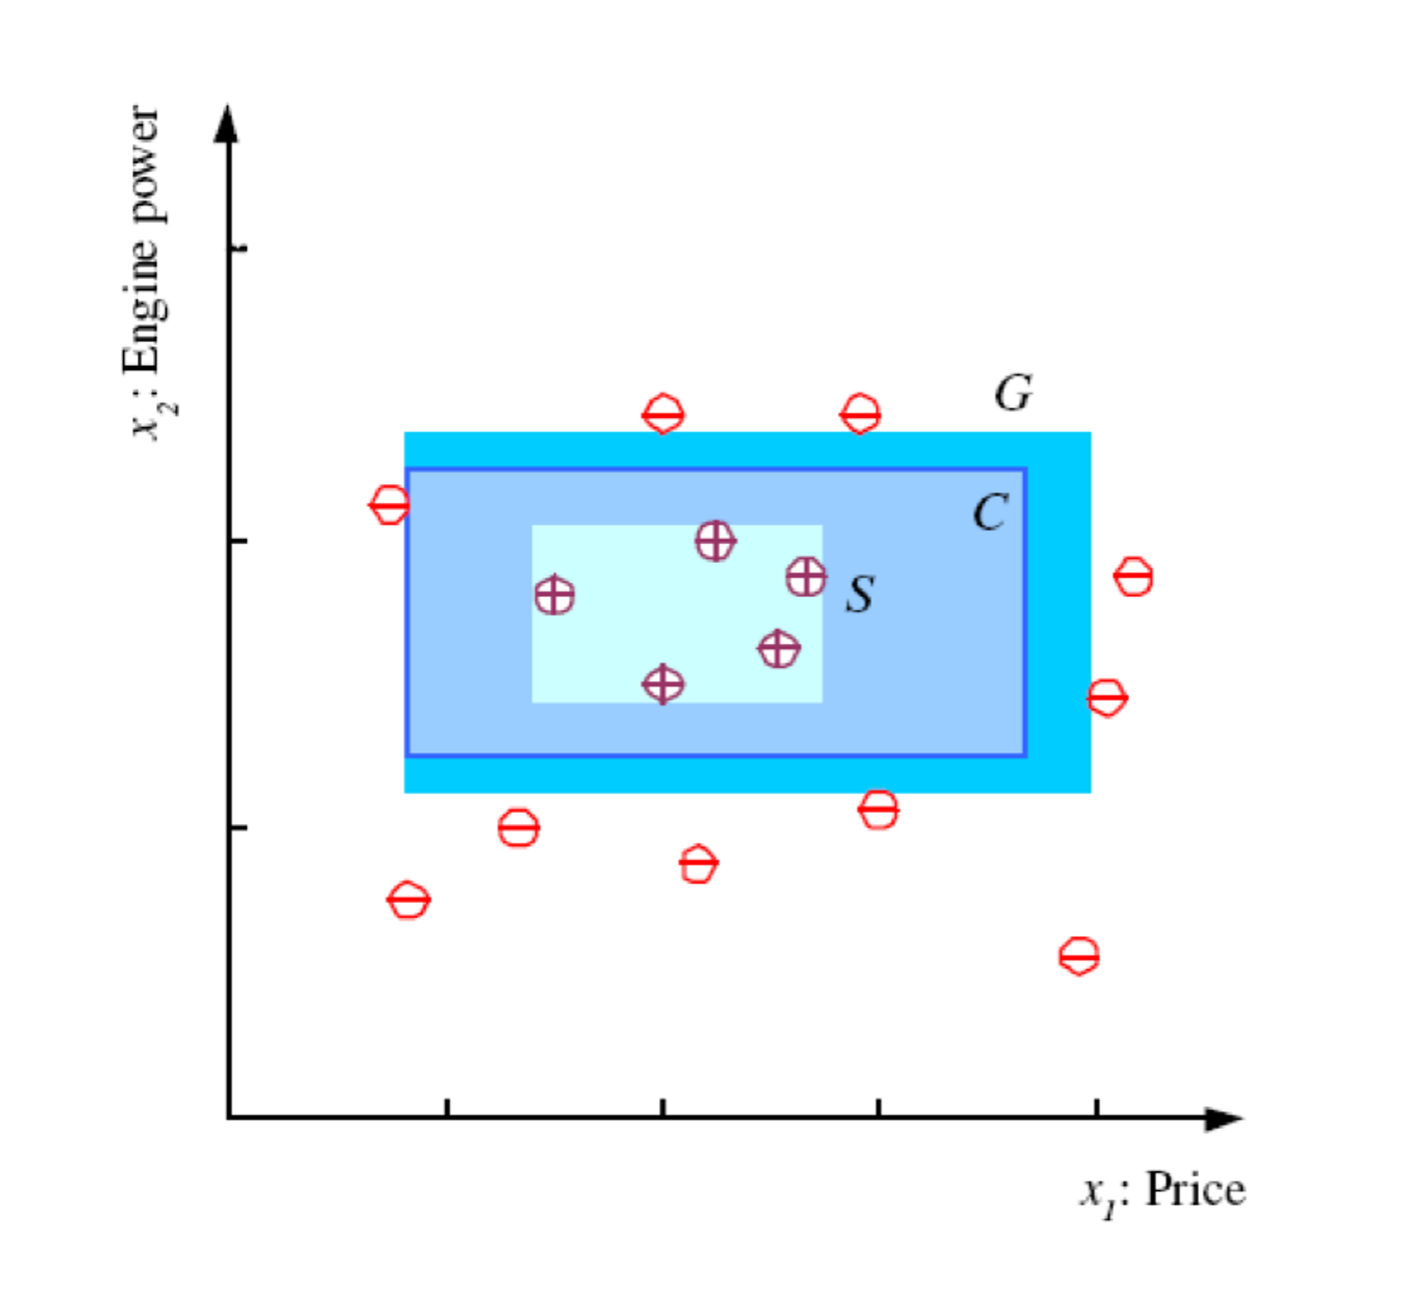
\includegraphics[width=0.5\columnwidth]{images/version-space.png}
    \caption{Illustration of a Version Space.}
    \label{fig:fig2}
\end{figure}

\begin{itemize}
\itemsep1pt\parskip0pt\parsep0pt
\item
  Intuitively, the \textbf{''safest'' hypothesis} to choose from the
  version space is the one that is furthers from the positive and
  negative training examples $\rightarrow$ maximum margin

  \begin{itemize}
  \itemsep1pt\parskip0pt\parsep0pt
  \item
    Margin = minimum distance between the decision boundary and a
    training point
  \end{itemize}
\end{itemize}






\subsection{Regression (Task 2/3) }\label{regression}

\textbf{Problem:} output variables which are numeric.





\subsection{Ranking \& preference learning (Task 3/3)
}\label{ranking-preference-learning}

\textbf{Problem:} predict a ordered list of preferred objects.

\textbf{Training data (typically):} pairwise preferences.

\begin{itemize}
  \item e.g.~user $x$ prefers movie $y_i$ over movie $y_j$
\end{itemize}

\textbf{Output:} ranked list of elements.




\subsection{Generalization}\label{generalization}

\textbf{Aim:} predict as well as possible the outputs of future
examples, not only for training sample.

We would like to \emph{minimize} the \textbf{generalization error}, or
the \textbf{(true) risk}:

\begin{equation} \label{eq:1}
  R(h) = E_{(x,y) \sim D}[L(h(x), y)]
\end{equation}
\begin{gather*}
  \textbf{Where:} \\
  \textbf{D}: \text{\uline{Unknown} distribution where from training and future} \\ \text{examples are drawn from (\uline{i.i.d assumption})}
\end{gather*}

\textbf{What can we say about $R(h)$} based on training examples and the
hypothesis class $\mathcal{H}$ alone? \uline{Two possibilities}:

\begin{itemize}
  \item Empirical evaluation by testing (Section \ref{model-evaluation-by-testing})
  \item Statistical learning theory (Section \ref{statistical-learning-theory})
\end{itemize}






\subsubsection{Model evaluation by testing
}\label{model-evaluation-by-testing}

\textbf{What:} estimate the model's ability to generalize on future data

\textbf{How:} approximating true risk by computing the
empirical risk on a independent test sample:

\[R_{test}(h) = \sum_{(x_i,y_i) \in S_{test}}^{m} L(h(x_i),y_i)\]

\begin{itemize}
  \item The expectation of $R_{test}(h)$ is the true risk $R(h)$
\end{itemize}




\subsection{Hypothesis classes }\label{hypothesis-classes}

There is a huge number of different \textbf{\textcolor{blue}{hypothesis classes}} or
\textbf{\textcolor{blue}{model families}} in machine learning, \textbf{e.g:}

\begin{itemize}
  \item
    \textbf{Linear models} such as logistic regression and perceptron
  \item
    \textbf{Neural networks:} compute non-linear input-output mappings
    through a network of simple computation units
  \item
    \textbf{Kernel methods:} implicitly compute non-linear mappings into
    high-dimensional feature spaces (e.g.~SVMs)
  \item
    \textbf{Ensemble methods:} combine simpler models into powerful
    combined models (e.g.~Random Forests)
\end{itemize}

Each have their different pros and cons in different dimensions
(accuracy, efficiency, interpretability); No single best hypothesis
class exists that would be superior to all others in all circumstances

\begin{center}\rule{3in}{0.4pt}\end{center}






\section{Statistical Learning Theory
}\label{statistical-learning-theory}

\textbf{What:} Statistical learning theory focuses in analyzing the generalization ability of learning algorithms. It's the theoretical background on machine learning.

\textbf{Goal:} Generalization (Section \ref{generalization})






\subsection{Probably Approximately Correct (PAC) learning
}\label{probably-approximately-correct-pac-learning}

\textbf{What:} The most studied \emph{theoretical framework} for \uline{analyzing the generalization performance} of machine learning algorithms. It formalizes the notion of generalization in machine learning. In practice, it's asking for bounding the generaliation error $(\epsilon)$ with high probability $(1 - \delta)$, with arbitrary level of error $\epsilon > 0$ and confidence $\delta > 0$.

\textbf{Ingredients:}

\begin{itemize}
  \item
    \textbf{input space $X$} containing all possible \textbf{inputs $x$}
  \item
    set of possible \textbf{labels $Y$} $($in binary
    classification $Y = \{0, 1\}$$)$
  \item
    \textbf{concept class $\mathcal{C}$} contains \textbf{concepts $C : X \rightarrow Y$} (to be learned),
    concept $C$ gives a label $C(x)$ for each input $x$
    \begin{itemize}
      \item \textcolor{Green}{underlying ground truth} $\rightarrow$ to be learn in the ideal case
      \item \textcolor{Red}{unknown in practice} (or otherwise ML is not needed)
    \end{itemize}
  \item Unknown (i.i.d) \textbf{probability distribution $D$} for the data
  \item \textbf{training sample $S = (x_1,C(x_1)),...,(x_m,C(x_m))$} drawn independently from $D$
  \item \textbf{hypothesis class $\mathcal{H}$}
  \begin{itemize}
    \item in the \textbf{basic case $\mathcal{H} = \mathcal{C}$} but this \colorbox{Yellow}{assumption can be relaxed}
  \end{itemize}
\end{itemize}

\textbf{Goal:} to learn a \uline{hypothesis with a low generalization error}. For 0/1 loss:

\[R(h) = E_{x \sim D} [L_{0/1}(h(x), C(x))] = Pr_{x \sim D} (h(x) \neq C(x))\]





\subsubsection{PAC learnability
}\label{pac-learnability}

\textbf{What:} Question, can we learn a concept class.

\bigskip \bigskip

\textbf{\textcolor{Green}{PAC-learnable}} concept class $\mathcal{C}$ if:

\begin{itemize}
  \item
     \uline{if there exist} an \textbf{algorithm $\mathcal{A}$} that given a training sample $S$ outputs a hypothesis $h_S \in \mathcal{H}$ that has generalization error satisfying
\end{itemize}

\begin{equation} \label{eq:2}
  Pr(\underbrace{R(\overbrace{h_S}^\text{chosen hypothesis from $\mathcal{H}$}) \leq \epsilon}_\text{"low generalization error" event}) \geq \underbrace{1 - \delta}_\text{success rate}
\end{equation}
\begin{gather*}
  P(GeneralizationError\;of\;h_S \leq GeneralizationError\;of\;interest) \geq Desired\;SuccessRate \\
  P(selection\;hypothesis\;(from \; \mathcal{H})\;with\;GeneralizationError \leq \epsilon) \geq Desired\;SuccessRate \\
  Probability\;of\;low\;GeneralizationError \geq Desired\;SuccessRate \\ \\
  \textbf{Where:} \\
  \textbf{$h_S$: } \text{output hypothesis} \\
  \textbf{$S$: } \text{training sample} \\
  \textbf{$m = |S|$: } \text{sample size that grows polynomially in $1/\epsilon$, $1/\delta$} \\
  \textbf{$\epsilon$: } \text{generalization error of interest (arbitrary)} \\
  \textbf{$1-\delta$: } \text{desired success rate / confidence (arbitrary)} \\
\end{gather*}


\textbf{\textcolor{Green}{Efficiently PAC-learnable}} concept class $\mathcal{C}$ if:

\begin{itemize}
  \item
     \textbf{\textcolor{Green}{PAC-learnable}}
   \item
      $\mathcal{A}$ runs in time polynomial in $m$, $1/\epsilon$, and $1/\delta$
      \begin{itemize}
        \item We want the \uline{requirement for training data} and \uline{running time} \textbf{not to explode} when we make $\epsilon$ and $\delta$ stricter $\rightarrow$ requirement of polynomial growth
      \end{itemize}
\end{itemize}


\textbf{Interpretation:}
\begin{itemize}
  \item $\epsilon$: sets the \uline{level of generalization error that is of interest} to us
  \begin{itemize}
    \item e.g. say we are satisfied with \textcolor{Red}{predicting incorrectly $10\%$} of the new datapoints $\rightarrow \epsilon = 0.10$
  \end{itemize}
  \item $1-\delta$: sets a \uline{level of confidence that is of interest} to us
  \begin{itemize}
    \item e.g. say we are satisfied of the \textcolor{Red}{training algorithm to fail $5\%$ of the time to provide a good hypothesis} $\rightarrow \delta = 0.05$
  \end{itemize}
  \item $\{R(h_S ) \leq \epsilon\}$: The \uline{event ”low generalization error”}
  \begin{itemize}
    \item considered as a \textit{random variable} because we cannot know beforehand which hypothesis $h_S \in \mathcal{H}$ will be selected by the algorithm
  \end{itemize}
\end{itemize}

\begin{figure}[H]
  \centering  % Remember to centre the figure
    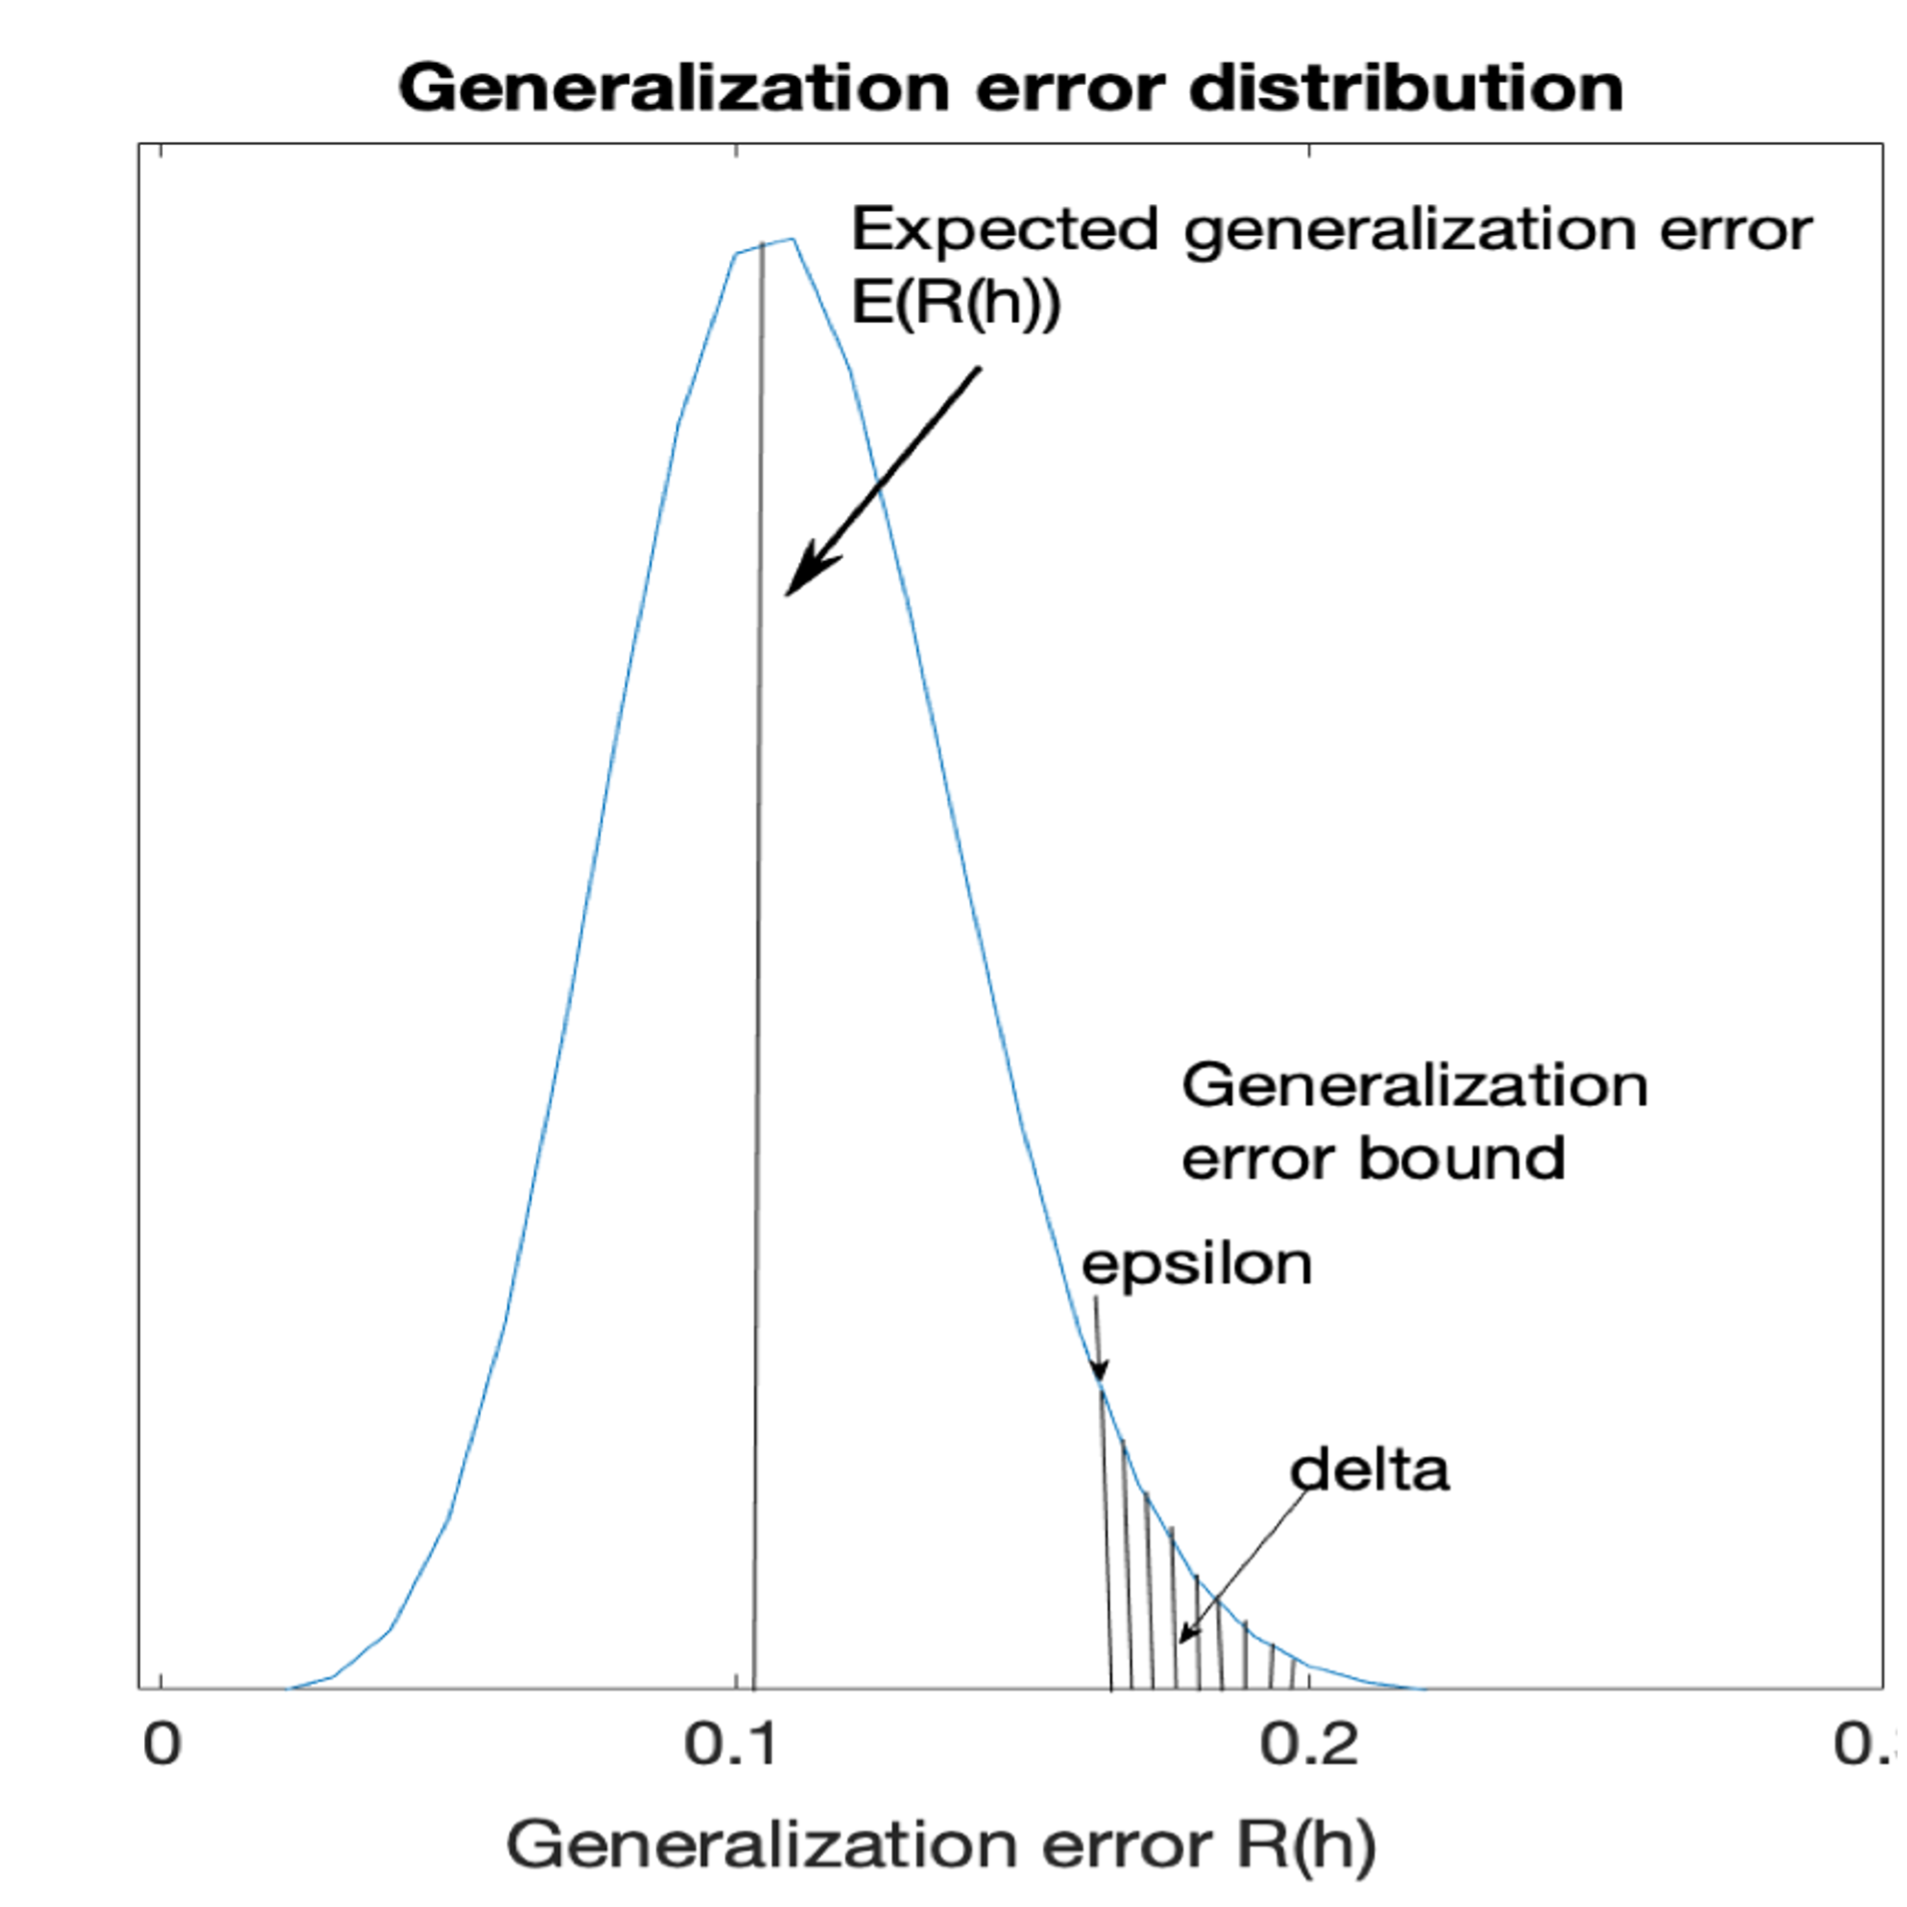
\includegraphics[width=0.6\columnwidth]{images/generalization-error-distribution.png}
    \caption{Generalization error distribution and error bound}
    \label{fig:fig3}
\end{figure}


\textbf{Generalization error bound vs. expected test error:}

\begin{itemize}
  \item We \uline{bound the probability of being in the high error tail} of the distribution (\uline{not the convergence to the mean or median generalization error}) $\rightarrow$ thus \textbf{empirically estimated test errors} might be considerably \uline{lower than the bounds suggest}.
\end{itemize}





\subsection{Learning with finite hypothesis classes
}\label{learning-with-finite-hypothesis-classes}

\textbf{What:} Finite concept classes arise when:

\begin{itemize}
  \item \textbf{Input variables} \uline{have finite domains} or they are converted to such in preprocessing (e.g. discretizing real values)
  \item The \uline{representations of the hypotheses have finite size} (e.g. the number of times a single variable can appear)
\end{itemize}

\bigskip \bigskip

\textbf{Finite hypothesis class - consistent case}

\begin{itemize}
  \item \textbf{Sample complexity bound} relying on the size of the hypothesis class (Mohri et al, 2018): $Pr(R(h_S) \leq \epsilon) \geq 1 - \delta$ if
  \[
  m \geq \frac{1}{\epsilon}(log(|\mathcal{H}|) + log(\frac{1}{\delta}))
  \]
  \item An equivalent \textbf{generalization error bound}:
  \[
  R(h) \leq \frac{1}{m}(log(|\mathcal{H}|) + log(\frac{1}{\delta}))
  \]
  \item \textbf{Holds for} \uline{any finite hypothesis class}
  \textbf{assuming there is a} \uline{consistent hypothesis}, \uline{one with zero empirical risk} \colorbox{Yellow}{or close to it (relaxed)}.
  \item The \uline{more hypotheses} there are in $\mathcal{H} \rightarrow$ the \uline{more training examples are needed}
\end{itemize}


\subsubsection{Example: Boolean conjunctions
}\label{example-boolean-conjunctions}


\textbf{What:} Example of a finity hypothesis class.

\bigskip \bigskip


\textbf{Example hypothesis class:} Boolean conjunctions

\begin{itemize}
  \item Dealing with subclasses of Boolean formulae, expressions \textbf{binary input variables} (literals) combined with \textbf{logical operators} \uline{AND} \& \uline{NOT}.
\end{itemize}

\bigskip \bigskip


\textbf{Example case:} Aldo likes to do sport only when the weather is suitable

\begin{itemize}
  \item \textbf{Training data:} Also has given examples of suitable and not suitable weather

  \begin{center}
    \begin{tabular}{ |c|c c c c c c|c| }
     \hline
      & \multicolumn{6}{|c|}{$x^t$} & $r(x^t)$ \\
       t & Sky & AirTemp & Humidity & Wind & Water & Forecast & EnjoySport \\
       \hline
       1 & Sunny & Warm & Normal & Strong & Warm & Same & 1 \\
       2 & Sunny & Warm & High & Strong & Warm & Same & 1 \\
       3 & Rainy & Cold & High & Strong & Warm & Change & 0 \\
       4 & Sunny & Warm & High & Strong & Cool & Change & 1 \\
       \multicolumn{8}{|c|}{} \\
       \multicolumn{8}{|c|}{\textcolor{blue}{Table:} Aldo's observed sport experiences in different weather conditions.} \\
     \hline
    \end{tabular}
  \end{center}

  \item \textbf{Model:} Let us build a classifier (boolean formulae containing AND, and NOT, but not OR operators) for Aldo to decide whether to do sports today
  \begin{itemize}
    \item e.g. if (Sky=Sunny) AND NOT (Wind=Strong) then (EnjoySport=1)
  \end{itemize}

  \item \textbf{Number of hypotheses $|\mathcal{H}|$:}
  \begin{itemize}
    \item \textbf{Each variable:} "AND", "AND NOT", or can be excluded from the rule $\rightarrow$ \uline{3 possibilities}
    \item \textbf{Total number of hypotheses} is thus $3^d$, where d is the number of variables $\rightarrow |\mathcal{H}| = 3^6 = \uline{729}$
  \end{itemize}

  \item \textbf{Plotting the bound for Aldo’s problem using boolean conjunctions:}
  \begin{itemize}
    \item \textbf{Left plot:} generalization bound $\epsilon$ is shown for different values of delta $\delta$, using d = 6 variables.
    \item \textbf{Right plot:} generalization bound $\epsilon$ is shown for increasing number of input variables d, using delta $\delta = 0.05$

    \begin{figure}[H]
      \centering  % Remember to centre the figure
        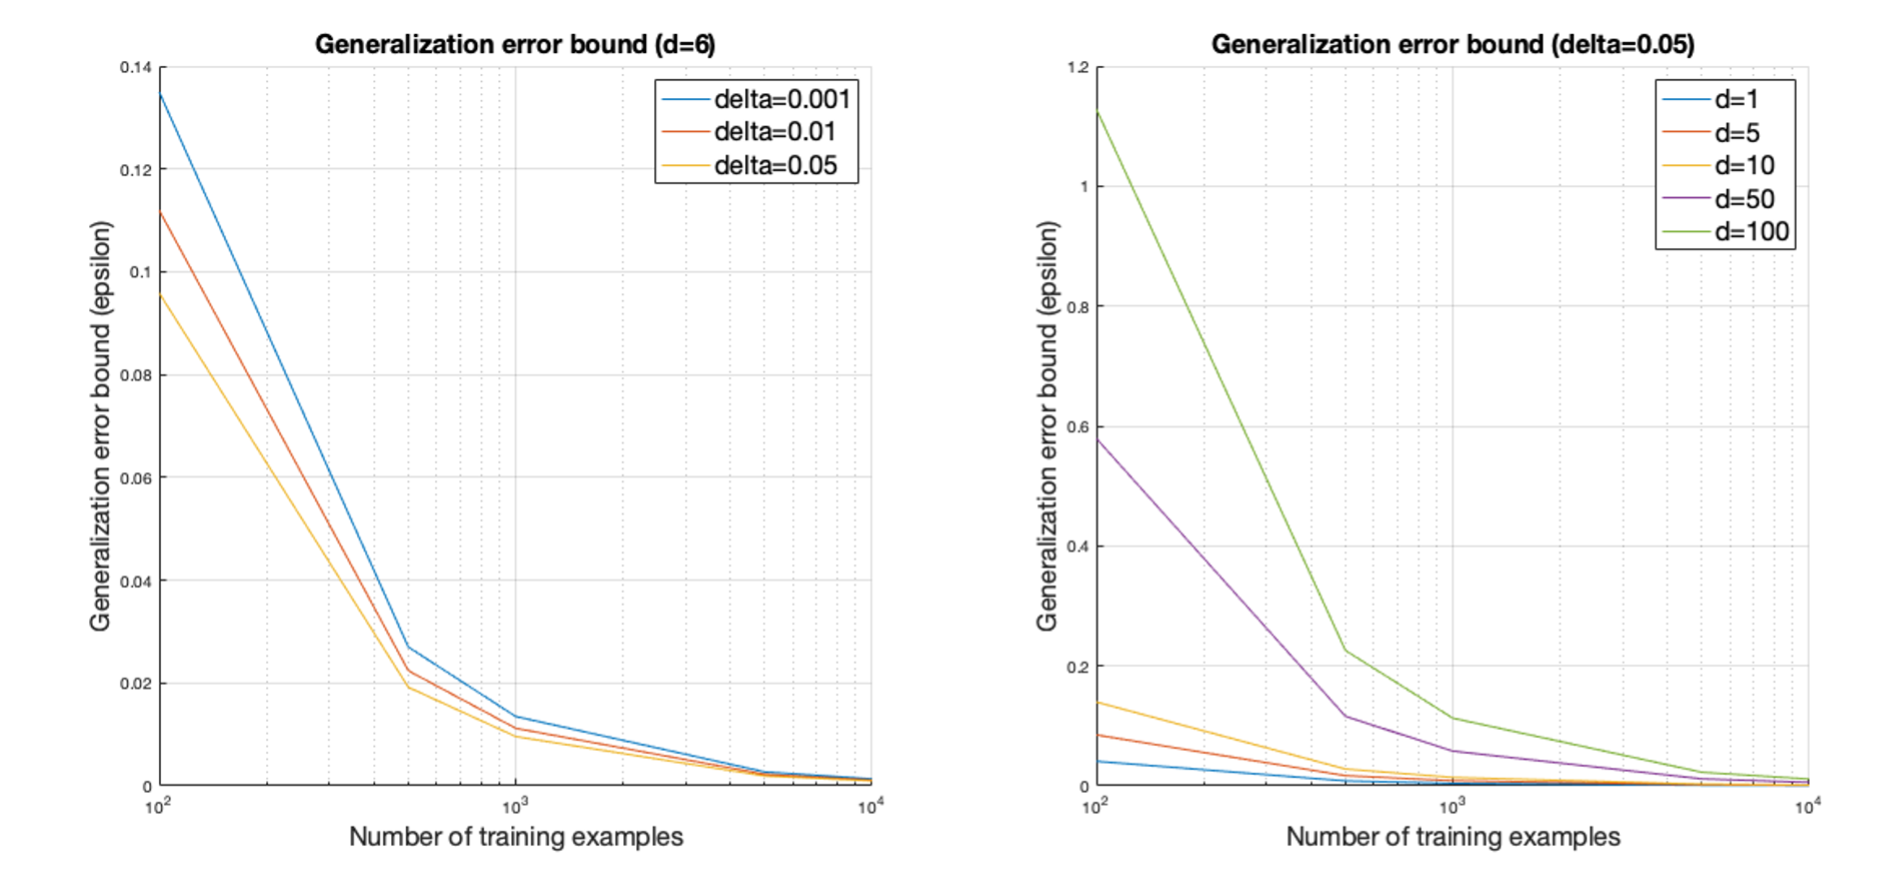
\includegraphics[width=1.0\columnwidth]{images/eg1-generalization-error-bound.png}
        \caption{Boolean conjunctions: Generalization error bounds}
        \label{fig:fig4}
    \end{figure}

  \end{itemize}

  \item \textbf{Typical behaviour of ML learning algorithms is revealed:}
  \begin{itemize}
    \item \textbf{\textcolor{Green}{increase of sample size decreases generalization error}}
    \item extra data gives \textbf{\textcolor{Red}{less and less additional benefit as the sample size grows}} (law of diminishing returns)
    \item requiring high level of confidence (small $\delta$) for obtaining low error requires more data for the same level of error
  \end{itemize}

\end{itemize}






\subsection{Learning with infinite hypothesis classes
}\label{learning-with-infinite-hypothesis-classes}


Most models used in practise rely on infinite hypothesis classes, e.g.

\begin{itemize}
  \item $\mathcal{H}$ = hyperplanes in $\mathbb{R}^d$ (e.g. Support vector machines)
  \item $\mathcal{H}$ = neural networks with continuous input variables
\end{itemize}





\subsubsection{Vapnik-Chervonenkis (VC) dimension}\label{vapnik-chervonenkis-dimension}

\textbf{Purpose:} Vapnik-Chervonenkis dimension lets us \textbf{study} \uline{learnability of infinite hypothesis classes} \textbf{through} the concept of \uline{\textcolor{Purple}{shattering}}

\textbf{What:} can be understood as measuring the \uline{capacity of a hypothesis class to adapt to different concepts}

\begin{itemize}
  \item $VCdim(\mathcal{H}) =$ \uline{size} of the \textbf{largest training set} that we can find a \textbf{consistent classifier for all labelings in $Y^m$}
  \item Intuitively:
  \begin{itemize}
    \item low $VCdim \rightarrow$ easy to learn, low sample complexity
    \item high $VCdim \rightarrow$ hard to learn, high sample complexity
    \item infinite $VCdim \rightarrow$ cannot learn in PAC framework
  \end{itemize}
\end{itemize}

\bigskip \bigskip

\textbf{How to show that $VCdim(\mathcal{H}) = d$ for a hypothesis class:}
\begin{itemize}
  \item We need to show two facts:
  \begin{enumerate}
    \item There \textcolor{Green}{exists} a \uline{set of inputs of size $d$ that \textbf{can be \textcolor{Purple}{shattered}} by hypothesis in $\mathcal{H}$} (i.e. we can pick the set of inputs any way we like): $VCdim(\mathcal{H}) \geq d$
    \item There \textcolor{Red}{does not exist} any \uline{set of inputs of size $d + 1$ that \textbf{can be \textcolor{Purple}{shattered}}} (i.e. need to show a general property): $VCdim(\mathcal{H}) < d + 1$
  \end{enumerate}
\end{itemize}

\bigskip \bigskip

\textbf{Formally:} (for binary labelings)

\begin{itemize}
  \item Through \textbf{growth function}:
    $$
    \sqcap_{\mathcal{H}}(m) = \max_{ \{x_1, ..., x_m\} \subset X } |\{(h(x_1), ..., h(x_m)) : h \in \mathcal{H}\}|
    $$
    \begin{itemize}
      \item The growth function gives the \uline{maximum number of unique labelings} the hypothesis class $\mathcal{H}$ can provide for an arbitrary set of input points
      \item The maximum of the growth function is \uline{$2^m$ for a set of $m$ examples}
    \end{itemize}
    \item \textbf{Vapnik-Chervonenkis dimension} is then
    $$
    VCdim(\mathcal{H}) = \max_{m}\{m | \sqcap_{\mathcal{H}}(m) = 2^m\}
    $$
\end{itemize}





\subsubsubsection{Shattering}\label{shattering}

\textbf{What:} underlying concept in VC dimension

\textbf{Given:} a set of points $S = {x_1,...,x_m}$ and a fixed class of functions $\mathcal{H}$

\textbf{$\mathcal{H}$ is said to \textcolor{Purple}{shatter} $S$ if:} for any possible partition of $S$ into positive $S_+$ and negative subset $S_-$ we can find a hypothesis for which $h(x) = 1$ if and only if $x \in S_+$

\begin{figure}[H]
  \centering  % Remember to centre the figure
    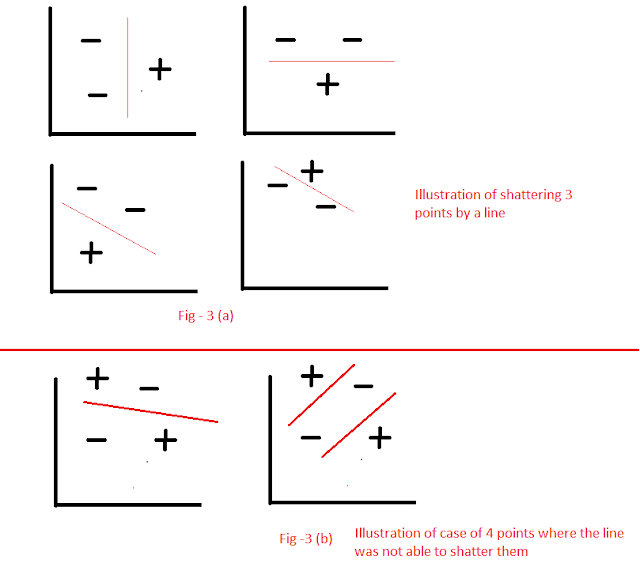
\includegraphics[width=0.9\columnwidth]{images/shattering.png}
    \caption{Illustration of shattering}
    \label{fig:fig5}
\end{figure}





\subsubsubsection{Generalization bound with VC-dimension}\label{deneralization-bound-with-vc-dimension}

\textbf{What:} Way of using VC-dimensions to analyze machine learning algorithms.

(Mohri, 2018) Let $\mathcal{H}$ be a family of functions taking values in ${-1, +1}$ with VC-dimension $d$ . Then for any $\delta > 0$, with probability at least $1 - \delta$ the following holds for all $h \in \mathcal{H}$:

$$
R(h) = \underbrace{\hat{R}(h)}_\text{empirical risk} + \sqrt{\frac{2\log{(em/d)}}{m/d}} + \sqrt{\frac{\log{(1/\delta)}}{2m}}
$$

\begin{gather*}
  \textbf{Where:} \\
  \textbf{$d$: } \text{VC-dimension} \\
  \textbf{$m$: } \text{amount of training data} \\
  \textbf{$e$: } \text{Euler's number, $e \approx 2.71828$} \\
  \textbf{$\delta$: } \text{failure rate} \\
\end{gather*}

\begin{itemize}
  \item $m/d$ shows that changing to a model with higher VC-dimension $d$ makes the same amount of training samples $m$ less effective. $\rightarrow$ the second term grows when VC-dimension grows.
  \begin{itemize}
    \item For more complex $\mathcal{H}$ class, one needs more data $m$ to guarantee similar kind of generalization.
  \end{itemize}
  \item Manifestation of the \textbf{Occam’s razor principle:} to justify an increase in the complexity, we need reciprocally more data
\end{itemize}




\subsubsection{Rademacher complexity}\label{rademacher-complexity}


\textbf{What:} Rademacher complexity defines complexity as the capacity of hypothesis class to fit random noise

\textbf{Why:} Rademacher complexity is a practical alternative to VC dimension, giving typically sharper bounds (but requires a lot of simulations to be run).


\bigskip \bigskip


\textbf{Experiment:} how well does your hypothesis class fit noise?

\begin{itemize}
  \item Consider a \textbf{set of training examples $S_0 = \{(x_i , y_i)\}^m_{i=1}$}
  \item \textbf{Generate $M$ new datasets $S_1 , ... , S_M$} from $S_0$ by randomly drawing a new label $\sigma \in Y$ for each training example in $S_0$
  $$
  S_k = \{(x_i, \sigma_{ik})\}^m_{i=1}
  $$
  \item Train a classifier $h_k$ minimizing the empirical risk on training set $S_k$, record its empirical risk
  $$
  \hat{R}(h_k) = \frac{1}{m} \sum_{i=1}^{m} 1_{h_k(x_i) \neq \sigma_{ik}}
  $$
  \item \textbf{Compute the average empirical risk over all datasets:}
  $$
  \bar{\epsilon} = \frac{1}{M} \sum_{k=1}^{M} \hat{R}(h_k)
  $$
  \item \textbf{Observe the quantity:}
  $$
  \hat{\mathcal{R}} = \frac{1}{2} - \bar{\epsilon}
  $$
  \begin{itemize}
    \item When ($\hat{\mathcal{R}} = 0, \bar{\epsilon} = 0.5$) $\rightarrow$ predictions correspond to random coin flips (0.5 probability to predict either class)
    \item When ($\hat{\mathcal{R}} = 0.5, \bar{\epsilon} = 0$) $\rightarrow$ all hypotheses $h_i , i = 1, ... , M$ have zero empirical error (perfect fit to noise, not good!)
    \item \textbf{Ideally we want:}
    \begin{itemize}
      \item to be able to \textbf{\textcolor{Green}{separate noise from signal}}
      \begin{itemize}
        \item Meaning large $\bar{\epsilon}$, so that the model is bad at classifying random noise. $\rightarrow$ low complexity $\hat{\mathcal{R}}$.
      \end{itemize}
      \item to have \textbf{\textcolor{Green}{low empirical error on real data}} - otherwise impossible to obtain low generalization error
    \end{itemize}
  \end{itemize}
\end{itemize}



\textbf{Rademacher complexity:}

\begin{itemize}
  \item For binary classification with labels $Y = \{-1, +1\}$ \textbf{empirical Rademacher complexity} can be defined as
  $$
  \hat{\mathcal{R}}_S(\mathcal{H}) = \frac{1}{2} E_\sigma (\underbrace{\sup_{h \in \mathcal{H}} \frac{1}{m} \sum_{t=1}^m \overbrace{\sigma^i}^\text{random true label } \overbrace{h(x_i)}^\text{ predicted random label}}_\text{hypothesis with highest correlation with random label})
  $$
  \begin{gather*}
    \textbf{Where:} \\
    \textbf{$\sigma_i \in \{-1, +1\}$: } \text{are Rademacher random variables,} \\
    \text{drawn independently from uniform distribution}  \\
    \text{(i.e. $Pr\{\sigma = 1\} = 0.5)$} \\
  \end{gather*}
  \item We can also rewrite \textbf{$\hat{\mathcal{R}}_S$ in terms of empirical error}
  $$
  \hat{\mathcal{R}}_S = \frac{1}{2} - E_\sigma \inf_{h \in \mathcal{H}} \hat{\epsilon}(h)
  $$
  \begin{itemize}
    \item Now we have Rademacher complexity in terms of \uline{expected minimum error of classifying randomly labeled data}
  \end{itemize}
\end{itemize}





\subsubsubsection{Generalization bound with Rademacher complexity}\label{deneralization-bound-with-rademacher-complexity}

(Mohri et al. 2018): For any $\delta > 0$, with probability at least $1 - \delta$ over a sample drawn from an unknown distribution $D$, for any $h \in \mathcal{H}$ we have:

$$
R(h) \leq \underbrace{\hat{R}_S(h)}_\text{empirical risk} + \underbrace{\hat{\mathcal{R}}_S(\mathcal{H})}_\text{empirical Rademacher complexity} + 3 \sqrt{\frac{\log{\frac{2}{\delta}}}{2m}}
$$





\subsubsection{Vapnik-Chervonenkis dimension VS. Rademacher complexity}\label{vapnik-chervonenkis-dimension-vs-rademacher-complexity}

Note the differences between Rademacher complexity and VC dimension

\begin{itemize}
  \item Dependency on training data
  \begin{itemize}
    \item \textbf{VC dimension:} \uline{independent} $\rightarrow$ measures the \textcolor{Red}{worst-case} where the data is generated in a bad way for the learner
    \item \textbf{Rademacher complexity:} \uline{depends on the training sample} thus is dependent on the data generating distribution
  \end{itemize}
  \item Focus
  \begin{itemize}
    \item \textbf{VC dimension:} extreme case of realizing all labelings of the data
    \item \textbf{Rademacher complexity:} measures smoothly the ability to realize random labelings
  \end{itemize}
\end{itemize}


\bigskip \bigskip


Example: Rademacher and VC bounds on a real dataset


\begin{figure}[H]
  \centering  % Remember to centre the figure
    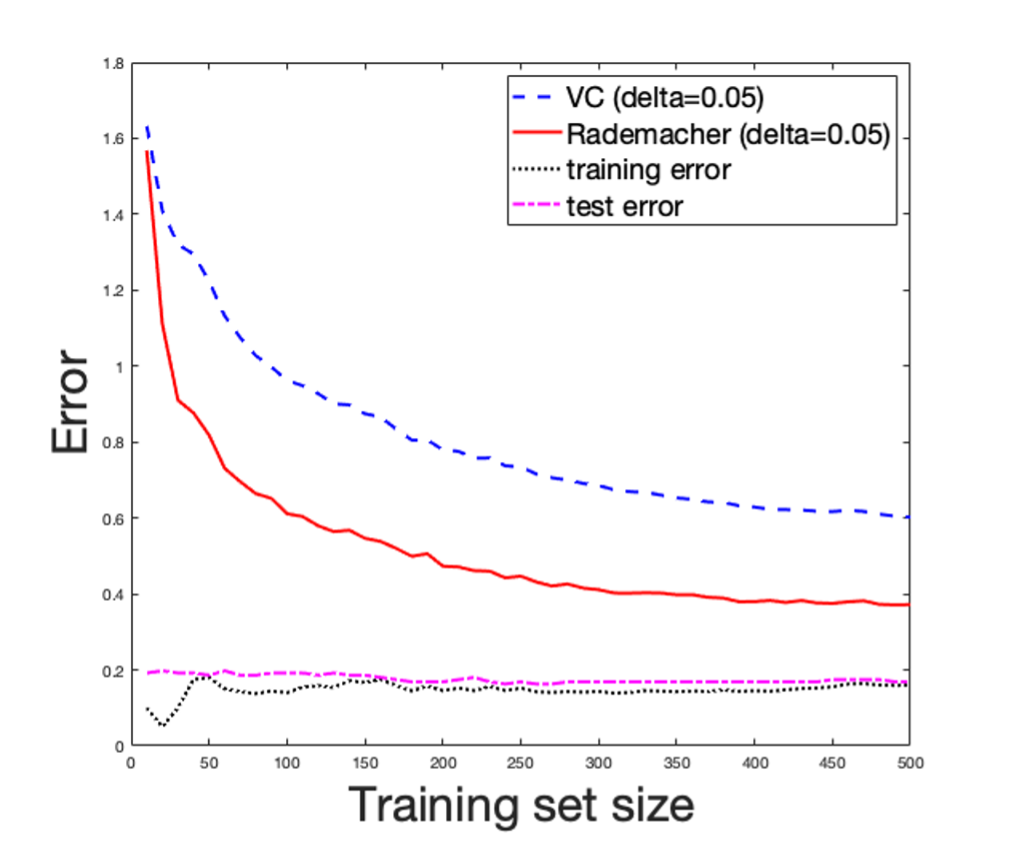
\includegraphics[width=0.7\columnwidth]{images/rademacher-vs-vc.png}
    \caption{Rademacher and VC bounds on a real dataset}
    \label{fig:fig6}
\end{figure}

\begin{itemize}
  \item Rademacher bound is sharper than the VC bound
  \item VC bound is not yet informative with 500 examples $(> 0.5)$ using $(\delta = 0.05)$
  \item The gap between the mean of the error distribution ($\approx$ test error) and the 0.05 probability tail (VC and Rademacher bounds) is evident (and expected)
\end{itemize}


\begin{center}\rule{3in}{0.4pt}\end{center}


















\section{Model selection}\label{model-selection}

\textbf{Key principle:} Model selection in machine learning can be seen to implement Occam’s razor:

\begin{itemize}
  \item \textbf{Occam's razor, (principle of parsimony)} is the \textit{problem-solving principle} that "\uline{entities should not be multiplied beyond necessity}".
  \item \textbf{Simply:} \uline{If there are several equally correct explanations} for some phenomenon, the \uline{simplest explanation is the most preferred one}.
  \begin{figure}[H]
    \centering  % Remember to centre the figure
      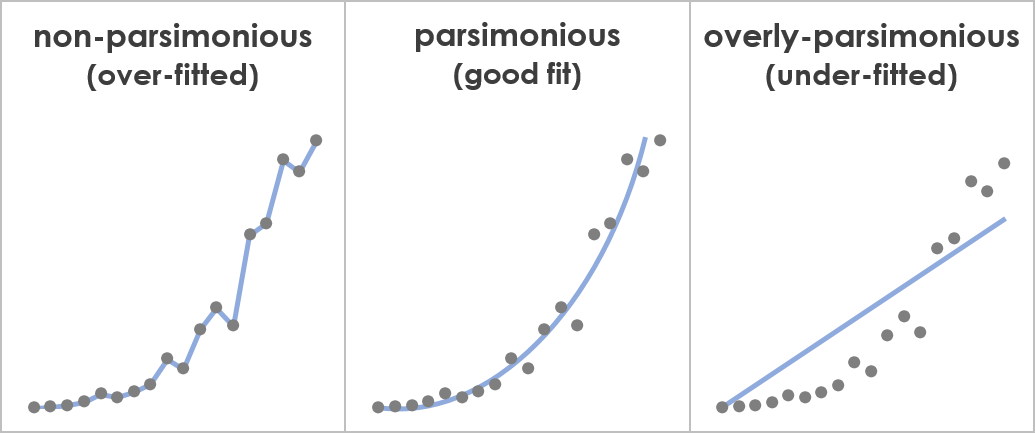
\includegraphics[width=0.6\columnwidth]{images/eg-of-parsimony.png}
      \caption{Illustration of parsimony in the context of ML models}
      \label{fig:eg-of-parsimony}
  \end{figure}
  \item \textbf{In model selection:} captures the \textcolor{Purple}{trade-off between} \uline{generalization error (bias \& variance)} and \uline{model complexity}.
  \begin{figure}[H]
    \centering  % Remember to centre the figure
      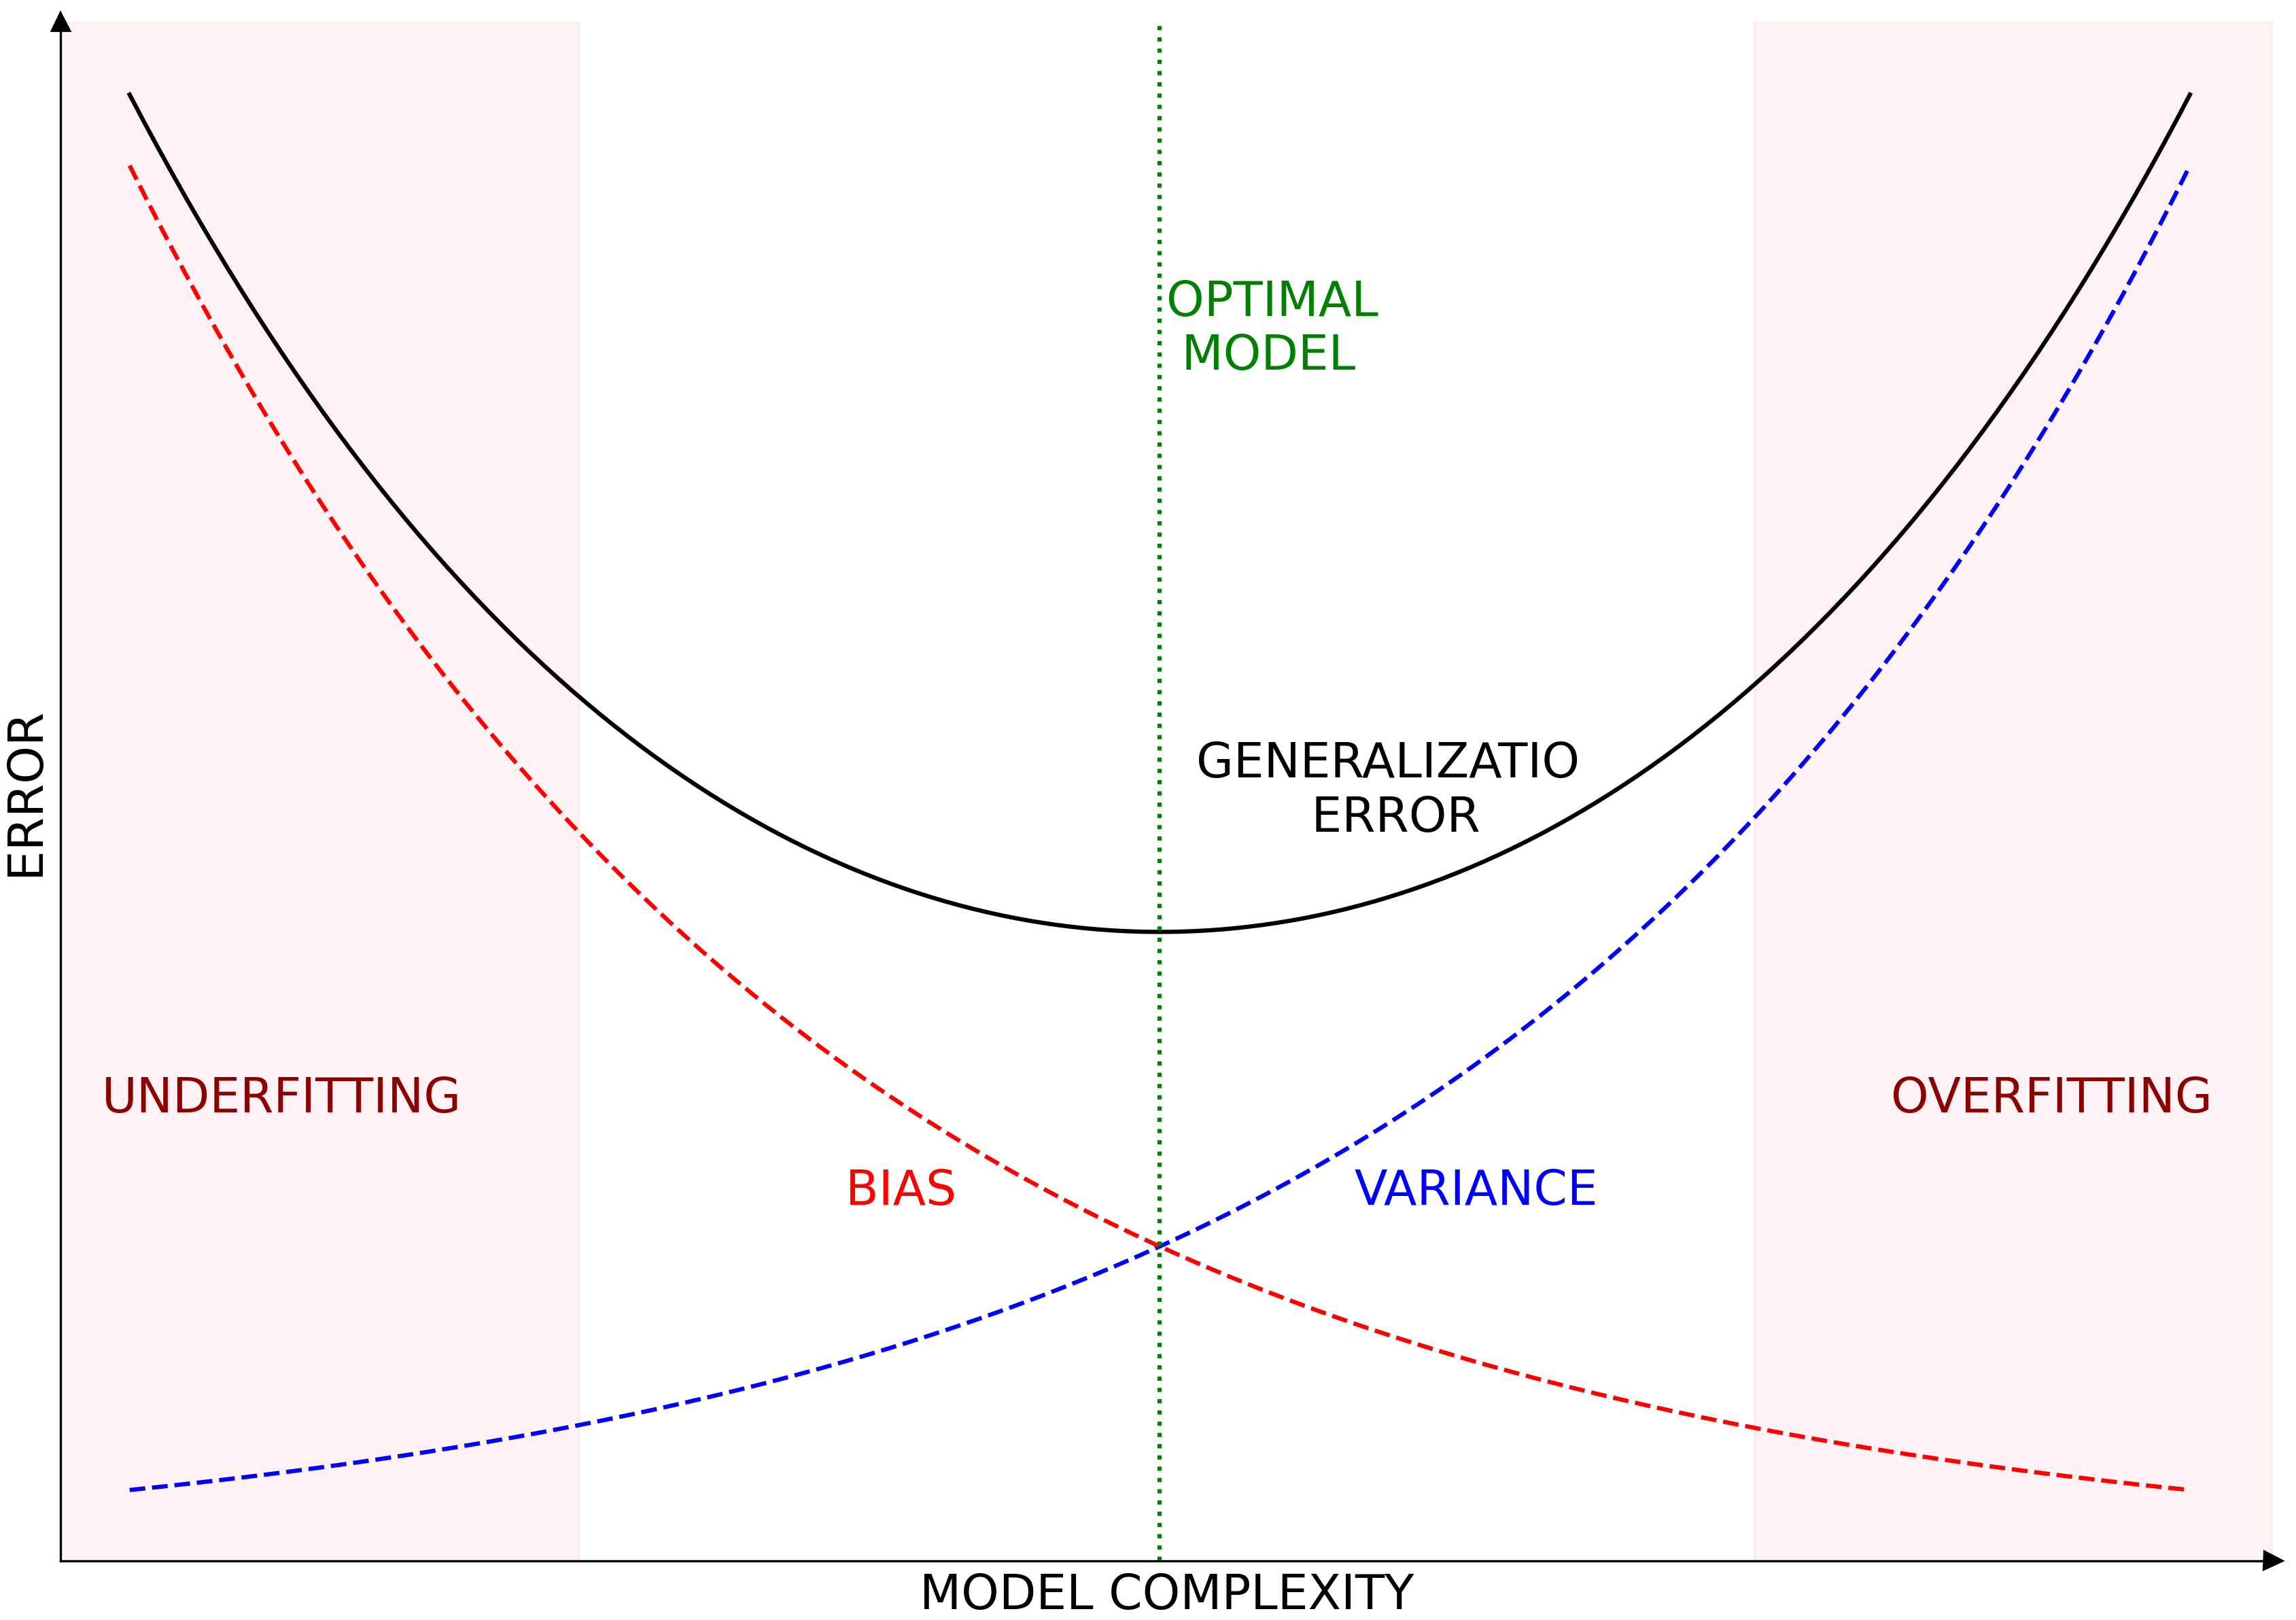
\includegraphics[width=0.7\columnwidth]{images/bias-variance-tradeoff.png}
      \caption{Illustration of parsimony in the context of ML models}
      \label{fig:bias-variance-tradeoff}
  \end{figure}
\end{itemize}


\textbf{Scenario – what we assume from the data:}
\begin{itemize}
  \item \textbf{So far- DETERMINISTIC SCENARIO:} The analysis so far assumed that the \uline{labels are \textcolor{blue}{deterministic functions} of the input}
  \item \textbf{Now- STOCHASTIC SCENARIO:} Relaxes this assumption by assuming the \uline{output is a \textcolor{blue}{probabilistic function} of the input}
  \begin{itemize}
    \item Inputs $X$ and outputs $Y$ are generated by a joint probability distribution $D$ or $X \times Y$
    \item In the stochastic scenario, there \textbf{may not always exist a target concept $f$} that has zero generalization error $R(f) = 0$
  \end{itemize}
\end{itemize}


\textbf{Sources of stochasticity:} stochastic dependency between input and output can arise from various sources
\begin{itemize}
  \item \textcolor{red}{Imprecision} in recording the \uline{input data} (e.g. measurement error), shifting our examples
  \item \textcolor{red}{Errors} in the \uline{labeling} of the training data (e.g. human annotation errors), flipping the labels some examples
  \item There may be \textcolor{red}{additional variables} that affect the labels that are \uline{not part of our input data}
\end{itemize}
\uline{All of these sources of stochasticity} could be characterized as adding \textbf{noise} (or \textbf{hiding signal})


\textbf{NOISE (All sources of stochasticity) and Complexity:}
\begin{itemize}
  \item \textbf{Typical effect:} make the decision boundary \uline{more complex} (e.g. a spline curve instead of a hyperplane). But this \textcolor{red}{may not give a better generalization error}, \textbf{if} we end up merely \uline{re-classifying points corrupted by noise}.
  \item In practice, we need to \textbf{balance} the \uline{complexity} of the hypothesis and the \uline{empirical error} carefully
  \begin{itemize}
    \item A \textbf{too simple model} \textcolor{red}{does not allow optimal empirical error to obtained}, this is called underfitting
    \item A \textbf{too complex model} may obtain zero empirical error, but have \textcolor{red}{worse than optimal generalization error}, this is called overfitting
    \begin{figure}[H]
      \centering  % Remember to centre the figure
        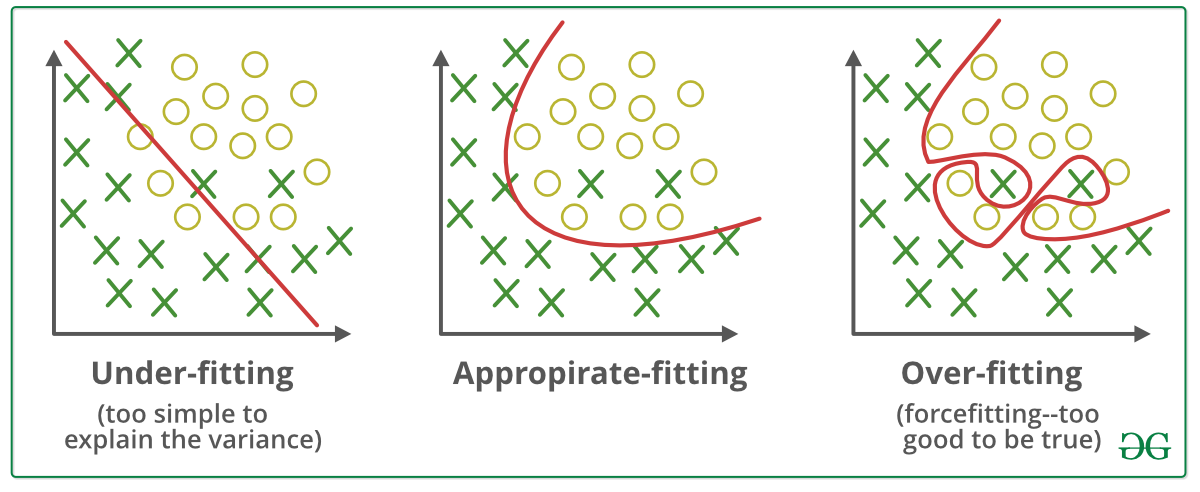
\includegraphics[width=0.8\columnwidth]{images/underfit-appropriate-overfit.png}
        \caption{Illustration of under- and overfitting}
        \label{fig:underfit-appropriate-overfit}
    \end{figure}
  \end{itemize}
\end{itemize}


\textbf{Controlling complexity (2 general approaches):}
\begin{enumerate}
  \item \textbf{Hypothesis Class selection:} e.g. the maximum degree of polynomial to fit the regression model
  \item \textbf{Regularization:} penalizing the use of too many parameters
\end{enumerate}



\textbf{Measuring complexity}

\begin{itemize}
  \item We have already looked at some measures:
  \begin{itemize}
    \item \textbf{Number of distinct hypotheses $|\mathcal{H}|$:} works for finite $\mathcal{H}$
    \item \textbf{Vapnik-Chervonenkis dimension (VCdim) (Section \ref{vapnik-chervonenkis-dimension}):} the maximum number of examples that can be classified in all possible ways by choosing different hypotheses $h \in \mathcal{H}$
    \item \textbf{Rademacher complexity (Section \ref{rademacher-complexity}):} measures the capability to classify after randomizing the labels
  \end{itemize}
  \item Lots of other complexity measures and model selection methods exist (not in the scope here)
\end{itemize}















\subsection{Bayes error}\label{bayes-error}

\textbf{Bayes error} is the \uline{minimum achievable error} (non-zero), given a distribution $D$ over $X \times Y$ (\textit{stochastic scenario}), by measurable functions $h: X \rightarrow Y$

$$
R^* = \inf_{\{h | h\;measurable\}} R(h)
$$

\begin{itemize}
  \item Note that we cannot actually compute $R^* \rightarrow$ serves us as a \uline{theoretical measure of \textcolor{Green}{best possible performance}}
\end{itemize}


\bigskip


\textbf{Bayes classifier} is a hypothesis with $R(h) = R^*$

$$
h_{Bayes}(x) = \argmax_{y \in \{0,1\}} Pr(y|x)
$$

\begin{itemize}
  \item The \uline{average error} made by the Bayes classifer at $x \in X$ is called the \textbf{noise}:
  $$
  noise(x) = \min(Pr(1|x),Pr(0|x))
  $$
  \begin{itemize}
    \item Its expectation $E(noise(x)) = R^*$ is the Bayes error
  \end{itemize}
  \item Similarly to the Bayer error, Bayes classifier is a \uline{theoretical tool of \textcolor{Green}{best possible classifier}}, not something we can compute in practice
\end{itemize}







\subsection{Decomposing the error of a hypothesis}\label{error-of-hypothesis}


The \uline{\textbf{excess error} of a hypothesis $h$} compared to the Bayes error $R^*$ can be decomposed as:

$$
R(h) - R^* = \underbrace{\underbrace{\epsilon_{estimation}}_\text{variance} + \underbrace{\epsilon_{approximation}}_\text{bias}}_\text{bias-variance decomposition}
$$
\begin{itemize}
  \item $\epsilon_{estimation} (variance) = R(h) - R(h^*)$ is the \textcolor{red}{excess generalization error} $h$ has over the optimal hypothesis $h^* = \argmin_{h' \in \mathcal{H}} R(h')$ in the hypothesis class $\mathcal{H}$
  \item $\epsilon_{approximation} (bias) = R(h^*) - R^*$ = is the \textcolor{red}{approximation error due to selecting the hypothesis class $\mathcal{H}$ instead of the best possible hypothesis class} (which is generally unknown to us)
\end{itemize}



\begin{figure}[H]
  \centering  % Remember to centre the figure
    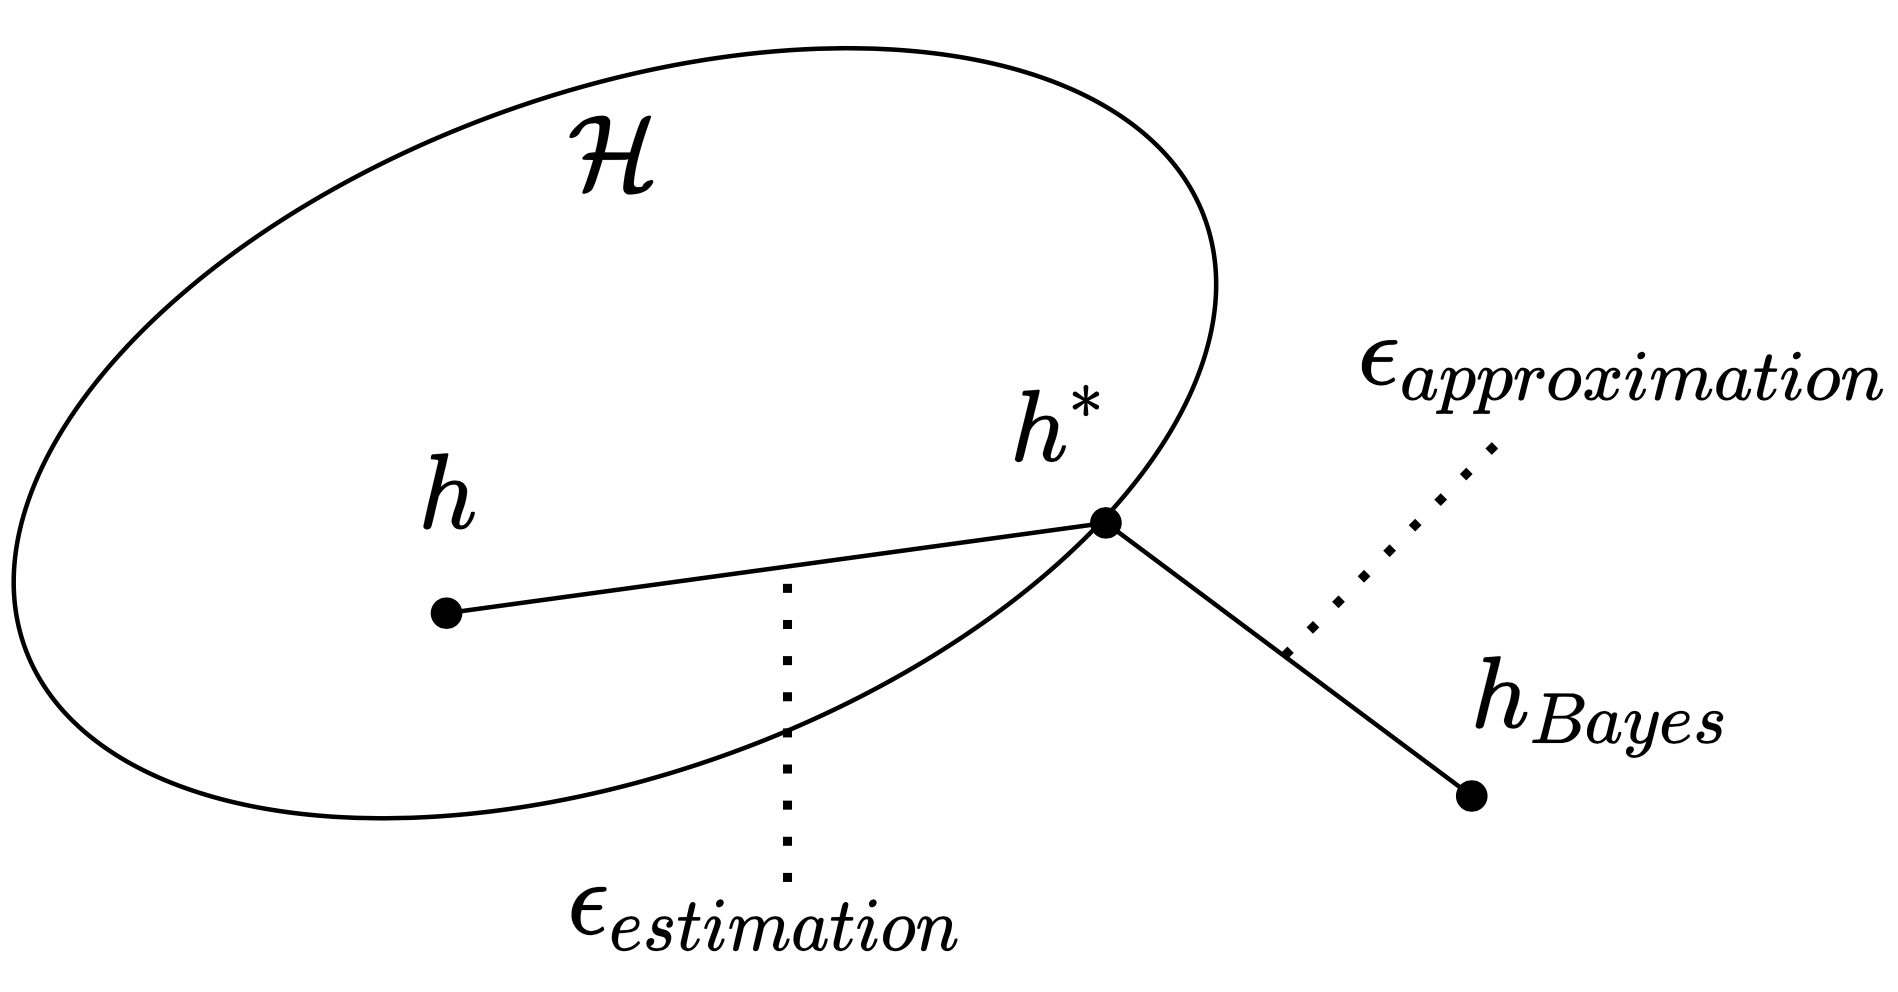
\includegraphics[width=0.6\columnwidth]{images/estimation-approximation-error.png}
    \caption{Illustration depicting the concepts}
    \label{fig:estimation-approximation-error}
\end{figure}
\begin{itemize}
  \item $h_{Bayes}$ is the Bayes classifier, with $R(h_{Bayes}) = R^*$
  \item $h^* = \inf_{h \in \mathcal{H}} R(h)$ is the hypothesis with the lowest generalization error in the hypothesis class $\mathcal{H}$
  \item $R(h)$ has both \uline{non-zero estimation error $R(h) - R(h^*)$} and \uline{approximation error $R(h^*) - R(h_{Bayes})$}
  \item \textbf{Challenge for model selection:} We \textcolor{Green}{can bound the estimation error by generalization bounds} but we \textcolor{red}{cannot do the same for the approximation error} as $R^*$ remains unknown to us.
\end{itemize}









\subsection{Strategies for Model Selection}\label{strategies-for-model-selection}




\textbf{Initially} choose a very complex hypothesis class with zero or very low empirical risk $\mathcal{H}$

\textbf{Assume} the class can be decomposed into a union of increasingly complex hypothesis classes $\mathcal{H} = \bigcup_{\gamma \in \Gamma} \mathcal{H}_\gamma$

\begin{figure}[H]
  \centering  % Remember to centre the figure
    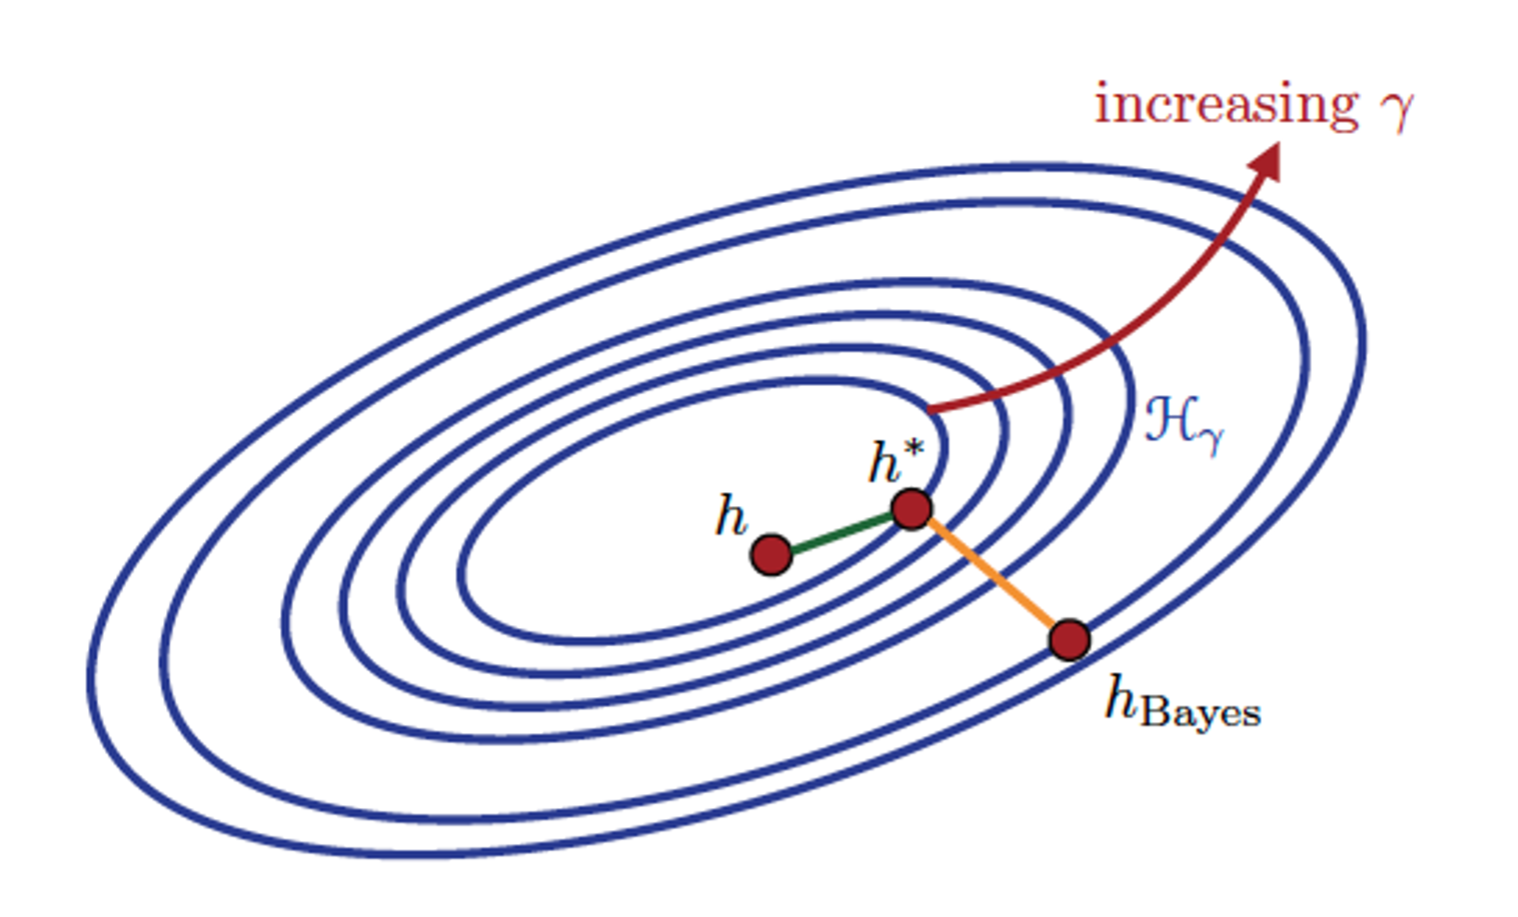
\includegraphics[width=0.8\columnwidth]{images/complex-hypothesis-classes.png}
    \caption{Illustration of hypothesis classes $\mathcal{H}$ being decomposed into a union of increasingly complex hypothesis classes}
    \label{fig:complex-hypothesis-classes}
\end{figure}

\begin{itemize}
  \item The complexity increases by parameter $\gamma$ e.g.
  \begin{itemize}
    \item $\gamma =$ degree of a polynomial function
    \item $\gamma =$ size of a neural network
    \item $\gamma =$ norm of weights of a linear regression model
  \end{itemize}
\end{itemize}

\textbf{Strategy:}
\begin{itemize}
  \item \textbf{The model selection problem then entails} \uline{choosing a parameter value $\lambda^*$ that gives the best generalization performance}
\end{itemize}

\textbf{Trade-Off:} \uline{increasing the complexity} of the hypothesis class
\begin{itemize}
  \item $(\textcolor{Green}{+})$ complexity $\rightarrow$ $(\textcolor{red}{-})$ \textcolor{Red}{approximation error} (as the class is more likely to contain a hypothesis with error close to the Bayes error)
  \item $(\textcolor{Green}{+})$ complexity $\rightarrow$ $(\textcolor{Green}{+})$ \textcolor{blue}{estimation error} (as finding the good hypothesis becomes more hard and the generalization bounds become looser (due to increasing log $\mathcal{H}_\gamma$ or the VC dimension))
\end{itemize}

\begin{figure}[H]
  \centering  % Remember to centre the figure
    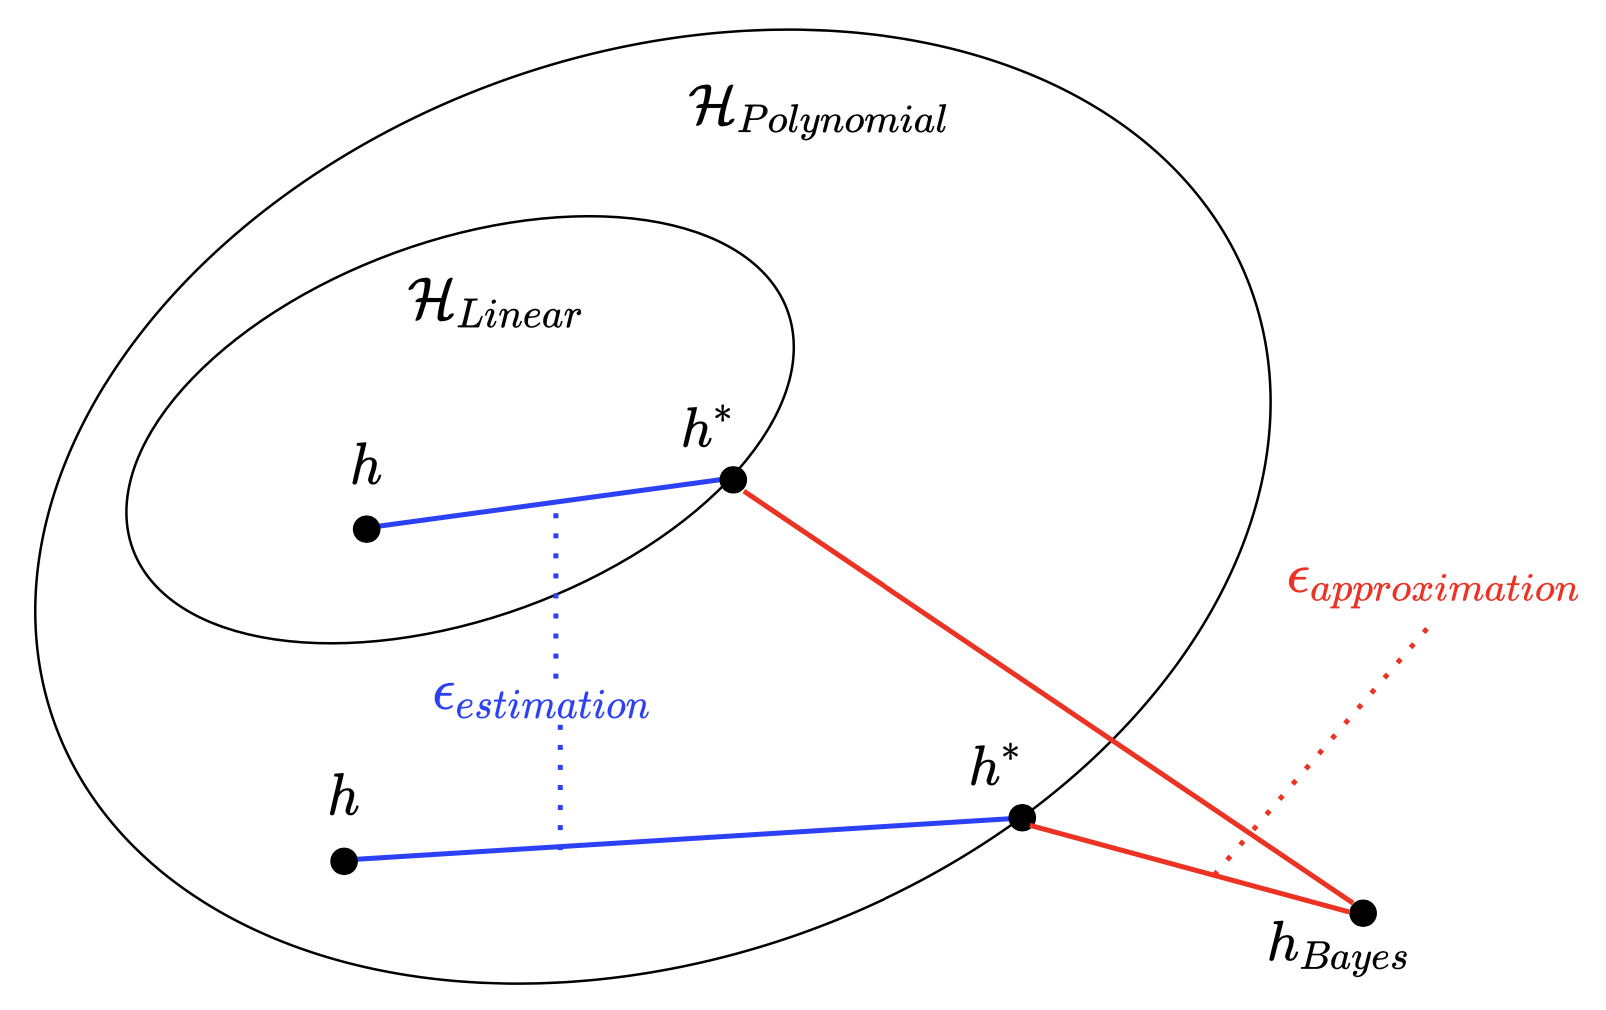
\includegraphics[width=0.9\columnwidth]{images/estimation-approximation-error-in-different-hypothesis-classes.png}
    \caption{Example case of two hypothesis $h$ from decomposed hypothesis classes $\mathcal{H}$, and their relation to $h_{Bayes}$}
    \label{fig:estimation-approximation-error-in-different-hypothesis-classes}
\end{figure}

To minimize the generalization error over all hypothesis classes, we should find a balance between the two terms













\subsubsection{Structural Risk Minimization (SRM)}\label{structural-risk-minimization}

\textbf{What:} An \textit{inductive principle} of use in ML.

\begin{itemize}
  \item \textbf{Assumes} a \textcolor{red}{\uline{countable union}} of hypothesis classes $\mathcal{H} = \bigcup_{k \geq 1} \mathcal{H}_k$, indexed by complexity parameter $k$
  \item \textbf{Model selection task:} Select the optimal index $k^*$ and the hypothesis $h \in \mathcal{H}_{k^*}$ that gives the best generalization bound
\end{itemize}


\textbf{Why:} It aims to minimize the excess risk $R(h) - R(h_{Bayes})$.

\textbf{How:} By bounding $R(h)$.
\begin{itemize}
  \item \textbf{Generalization bound for SRM (Mohri et al. 2018) in PAC-framework:} for any $\delta > 0$ with probability at least $1 - \delta$ over the draw of a sample $S$ of size $m$, we have for all $k \geq 1$ and $h \in \mathcal{H}_k$
  $$
  R(h) \leq \underbrace{\hat{R}_S(h)}_{\substack{\text{empirical error} \\ \text{on training set}}} + \underbrace{R_m(\mathcal{H}_k(h))}_{\substack{\text{Rademacher complexity of} \\ \text{least complex hypothesis class} \\ \text{(min $k$ for $\mathcal{H}$) where $h$ belongs}}} + \underbrace{\sqrt{\frac{\log{k}}{m}}}_{\substack{\text{penalty for not} \\ \text{knowing the correct $\mathcal{H}$} \\ \text{($\mathcal{H}$ selection)}}} + \sqrt{\frac{\log{\frac{2}{\delta}}}{2m}}
  $$
  \begin{itemize}
    \item See resemblance	to \ref{deneralization-bound-with-rademacher-complexity}.
  \end{itemize}
\end{itemize}


\textbf{SRM model selection algorithm:} Given a training sample $S$, picks the index $k$ and $h_S^{SRM} \in \mathcal{H}_k$ that minimizes

$$
h_S^{SRM} = \argmin_{k \geq 1, h \in \mathcal{H}_k} \hat{R}_S(h) + R_m(h_k) + \sqrt{\frac{\log{k}}{m}}
$$

\begin{figure}[H]
  \centering  % Remember to centre the figure
    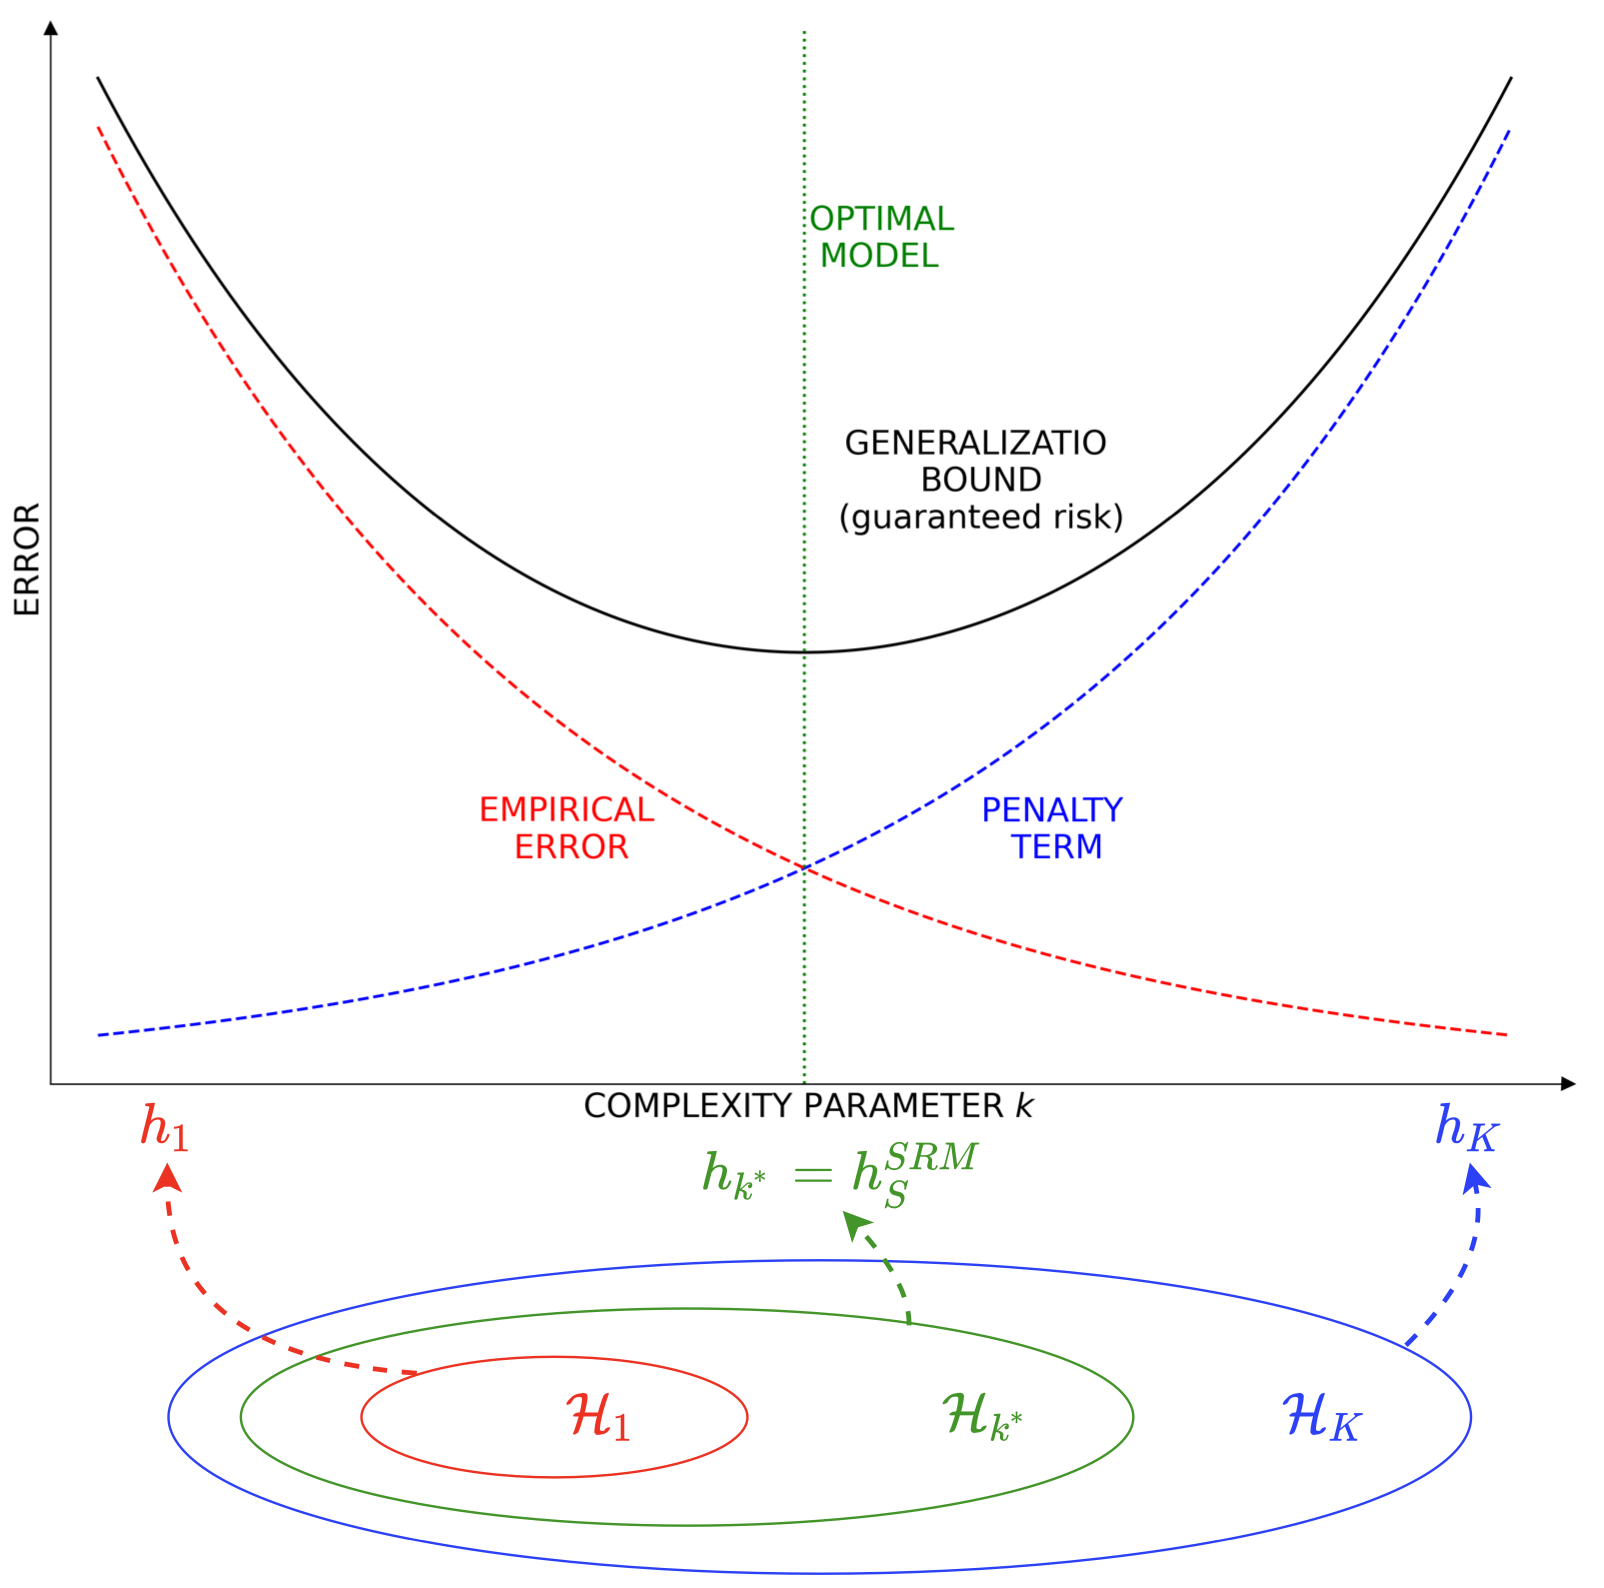
\includegraphics[width=0.8\columnwidth]{images/generalization-bound-with-rademacher-complexity.png}
    \caption{Illustration of Structural Risk Minimization (SRM) with Rademacher complexity}
    \label{fig:generalization-bound-with-rademacher-complexity}
\end{figure}


\begin{itemize}
  \item \textbf{Note} that this \textcolor{red}{may be a computationally difficult task}:
  \begin{itemize}
    \item Requires finding the hypothesis that minimizes training error for each hypothesis class separately
    \item Obtaining the empirical Rademacher complexity generally requires simulation with multiple datasets with randomized labels for each hypothesis class
  \end{itemize}
\end{itemize}


\textbf{Pros \& Cons of SRM:}

\begin{itemize}
  \item[\textcolor{Green}{$+$}] benefits from \uline{strong learning guarantees}
  \item[\textcolor{red}{$-$}] \uline{restrictive assumption} of a countable decomposition of the hypothesis class
  \item[\textcolor{red}{$-$}] \uline{large computational price}, especially when a large number of hypothesis classes $\mathcal{H}_k$ has to be processed
\end{itemize}












\subsubsection{Regularization-based algorithms}\label{regularization-based-algorithms}

\textbf{What:} An alternative model selection approach to SRM.

\begin{itemize}
  \item \textbf{Assumes} a very complex family $\mathcal{H} = \bigcup_{\gamma \geq 0} \mathcal{H}_\gamma$ of \textcolor{Green}{\uline{uncountable union}} of nested hypothesis classes $\mathcal{H}_\gamma$
\end{itemize}

\textbf{How:}

This extension to the SRM method would then ask to minimize:
$$
= \argmin_{\gamma \geq 0, h \in \mathcal{H}_\gamma} \hat{R}_S(h) + R_m(h_\gamma) + \sqrt{\frac{\log{\gamma}}{m}}
$$
\begin{itemize}
  \item This problem seems to require evaluating the Rademacher complexity of an uncountably infinite number of hypothesis classes $\mathcal{H}_\gamma$ $\rightarrow$ \textcolor{red}{Need efficient algorithms to do this}
\end{itemize}

However this kind of model selection is \textcolor{Green}{efficient for} the class of \textbf{linear functions $x \rightarrow w^T x$}

\begin{itemize}
  \item The classes as parametrized by the norm $||w||$ of the weight vector bounded by $\gamma$:
  $$
  \mathcal{H}_\gamma = \{x \rightarrow w^T x : ||w|| \leq \gamma\}
  $$
  \begin{itemize}
    \item The norm $||w||$ is typically eiteher:
    \begin{itemize}
      \item \textbf{$L^2$ norm (Also called Euclidean norm or 2-norm):}
      \begin{itemize}
        \item used e.g. in support vector machines and ridge regression
      $$
      ||w||_2 = \sqrt{\sum_{j=1}^n w_j^2}
      $$
      \end{itemize}
      \item \textbf{$L^1$ norm (Also called Manhattan norm or 1-norm):}
      \begin{itemize}
        \item used e.g. in LASSO regression
      $$
      ||w||_1 = \sum_{j=1}^n |w_j|
      $$
      \end{itemize}
    \end{itemize}
  \end{itemize}
\end{itemize}


\textbf{Computational shortcut: for $L^2$-norm:} the \textcolor{blue}{empirical Rademacher complexity} of this class can be bounded analytically!
\begin{itemize}
  \item Let $S \subset \{x \; | \;\; ||x|| \leq r \}$ be a sample of size m and let $\mathcal{H}_\gamma = \{x \rightarrow w^T x : ||w||_2 \leq \gamma\}$. Then
  $$
  \hat{R}_S(\mathcal{H}_\gamma) \leq \sqrt{\frac{r^2 \gamma^2}{m}} = \frac{r \gamma}{\sqrt{m}}
  $$
  \begin{gather*}
    \textbf{Where:} \\
    \textbf{r}: \text{upped bound for length of the input vector $||x||$} \\
    \textbf{$\gamma$}: \text{upped bound for length of the weight vector $||w||_2$}
  \end{gather*}
  \begin{itemize}
    \item Thus the \textbf{Rademacher complexity} \textcolor{Green}{depends linearly on the upper bound $\gamma$ norm of the weight vector}, as $r$ and $m$ are constant for any fixed training set
    \item So we can use $||w||$ as a efficiently computable upper bound of $hat{R}_S(\mathcal{H}_\gamma)$
  \end{itemize}
\end{itemize}


\textbf{Regularized learning problem:} minimize
$$
\argmin_{h \in \mathcal{H}} \hat{R}_S(h) + \lambda \Omega(h)
$$
\begin{gather*}
  \textbf{Where:} \\
  \textbf{$\hat{R}_S(h)$}: \text{empirical error} \\
  \textbf{$\Omega(h)$}: \text{regularization term which increases when the} \\ \text{complexity of the hypothesis class increases} \\
  \textbf{$\lambda$}: \text{regularization parameter, which is usually set by cross-validation}
\end{gather*}









\subsubsection{Model selection using a validation set}\label{validation-set}

\textbf{What:} Using the given dataset for \uline{\textit{empirical model selection}}.

\textbf{When:} \textit{If} the algorihm has input parameters (\uline{hyperparameters}) that define/affect the model complexity.

\textbf{How:}
\begin{enumerate}
  \item \textbf{Split} the data into \uline{training}, \uline{validation} and \uline{test} sets
  \begin{figure}[H]
    \centering  % Remember to centre the figure
      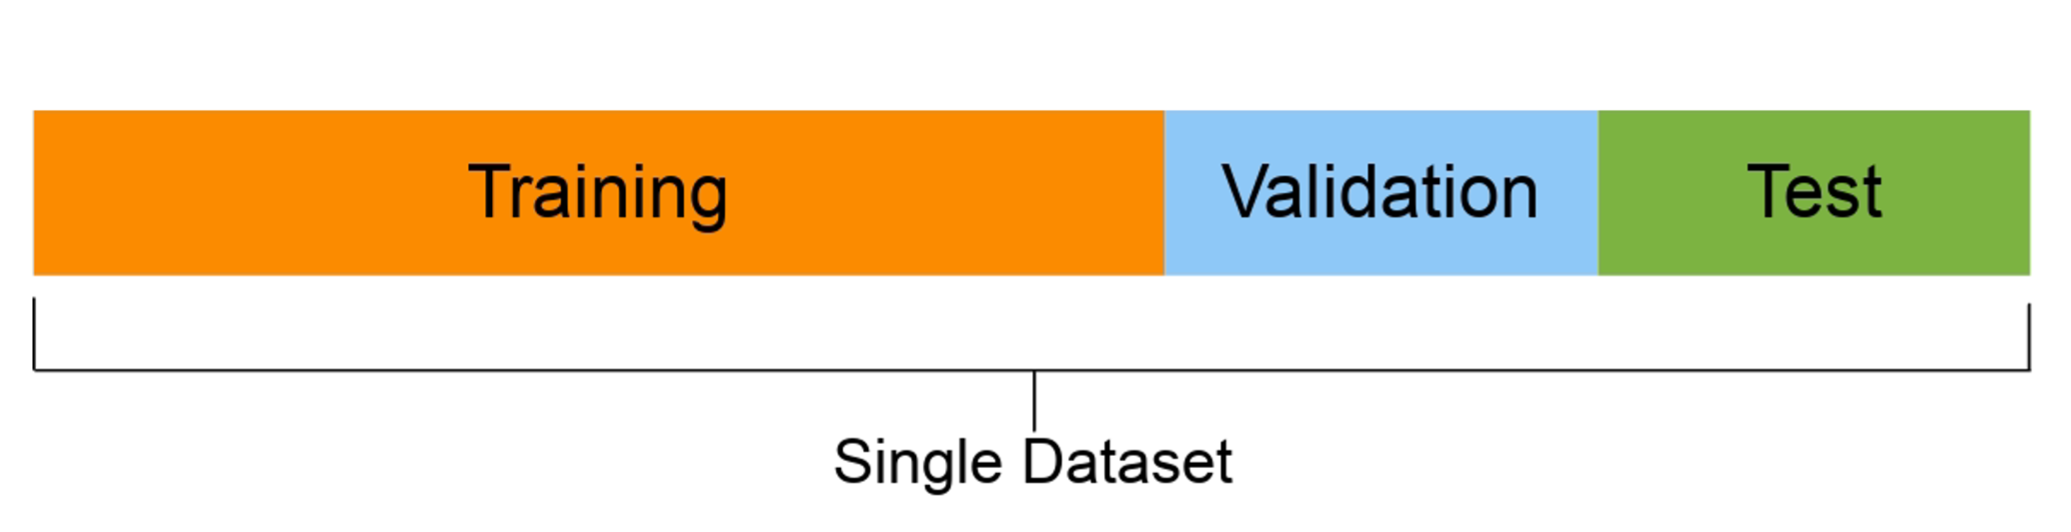
\includegraphics[width=0.6\columnwidth]{images/data-split.png}
      \label{fig:data-split}
  \end{figure}
  \item Use \textbf{\textcolor{blue}{grid search}} to \uline{find the hyperparameters combination that gives the best performance on the validation set}
  \begin{itemize}
    \item In its \textbf{basic form} it \uline{goes through all combinations of parameter values, given a set of candidate values} for each parameter
    \begin{itemize}
      \item \textbf{With many hyperparameters} the search becomes \textcolor{red}{computationally hard} due to exponentially exploding search space
    \end{itemize}
  \end{itemize}
  \item \textbf{Retrain a final model} using the \textit{optimal parameter combination}, use both the \uline{training and validation data} for training
  \item \textbf{Evaluate the performance} of the final model on the \uline{test set}
\end{enumerate}


\textbf{Sets:}
\begin{itemize}
  \item \textbf{Training set:} used to \uline{fit (optimize) the parameters (weights)} of the model.
  \item \textbf{Validation set:} used to \uline{avoid overfitting}. It provides an unbiased evaluation of a model fit on the training data set while tuning the model's hyperparameters.
  \item \textbf{Test set:} used to obtain \uline{reliable performance estimate}.
\end{itemize}

\bigskip

\textbf{Deciding on set sizes:}
\begin{itemize}
  \item The \textbf{larger the training set}, the \textcolor{Green}{better the generalization error} will be (e.g. by PAC theory)
  \item The \textbf{larger the validation set}, the \textcolor{Green}{less variance there is in the test error estimate}.
  \item When the \textbf{dataset is small} generally the \uline{\textbf{training set} is taken to be as large as possible}, typically 90\% or more of the total
  \item When the \textbf{dataset is large}, \uline{\textbf{training set} size is often taken as big as the computational resources allow}
\end{itemize}

\bigskip

\textbf{Stratification:} is a process that tries to \uline{ensure similar class distributions across the different sets}.
\begin{itemize}
  \item \textbf{Motivation:} Class distributions of the training and validation sets should be as similar to each another as possible, \textcolor{red}{otherwise there will be extra unwanted variance}
  \item \textbf{Simple approach:} \uline{divide all classes separately into the training and validation sets} and the merge the class-specific training sets into global training set and class-specific validation sets into a global validation set.
  \begin{figure}[H]
    \centering  % Remember to centre the figure
      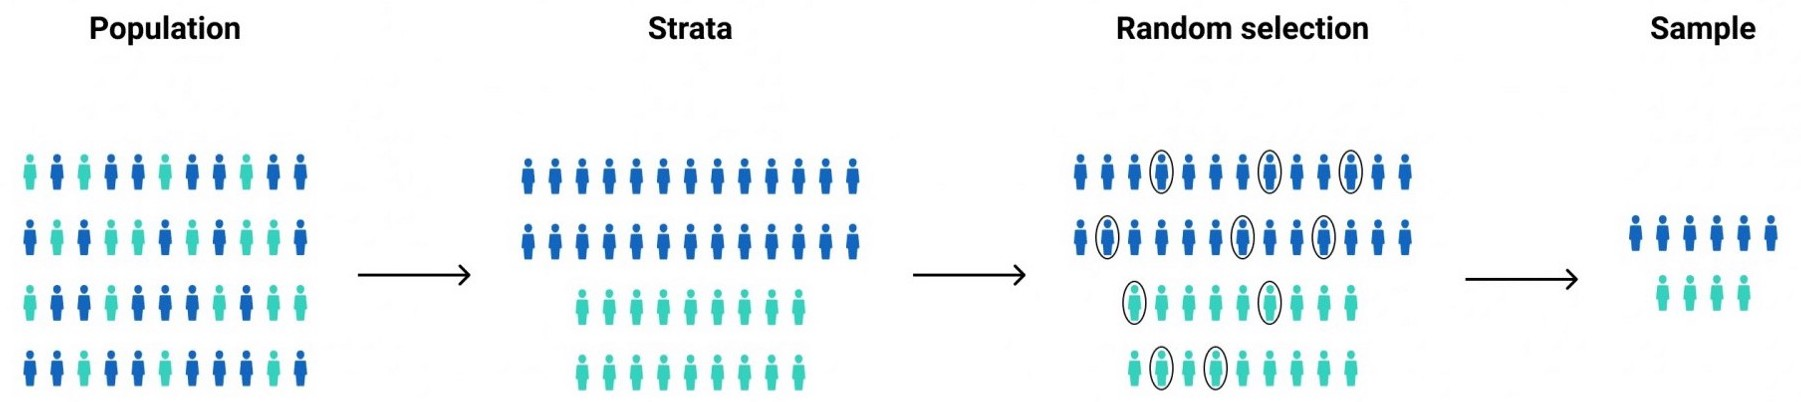
\includegraphics[width=1.0\columnwidth]{images/stratified-sampling.jpg}
      \caption{Illustration of stratified sampling}
      \label{fig:stratified-sampling}
  \end{figure}
\end{itemize}









\subsubsection{Cross-validation}\label{cross-validation}

\textbf{Why:} \textcolor{red}{One split} of data into training, validation and test sets \textcolor{red}{may not be enough, due to randomness}:

\begin{itemize}
  \item The training and validation sets might be small and contain \uline{noise or outliers}
  \item There might be some \uline{randomness in the training procedure} (e.g. initialization)
\end{itemize}


\textbf{How:} Fighting the randomnes by \uline{averaging the evaluation measure over multiple (training, validation) splits}
\begin{itemize}
  \item $\rightarrow$ The \textbf{best hyperparameter values} are chosen as those that have the \uline{best average performance over the $n$ validation sets}.
\end{itemize}

\bigskip


Various cross-validation schemes can be used to tackle the variance of the performance estimates.


\textbf{$n$-Fold Cross-Validation}

\begin{enumerate}
  \item First \textbf{set a side} a separate \uline{test set}
  \item Then \textbf{split the remaining data randomly} into \uline{$n$ equal-sized parts (or folds)}
  \begin{itemize}
    \item $n = 5$ or $n = 10$ are typical numbers used in practice
  \end{itemize}
  \item Keep \textbf{one of the $n$ folds} as the \uline{validation set} (light blue in the Figure) and combine the \textbf{remaining $n - 1$ folds} to form the \uline{training set} for the split
  \begin{figure}[H]
    \centering  % Remember to centre the figure
      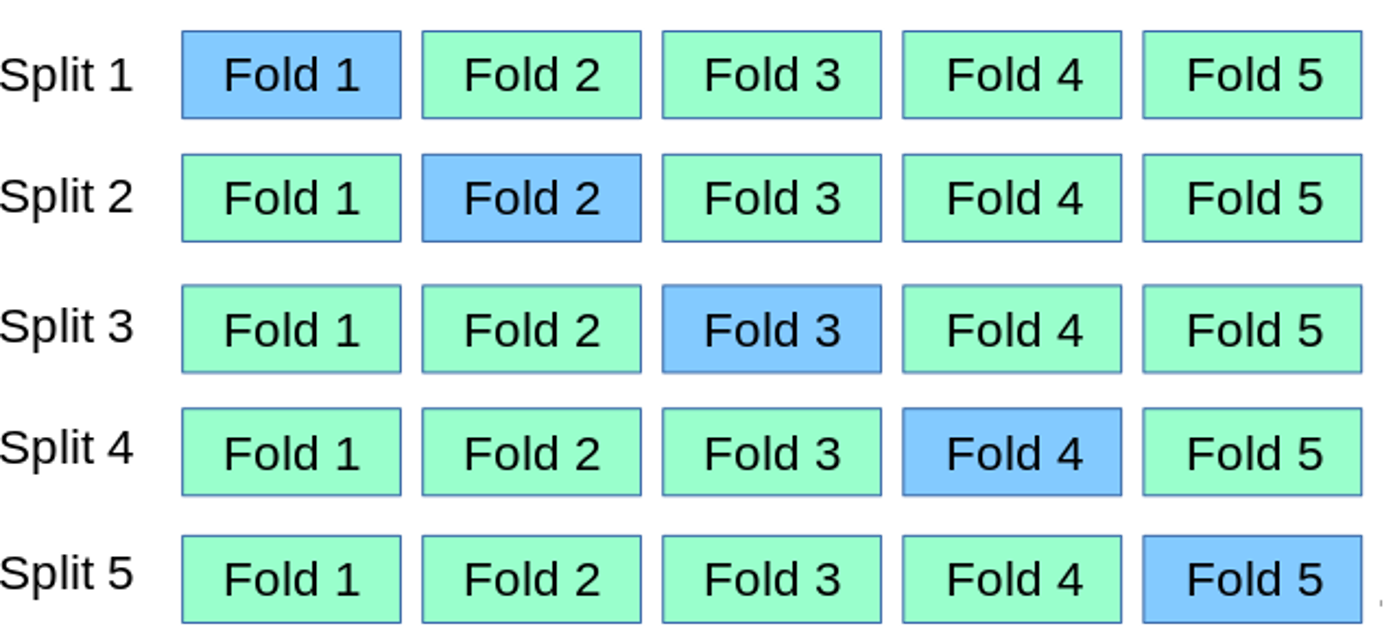
\includegraphics[width=0.6\columnwidth]{images/n-fold-cv.png}
      \label{fig:n-fold-cv}
  \end{figure}
\end{enumerate}



\bigskip


\textbf{Leave-one-out Cross-Validation (LOO)}
\begin{itemize}
  \item \textbf{How:} given a dataset of $m$ examples, only one example is left out as the validation set and training uses the $m - 1$ examples.
  \item \textbf{Has good theoretical properties:} This gives an \uline{unbiased estimate of the average generalization error over samples of size $m - 1$} (Mohri, et al. 2018, Theorem 5.4.)
  \item However, \textbf{if $m$ is large}, it is \textcolor{red}{comptationally demanding} to compute
\end{itemize}


\bigskip


\textbf{Nested cross-validation}
\begin{itemize}
  \item \textbf{Motivation:} only using a \textbf{single test set} \textcolor{red}{may result in unwanted variation} $\rightarrow$ Nested cross-validation \textcolor{Green}{solves this problem} by using \uline{two cross-validation loops}
  \item \textbf{Process:}
  \begin{enumerate}
    \item The dataset is initially divided into $n$ outer folds
    \item \textbf{Outer loop} uses \uline{\textbf{1 fold} at a time as a \textbf{test set}},
    \item The \uline{\textbf{remaining folds} of the data is used in the \textbf{inner fold}}
    \begin{itemize}
      \item \textbf{Inner loop} \uline{splits} the remaining exampls into $k$ folds, \uline{1 fold for validation}, and \uline{$k - 1$ for training}
    \end{itemize}
    \item The \uline{average performance over the $n$ test sets} is computed as the \textbf{final performance estimate}
  \end{enumerate}
  \begin{figure}[H]
    \centering  % Remember to centre the figure
      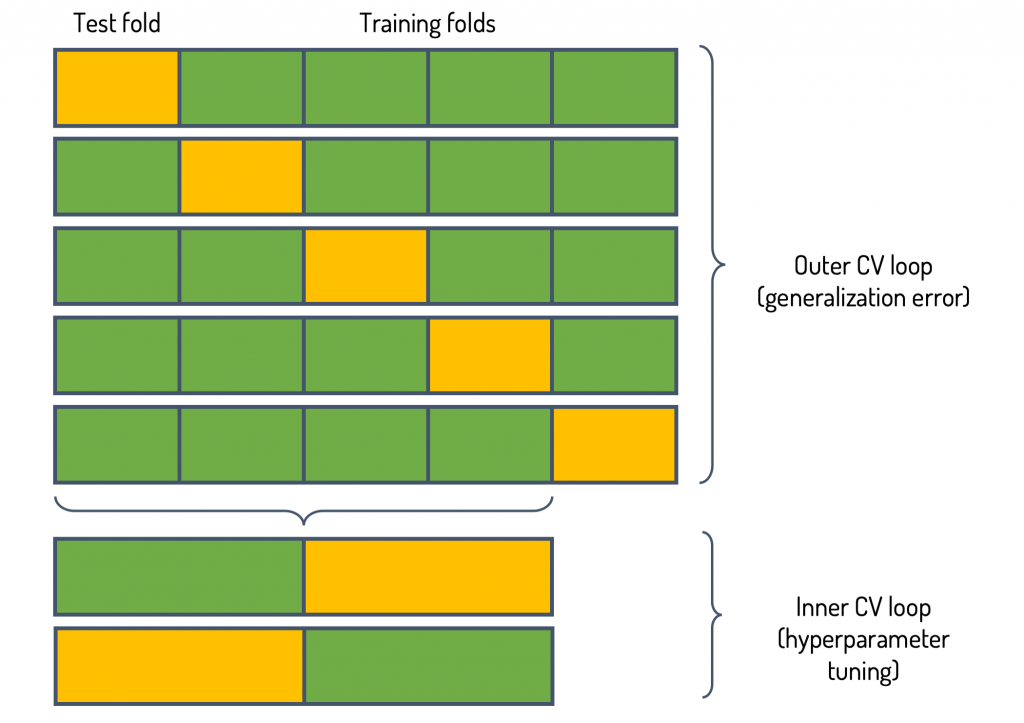
\includegraphics[width=0.8\columnwidth]{images/nested-cv.png}
      \caption{Illustration of $5 \times 2$ nested cross-validation}
      \label{fig:nested-cv}
  \end{figure}
\end{itemize}


\begin{center}\rule{3in}{0.4pt}\end{center}
















\newpage
\part{Algorithms and Models}
\newpage











\section{Loss functions}\label{loss-functions}


At its core, a loss function is a measure of how good your prediction model does in terms of being able to predict the expected outcome (or value).

Loss functions measure how far an estimated value is from its true value. A loss function maps decisions to their associated costs. Loss functions are not fixed, they change depending on the task in hand and the goal to be met.

Convexity is more crucial than the differentiability.
Differentiability is also very usefull.







\subsection{Minimizing loss functions}\label{minimizing-loss-functions}

\subsubsection{Gradient of a Function (Calculus Refresh)}

\textcolor{blue}{\textbf{Derivative}} is a way to show \textbf{instantaneous rate of change (slope of the tangent line at a point on a graph):} that is, the \uline{amount by which a function is changing at one given point}.
\begin{itemize}
  \item Common notations:
  \begin{align*}
    \frac{d y}{d x} & \text{, meaning the difference in $y$ divided by the difference in $x$} \\
    f'(x) & \text{, meaning the derivative of function $f$ at point $x$}
  \end{align*}
  \item Important in optimization because the \textbf{zero derivatives} might indicate a \uline{minimum}, \uline{maximum}, or \uline{saddle point}.
\end{itemize}

\textcolor{blue}{\textbf{Gradient}} \textcolor{blue}{of} a \uline{scalar-valued differentiable function $f$ of several variables} \textcolor{blue}{is} the \uline{vector field (or vector-valued function) $\nabla f$} \textcolor{blue}{whose} \uline{value at a point $p$ is the vector whose components are the partial derivatives of $f$ at $p$}. More generally, it is a \textbf{vector that points in the direction in which the function grows the fastest}. value at a point

\begin{itemize}
  \item Common notations:
  \begin{align*}
    \nabla f & \text{, meaning the gradient of a function $f$} \\
    -\nabla f & \text{, meaning the negative gradient of a function $f$}
  \end{align*}
\end{itemize}

When working with gradient descent, you’re interested in the direction of the fastest decrease in the cost function. This direction is determined by the negative gradient, $-\nabla f$.



\subsection{Loss functions for classification}\label{loss-functions-for-classification}

See more \href{https://en.wikipedia.org/wiki/Loss_functions_for_classification}{here}.

\textbf{Zero-One loss}
\begin{itemize}
  \item It assigns 0 to loss for a correct classification and 1 for an incorrect classification.
  \item \textbf{Specs:}
  \begin{itemize}
    \item The main source of difficulty is the ”step function” shape of the zero-one loss function
    \begin{itemize}
      \item It is \textcolor{red}{non-differentiable} $\rightarrow$ \textcolor{red}{cannot optimize using gradient approaches}
      \item It is \textcolor{red}{non-convex} $\rightarrow$ optimizer \textcolor{red}{susceptible to fall in local minima}
    \end{itemize}
  \end{itemize}
\end{itemize}

A convex loss function makes it easier to find a global optimum and to know when one is reached. There are multiple surrogate losses that are convex and differentiable upper bounds to zero-one loss.


\textbf{Hinge loss} - used in Support vector machines

\begin{itemize}
  \item \textbf{Specs:}
  \begin{itemize}
    \item It is \textcolor{red}{non-differentiable}, but has a subgradient with respect to model parameters w
  \end{itemize}
\end{itemize}


\textbf{Exponential loss} - used in Boosting


\textbf{Logistic loss} - used in Logistic regression



\begin{center}\rule{3in}{0.4pt}\end{center}




















\section{Linear classification}\label{linear-classification}

\textbf{What:} Performing \uline{classification based on the value of a linear combination of weights and features}.

\textbf{Hypothesis class:}
$$
\mathcal{H} = \{x \rightarrow \text{sgn}\left(\sum_{j=1}^d w_j x_j + w_0\right) \;\;|\;\; w \in \mathbb{R}^d, w_0 \in \mathbb{R}\}
$$

\begin{itemize}
  \item Consists of \textbf{linear classifiers} that \uline{map each example in one of the classes}:
  $$
  h(x) = \text{sgn}\left(\sum_{j=1}^d w_j x_j + w_0\right) = w^T x + w_0
  $$
  \begin{itemize}
    \item \uline{$\text{sgn}(a)$ is the \textit{sign function}}. E.g. for binary classification:
    $$
    \text{sgn}(a) =
    \begin{cases}
      +1 & a \geq 0 \\
      -1 & a < 0
    \end{cases}
    $$
  \end{itemize}
\end{itemize}


\textbf{Attractive properties:}
\begin{itemize}
  \item They are \textcolor{Green}{fast to evaluate} and \textcolor{Green}{takes small space to store} ($O(d)$ time and space)
  \item \textcolor{Green}{Easy to understand}: $|w_j|$ shows the importance of variable $x_j$ and its sign tells if the effect is positive or negative
  \item Linear models have relatively \textcolor{Green}{low complexity} (e.g. $VCdim = d + 1$) so they can be \textcolor{Green}{\uline{reliably estimated from limited data}}
  \item \textcolor{Orange}{Good practise is to try a linear model before something more complicated}
\end{itemize}












\subsection{Learning linear classifiers}\label{learning-with-linear-classificiers}


\begin{tcolorbox}[colback=yellow!5,colframe=yellow!75!black,title={Change of representation}]
For presentation is is convenient to subsume term $w_0$ into the weight vector and augment all inputs with a constant 1:
$$
w \Leftarrow
\begin{bmatrix}
w \\
w_0
\end{bmatrix} \;\;\;\;
x \Leftarrow
\begin{bmatrix}
x \\
1
\end{bmatrix}
$$

The models have the same value for the discriminant:
$$
\begin{bmatrix}
w \\
w_0
\end{bmatrix}^T
\begin{bmatrix}
x \\
1
\end{bmatrix}
= w^T x + w_0
$$
\end{tcolorbox}


\textbf{Checking for prediction errors:}

\begin{itemize}
  \item When the labels are $Y = \{-1, +1\}$ for a training example $(x, y)$ we have for $g(x) = w^T x$
  $$
  \text{sgn}(g(x)) =
  \begin{cases}
    y & \text{if $x$ is correctly classified} \\
    -y & \text{if $x$ is incorrectly classified} \\
  \end{cases}
  $$
  \item Alternative we can just \uline{multiply with the correct label} to \textbf{check for misclassification:}
  $$
  yg(x) =
  \begin{cases}
    \geq 0 & \text{if $x$ is correctly classified} \\
    < 0 & \text{if $x$ is incorrectly classified} \\
  \end{cases}
  $$
\end{itemize}

\textbf{Margin:} the \uline{minimal distance of any training point to the hyperplane} (decision boundary).
\begin{itemize}
  \item \textbf{Geometric margin} for an example $x$ is given by $\gamma(x) = yg(x) / ||w||$
  \item \textbf{Functional margin} (unnormalized version) for an example $x$ is given by $\gamma(x) = yg(x)$
  \begin{figure}[H]
    \centering  % Remember to centre the figure
      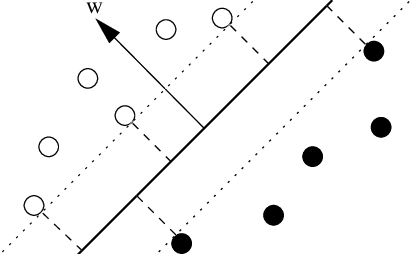
\includegraphics[width=0.6\columnwidth]{images/margin.png}
      \caption{Example where margin is the distance between the dotted lines and the thick line}
      \label{fig:margin}
  \end{figure}
\end{itemize}








\subsection{Perceptron}\label{perceptron}

\textbf{What:} is a simple algorithm to train linear classifiers on linearly separable data.

\textbf{How:} learns a hyperplane separating two classes:
$$
g(x) = w^T x
$$

\begin{itemize}
  \item It processes incrementally a set of training examples
  \begin{itemize}
    \item \textbf{At each step}, it finds a training example $x_i$ that is incorrectly classified by the current model
    \item It \textbf{updates the model} by adding the example to the current weight vector together with the label: $w^{(t+1)} \leftarrow w^{(t)} + y_i x_i$
    \item This process is \textbf{continued until} incorrectly predicted training examples are not found
  \end{itemize}
\end{itemize}


\textbf{Convergence:}
\begin{itemize}
  \item \textcolor{red}{Only if} the two classes are \textbf{linearly separable}
  \item \textcolor{red}{Doesn't stop if} \textbf{non-separable training set}
  \item \textbf{Theorem (Novikoff):}
  \begin{itemize}
    \item Will stop after at most $t \leq (\frac{2R}{\gamma})^2$ iterations
    \begin{itemize}
      \item $\gamma$: The \uline{largest achievable geometric margin so that all training examples have at least that margin}
      \item R: The \uline{smallest radius of the d-dimensional ball that encloses the training data}
    \end{itemize}
    \begin{figure}[H]
      \centering  % Remember to centre the figure
        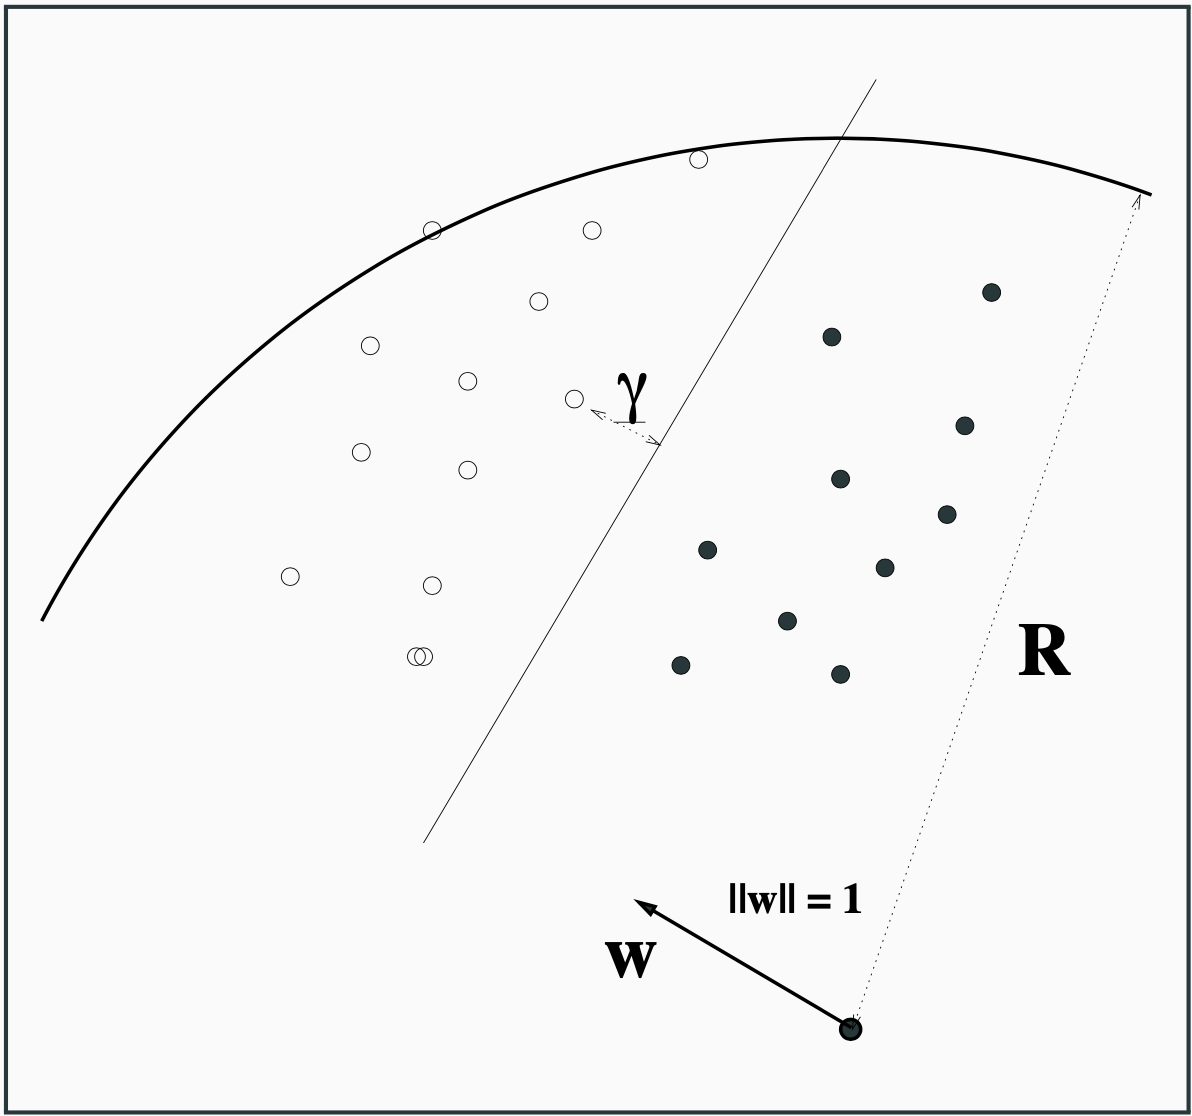
\includegraphics[width=0.6\columnwidth]{images/perceptron-convergence.png}
        \label{fig:perceptron-convergence}
    \end{figure}
  \end{itemize}
\end{itemize}







\subsection{Logistic Regression}\label{logistic-regression}

\textbf{What:} is a classification method that can be interpreted as maximizing odds ratios of conditional class probabilities.

\begin{itemize}
  \item It gets its name from the \textbf{logistic function} that \uline{maps a real valued input $z$ onto the interval $0 < \phi_{logistic}(z) < 1$}
  $$
  \phi_{logistic}(z) = \frac{1}{1 + \exp(-z)} = \frac{\exp(z)}{1+\exp(z)}
  $$
  \begin{figure}[H]
    \centering  % Remember to centre the figure
      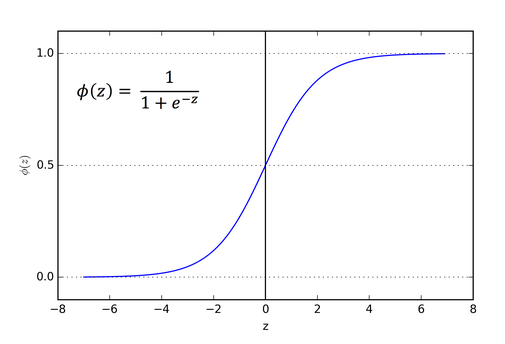
\includegraphics[width=0.7\columnwidth]{images/logistic-function.png}
      \label{fig:logistic-function}
  \end{figure}
\end{itemize}



\begin{center}\rule{3in}{0.4pt}\end{center}




















\section{Support Vector Machines (SVMs)}\label{support-vector-machines}

\textbf{What:} classification methods based on the principle of \uline{margin maximization}. Commonly Performing \uline{nonlinear classification with kernel methods}.

\textbf{How:} SVMs can be efficiently optimized using Stochastic gradient techniques specially developed for piecewise differentiable functions, such as the Hinge loss.

\textbf{Main idea:}

\begin{enumerate}
  \item Start with \textbf{data} in a relatively \uline{low dimension}
  \item Move the \textbf{data} into a \uline{higher dimension} (using Kernel methods)
  \item Find a Support Vector Classifier that \uline{separates the higher dimensional data} into groups
\end{enumerate}






\subsection{Maximum margin hyperplane}\label{maximum-margin-hyperplane}

\textbf{What:} Hyperplane $\mathbf{w}^T x = 0$ that lies furthest away from the training data (maximizing the minimum margin of the training examples):

\begin{gather*}
\text{Maximize } \gamma \\
\text{w.r.t. variables } \mathbf{w} \in \mathbb{R}^d \\
\text{Subject to } \frac{y_i \mathbf{w}^T \mathbf{x}_i}{||\mathbf{w}||} \geq \gamma \text{, for all } i = 1, ..., m
\end{gather*}

\bigskip

\textbf{Why:} Support vector machines (SVM) are based on this principle.

\textbf{Good properties:}

\begin{itemize}
  \item Robustness: small change in the training data will not change the classifications too much
  \item Theoretically a large margin is tied to a low generalization error
  \item It can be found efficiently through incremental optimization
\end{itemize}

\bigskip

\textbf{Process:} How to maximize the margin:

\begin{itemize}
  \item Optimizing $\gamma$ does not give us a unique optimal weight vector $\mathbf{w}^*$
  \item To get an unique answer, let us multiply the constraint on the geometric margin by $||\mathbf{w}||$ to obtain a an equivalent constraint on the functional margin
  \begin{gather*}
  \frac{y_i \mathbf{w}^T \mathbf{x}_i}{||\mathbf{w}||} \geq \gamma \\
  y_i \mathbf{w}^T \mathbf{x}_i \geq \gamma ||\mathbf{w}|| \\
  \end{gather*}
  \begin{itemize}
    \item Now fix the functional margin to 1: $\gamma ||\mathbf{w}|| = 1$ which gives $\gamma = \frac{1}{||\mathbf{w}||}$
    \item To maximize $\gamma$, we should minimize $||\mathbf{w}||$ with the constraint of having functional margin of at least 1
  \end{itemize}
\end{itemize}


\bigskip


\textbf{Hard margin Support Vector Machine (SVM)} solves the margin maximization as follows:

\begin{gather*}
\text{Minimize } \frac{1}{2} ||\mathbf{w}||^2 \\
\text{w.r.t. variables } \mathbf{w} \in \mathbb{R}^d \\
\text{Subject to } y_i \mathbf{w}^T \mathbf{x}_i \geq 1 \text{, for all } i = 1, ..., m
\end{gather*}

\begin{itemize}
  \item We are minimizing the half of the squared norm of the weight vector, which gives the same answer as minimizing the norm, but easier to optimize
  \item This is \textbf{equivalent of} \uline{finding the maximal geometric margin} over the same data
\end{itemize}

The so called hard margin support-vector machine \textcolor{red}{assumes linearly separable data}







\subsection{Soft-Margin SVM}\label{soft-margin-svm}

\textbf{What:} relaxed margin constraints

\textbf{Why:} allows non-separable data

\textbf{How:} To allow non-separable data, we allow the functional margin $y_i \mathbf{w}^T \mathbf{x}_i$ of some data points $\mathbf{x}_i$ to be smaller than 1 by a slack variable $\xi \geq 0$.

\begin{itemize}
  \item Relaxed margin constraint:
  $$
  y_i \mathbf{w}^T \mathbf{x}_i \geq 1 -\xi \;,\;\; (\xi \geq 0)
  $$
\end{itemize}

\begin{figure}[H]
\centering
  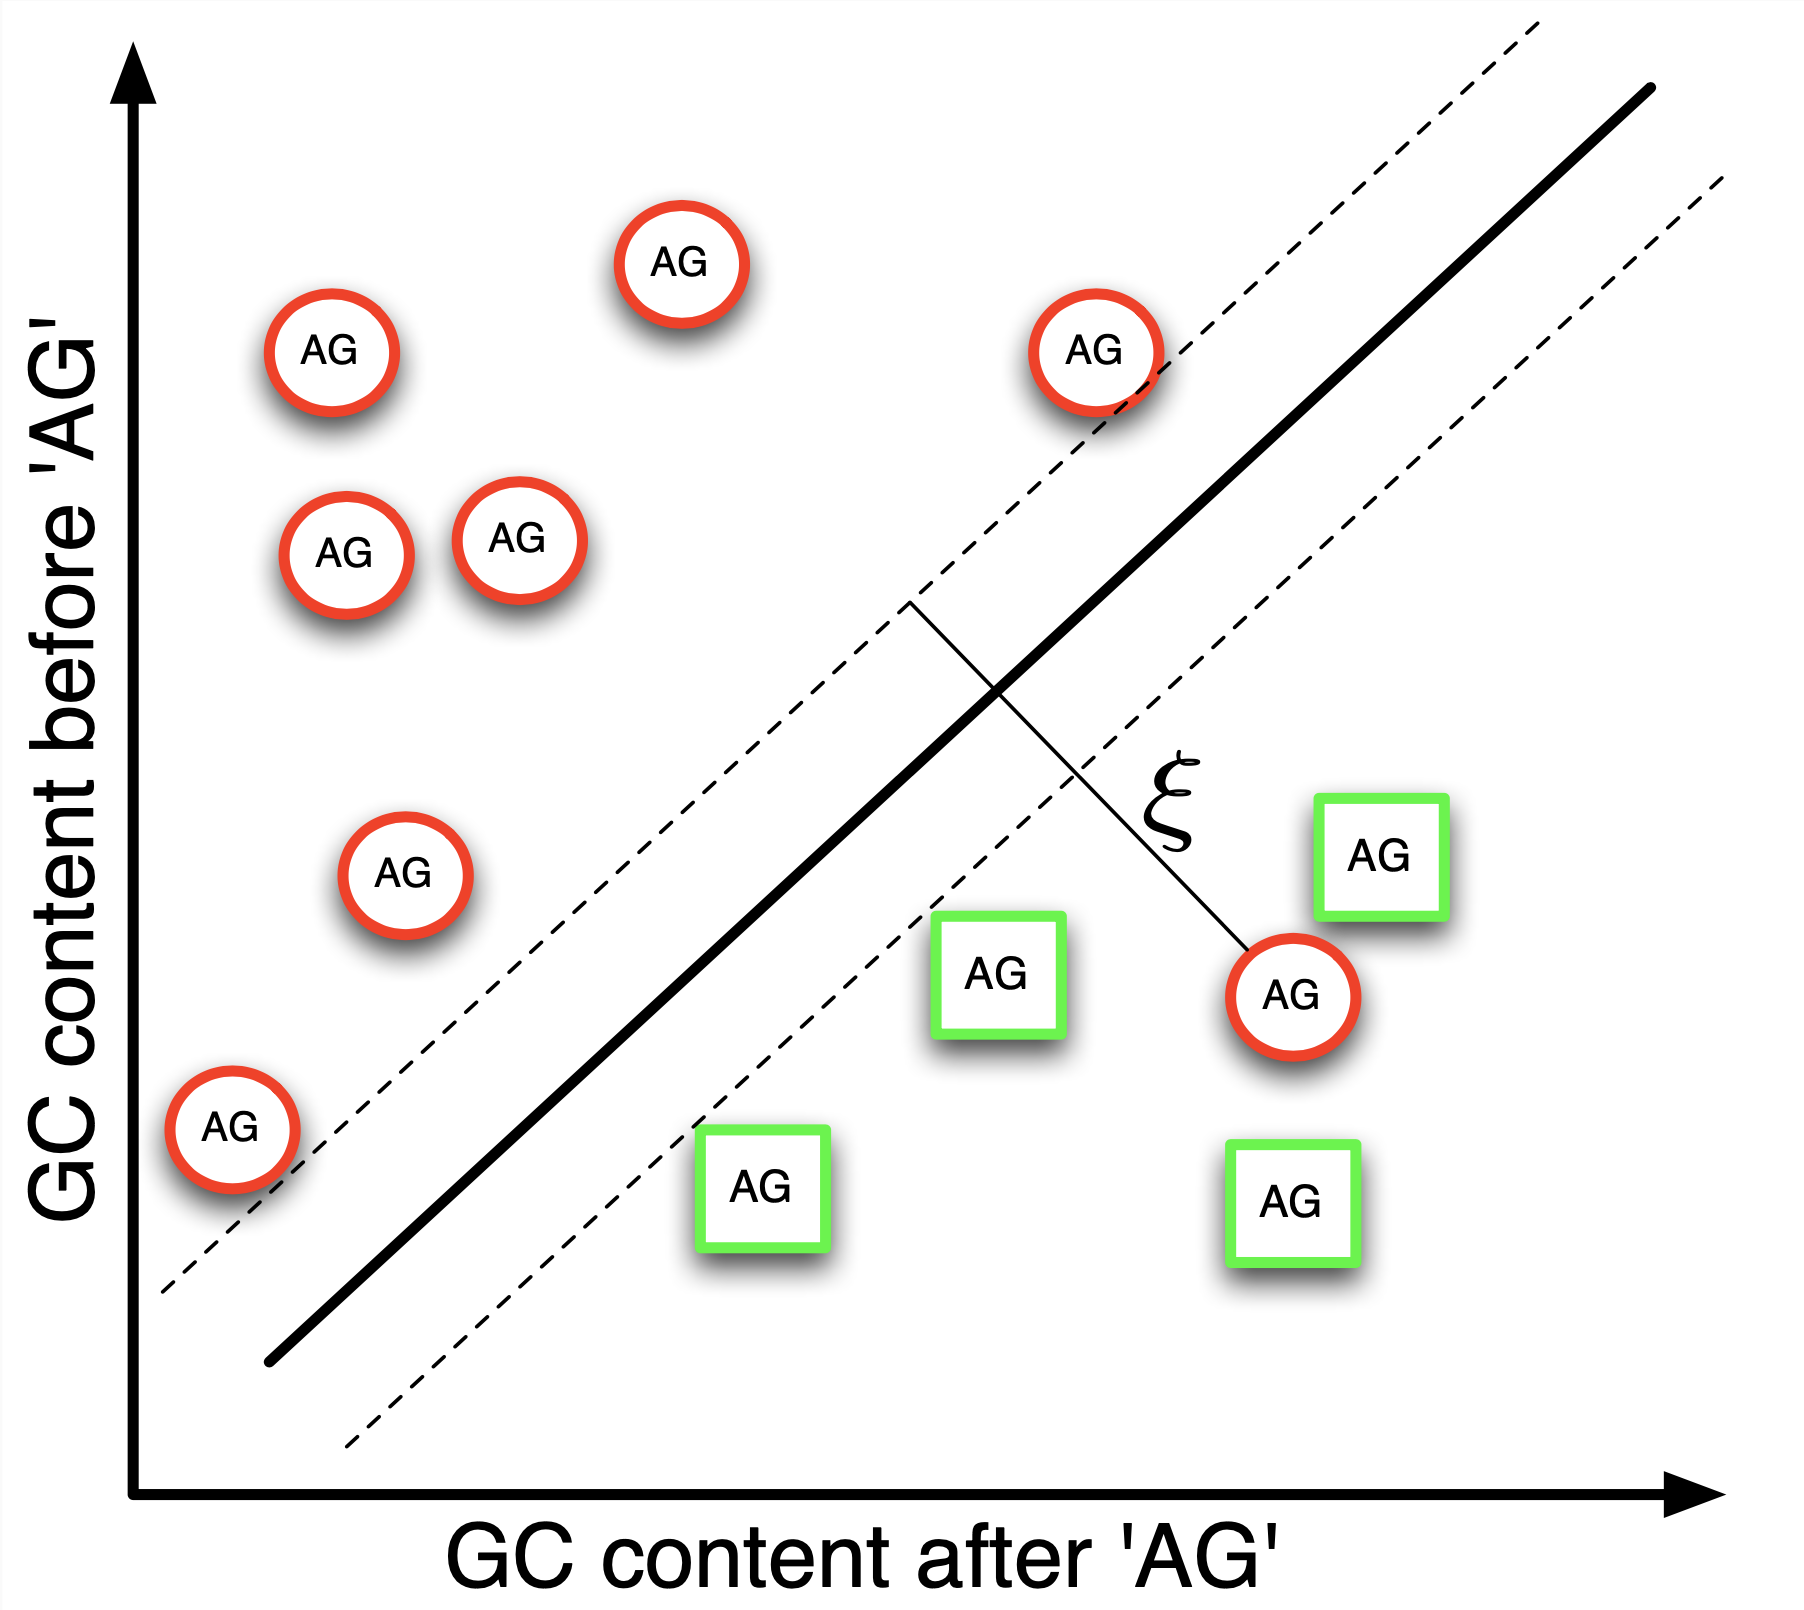
\includegraphics[width=0.6\columnwidth]{images/slack-variables-for-soft-margin-classifiers.png}
  \caption{Examples of slack variables for soft margin classifiers.}
  \label{fig:slack-variables-for-soft-margin-classifiers}
\end{figure}
\begin{itemize}
  \item $\xi_i = 0$ corresponds to having large enough margin > 1
  \item $\xi_i > 1$ corresponds to negative margin, misclassified point
  \item The set of support vectors includes all $x_i$ that have non-zero slack $\xi_i$ (functional margin $y_i \mathbf{w}^T \mathbf{x}_i \leq 1$)
\end{itemize}




\textbf{Soft margin Support Vector Machine (SVM)} solves the margin maximization as follows:

\begin{equation*}
\begin{aligned}
& \text{minimize}
& & \frac{1}{2} ||\mathbf{w}||^2 + \overbrace{\frac{C}{m} \sum_{i=1}^m \xi_i}^{\substack{\text{avg. slack} \\ \text{(penalty)}}} \\
& \text{w.r.t. variables}
& & \mathbf{w}, \xi \\
& \text{subject to}
& & y_i \mathbf{w}^T \mathbf{x}_i \geq 1 - \xi_i \text{, for all } i = 1, ..., m \\
&&& \xi_i \geq 0 \text{, for all } i = 1, ..., m
\end{aligned}
\end{equation*}
\begin{itemize}
  \item The coefficient $C > 0$ controls the balance between model complexity (low $C$) and empirical error (high $C$)
\end{itemize}


\textbf{We can rewrite the optimization problem in terms of \textcolor{blue}{Hinge loss} as}

$$
\min_\mathbf{w} \frac{1}{m} \sum_{i=1}^m \textcolor{blue}{\mathcal{L}_{Hinge}(\mathbf{w}^T \mathbf{x}_i, y_i)} + \frac{\lambda}{2} ||\mathbf{w}||^2
$$

\begin{itemize}
  \item The parameter $\lambda = \frac{1}{C}$ controls the balance between model complexity (low $C$) and empirical error (high $C$).
\end{itemize}






\subsubsection{Loss functions: Hinge loss}\label{hinge-loss}


We can interpret the soft-margin SVM in terms of minimization of a loss function.

\begin{itemize}
  \item Observe the relaxed margin constraint:
  $$
  y_i \mathbf{w}^T \mathbf{x}_i \geq 1 - \xi_i
  $$
  \item We get so called \textbf{\textcolor{blue}{Hinge loss}} by rearranging the same as:
  \begin{align*}
    \xi_i &\geq 1 - y_i \mathbf{w}^T \mathbf{x}_i \;,\;\; (\xi \geq 0) \\
    \xi_i &\geq \max(1 - y_i \mathbf{w}^T \mathbf{x}_i, 0) \\
    \textcolor{blue}{L_{Hinge}(y, \mathbf{w}^T, \mathbf{x})} &\geq \max(1 - y_i \mathbf{w}^T \mathbf{x}_i, 0)
  \end{align*}
  \begin{itemize}
    \item For $f(\mathbf{x}) = \mathbf{w}^T \mathbf{x}$:
    $$
    \textcolor{blue}{L_{Hinge}(y, f(\mathbf{x}))} \geq \max(1 - y f(\mathbf{x}), 0)
    $$
  \end{itemize}
\end{itemize}


\bigskip

The soft-margin SVM corresponds to a Quadratic program (QP). A QP is a convex optimization problem (with a unique optimum). When data is small, QP solvers in optimization libraries can be used to solve the soft-margin SVM problem.

\bigskip

On big data, a \textcolor{blue}{stochastic gradient descent procedure} is a good option. \textbf{Rewrite the regularized learning problem as an average:}

$$
J(\mathbf{w}) = \frac{1}{m} \sum_{i=1}^m J_i(\mathbf{w}) = \frac{1}{m} \sum_{i=1}^m (\mathcal{L}_{Hinge}(\mathbf{w}^T \mathbf{x}_i, y_i) + \frac{\lambda}{2}||\mathbf{w}||^2)
$$

However, Hinge loss is not differentiable at 1 (because of the ’Hinge’ at 1), so cannot simply compute the gradient $\nabla J_i (\mathbf{w})$
\begin{itemize}
  \item We can differentiate the linear pieces of the loss separately:
  $$
  L_{Hinge}(\mathbf{w}^T \mathbf{x}_i, y_i) =
  \begin{cases}
  1 - y_i \mathbf{w}^T \mathbf{x}_i,     & \text{if } y_i \mathbf{w}^T \mathbf{x}_i < 1 \\
  0  & \text{if } y_i \mathbf{w}^T \mathbf{x}_i \geq 1
  \end{cases}
  $$
  \item We get:
  $$
  \nabla L_{Hinge}(\mathbf{w}^T \mathbf{x}_i, y_i) =
  \begin{cases}
  - y_i \mathbf{x}_i,     & \text{if } y_i \mathbf{w}^T \mathbf{x}_i < 1 \\
  0  & \text{if } y_i \mathbf{w}^T \mathbf{x}_i > 1
  \end{cases}
  $$
  \begin{itemize}
    \item At $\mathbf{w}^T \mathbf{x}_i = 1$, the function is not differentiable but we can choose 0 as the value, since the Hinge loss is zero so no update is needed to decrease loss.
  \end{itemize}
  \item To find the update direction we express $J_i(w)$ as a piecewise differentiable function:
  $$
  J_i(w) = L_{Hinge}(\mathbf{w}^T \mathbf{x}_i, y_i) + \frac{\lambda}{2}||\mathbf{w}||^2 =
  \begin{cases}
  1 - y_i \mathbf{w}^T \mathbf{x}_i + \frac{\lambda}{2}||\mathbf{w}||^2,     & \text{if } y_i \mathbf{w}^T \mathbf{x}_i < 1 \\
  0 + \frac{\lambda}{2}||\mathbf{w}||^2 & \text{if } y_i \mathbf{w}^T \mathbf{x}_i \geq 1
  \end{cases}
  $$
  \item Computing the derivatives piecewise gives the gradient:
  $$
  \nabla J_i (\mathbf{w}) =
  \begin{cases}
  - y_i \mathbf{x}_i + \lambda \mathbf{w},     & \text{if } y_i \mathbf{w}^T \mathbf{x}_i < 1 \\
  0 + \lambda \mathbf{w} & \text{if } y_i \mathbf{w}^T \mathbf{x}_i \geq 1
  \end{cases}
  $$
  \item Update direction is the negative gradient $- \nabla J_i (\mathbf{w})$
\end{itemize}


\begin{tcolorbox}[title={Stochastic gradient descent algorithm for soft-margin SVM}]

  \textbf{Initialize:} weights $\mathbf{w}$ (e.g., to $0$)

  \textbf{Repeat:}
  \begin{description}
    \item $\;\;\;$ Draw a training example $(x_i, y_i)$ uniformly at random
    \item $\;\;\;$ Compute the update direction corresponding to the training example:
    $$
    \nabla J_i (\mathbf{w}) =
    \begin{cases}
    - y_i \mathbf{x}_i + \lambda \mathbf{w},     & \text{if } y_i \mathbf{w}^T \mathbf{x}_i < 1 \\
    0 + \lambda \mathbf{w} & \text{if } y_i \mathbf{w}^T \mathbf{x}_i \geq 1
    \end{cases}
    $$
    \item $\;\;\;$ Determine a stepsize $\eta$
    \item $\;\;\;$ Update $\mathbf{w} = \mathbf{w} - \eta \nabla J_i(\mathbf{w})$
  \end{description}
  \textbf{until stopping criterion satisfied}

  \textbf{Output:} weights $\mathbf{w}$
\end{tcolorbox}








\subsection{Dual Soft-Margin SVM}\label{dual-soft-margin-svm}

\textbf{What:} Dual representation of SVM allows the \uline{use of kernel functions}.

\textbf{Why:} Enables \uline{nonlinear classification}.

\textbf{How:} It can be shown theoretically that the \textbf{optimal hyperplane} of the soft-margin SVM has a \uline{\textbf{\textcolor{blue}{dual representation}} as the linear combination of the training data}:
$$
\mathbf{w} = \sum_{i=1}^m \alpha_i y_i \mathbf{x}_i
$$

\begin{itemize}
  \item The \textbf{coefficients}, also called the \textbf{\textcolor{blue}{dual variables}} are non-negative \textcolor{blue}{$\alpha_i \geq 0$}
  \begin{itemize}
    \item if $x_i$ is a support vector, \textcolor{blue}{$\alpha_i > 0$}
    \item else \textcolor{blue}{$\alpha_i = 0$}
  \end{itemize}
\end{itemize}


A dual optimization problem for the soft-margin SVM with kernels is given by

\begin{equation*}
\begin{aligned}
& \text{maximize}
& & OBJ(\alpha) = \sum_{i=1}^m \alpha_i - \frac{1}{2} \sum_{i=1}^m \sum_{j=1}^m \alpha_i \alpha_j y_i y_j \kappa(\mathbf{x}_i, \mathbf{x}_j) \\
& \text{w.r.t. variables}
& & \alpha \in \mathbb{R}^m \\
& \text{subject to}
& & 0 \leq \alpha_i \leq C/m \text{, for all } i = 1, ..., m
\end{aligned}
\end{equation*}

\begin{itemize}
  \item It is a QP with variables $\alpha_i$, again with a unique optimum
  \item The data only appears through the kernel function $\kappa(\mathbf{x}_i, \mathbf{x}_j) = \mathbf{x}_i^T \mathbf{x}_j$
\end{itemize}




\begin{center}\rule{3in}{0.4pt}\end{center}




















\section{Kernel methods}\label{Kernel-methods}


\textbf{Key characteristics:}

\begin{itemize}
  \item \textbf{Embedding:} Inputs $\mathbf{x} \in X$ from some input space $X$ are embedded into a \textit{feature space} $F$ via a feature map $\phi: X \to F$.
  \begin{itemize}
    \item $\phi$ maybe highly non-linear and $F$ potentially very high-dimensional vector space.
  \end{itemize}
  \item \textbf{Linear models:} are built for the the patterns in the feature space (typically $\mathbf{w}^T \phi(\mathbf{x})$); efficient \uline{to find the optimal model, convex optimization}.
  \item \textbf{Kernel trick:} Algorithms work with kernels, inner products of feature vectors $\kappa(\mathbf{x}, \mathbf{z}) = \sum_j \phi_j(\mathbf{x}) \phi_j(\mathbf{z})$ rather than the explicit features $\phi(\mathbf{x})$; \uline{side-steps the efficiency problems of high-dimensionality}.
  \item \textbf{Regularized learning:} To \uline{avoid overfitting}, large feature weights are penalized, separation by large margin is favoured.
\end{itemize}







\begin{center}\rule{3in}{0.4pt}\end{center}




















\section{Neural Networks (NNs)}\label{Neural-networks}


\subsection{Perceptron (as building block of NNs)}\label{Perceptron-as-building-block-of-NNs}


\begin{figure}[H]
  \centering
    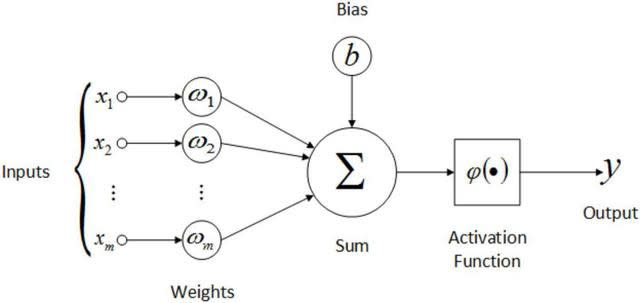
\includegraphics[width=0.6\columnwidth]{images/perceptron.jpeg}
    \caption{Illustration of a single leayer perceptron.}
    \label{fig:perceptron}
\end{figure}


\subsection{Perceptrons as Logical Operators}\label{Perceptrons-as-Logical-Operators}

\textbf{Motivation:} Showcasing the expressive power of neural networks.

\textbf{AND Perceptron:}
\begin{itemize}
  \item Set the bias $w_0 = -1.5$ and the weights $w_1 = w_2 = 1$
  \item Now the function $w_1x_1 + w_2x_2 + w_0 > 0$ if and only if $x_1 = x_2 = 1$
  \item The function is a hyperplane (line) that linearly separates the point (1, 1) from the other three possible input combinations
  \begin{figure}[H]
    \centering
      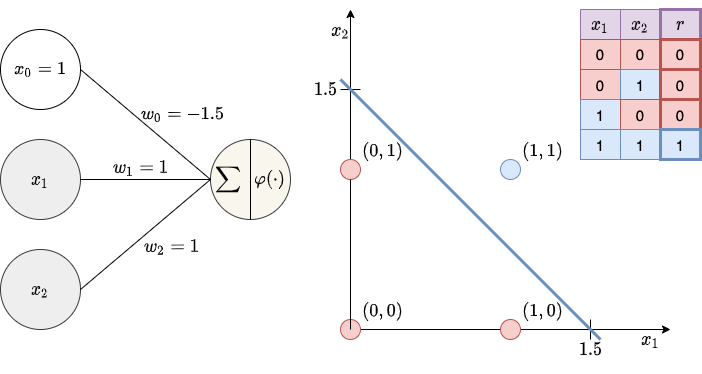
\includegraphics[width=0.9\columnwidth]{images/and-perceptron.png}
      \caption{Illustration of AND perceptron.}
      \label{fig:and-perceptron}
  \end{figure}
\end{itemize}

\textbf{OR Perceptron:}
\begin{itemize}
  \item Set the bias $w_0 = -0.5$ and the weights $w_1 = w_2 = 1$
  \item Now the function $w_1x_1 + w_2x_2 + w_0 > 0$ if and only if $x_1 = 1$ or $x_2 = 1$
  \item The function is a hyperplane separating the point (0, 0) from the other input combinations
  \begin{figure}[H]
    \centering
      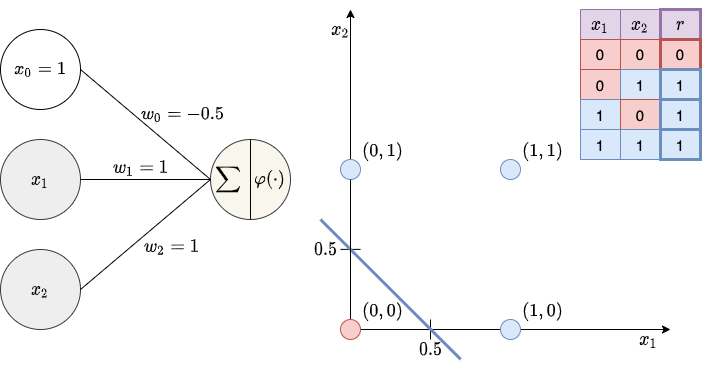
\includegraphics[width=0.9\columnwidth]{images/or-perceptron.png}
      \caption{Illustration of OR perceptron.}
      \label{fig:or-perceptron}
  \end{figure}
\end{itemize}

\textbf{XOR Multi-Layer Perceptron (MLP):} The exclusive OR, or XOR operator cannot be represented by a single-leyer perceptron, as XOR function is not linearly separable. XOR can be computed by a Multi-Layer Perceptron.
$$
XOR(x_1,x_2) = (x_1 \text{ AND NOT}(x_2)) \textbf{ OR } (\text{NOT}(x_1) \text{ AND } x_2)
$$
\begin{itemize}
  \item The first layer computes two hyperplanes:
  \begin{itemize}
    \item $z_1 = x_1 - x_2 - 0.5 > 0$ if and only if $(x_1 \text{ AND NOT}(x_2))$
    \item $z_2 = -x_1 + x_2 - 0.5 > 0$ if and only if $\text{NOT}(x_1) \text{ AND }(x_2))$
  \end{itemize}
  \item The second layer computes a single hyperplane implementing the OR $z_1 + z_2 - 0.5 > 0$ if and only if $z_1$ OR $z_2$ is true
  \begin{figure}[H]
    \centering
      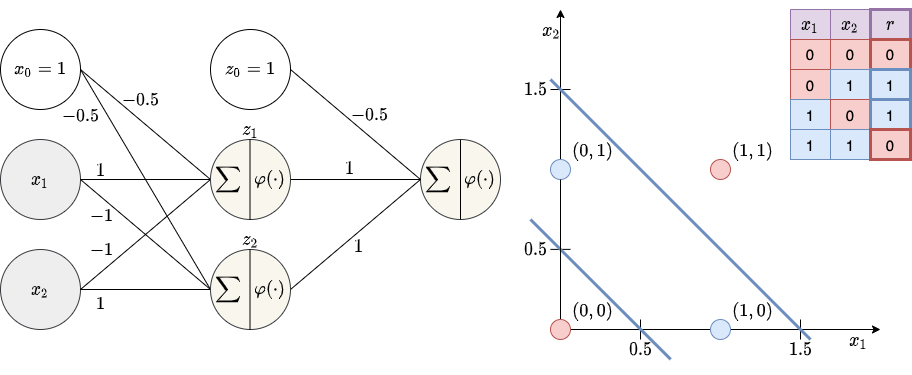
\includegraphics[width=0.9\columnwidth]{images/xor-perceptron.png}
      \caption{Illustration of XOR perceptron.}
      \label{fig:xor-perceptron}
  \end{figure}
\end{itemize}







\begin{center}\rule{3in}{0.4pt}\end{center}






















  \newpage
  \part{Additional learning models}
  \newpage









\section{Feature Engineering and Selection}\label{feature-engineering-and-selection}

\textbf{Why:} It can be argued that good data representation is actually more important than the choice of the learning algorithm.

\textbf{How:} There are variety of \textbf{\textcolor{blue}{feature engineering techniques}}:

\begin{itemize}
  \item \textbf{\textcolor{blue}{Feature transformation:}} convert the features in a form that allows learning better
  \item \textbf{\textcolor{blue}{Feature selection:}} aim to reduce the number of input variables that are used by the predictor
  \item \textbf{\textcolor{blue}{Feature generation:}} build new features by combining the original ones either manually (using prior knowledge) or by learning representations by optimizing some objective
\end{itemize}

\subsection{Feature transformation}\label{feature-transformation}

\textbf{Why:} to make the \uline{distribution of the input variables to better represent the domain knowledge} \textbf{or} to make the \uline{data more suitable to the learning algorithm}

\textbf{Objectives:} \uline{better error rates} \textbf{or} \uline{faster optimization}

\textbf{How:} Some \textbf{common \textcolor{blue}{feature transformations}:} (let $f=(f_1,...,f_m)$ denote the values of a single variable/feature in the dataset)
\begin{itemize}
  \item \textbf{\textcolor{blue}{Centering}:}
  \begin{gather*}
    f_i' = f_i - \bar{f} \\ \\
    \textbf{Where: } \textbf{$\bar{f}$: } \text{mean of variable}
  \end{gather*}
  \begin{itemize}
    \item \textbf{Rationale:} learning algorithms generally learn from the variance of the data, not the mean. Centering \uline{makes the variance more obvious}.
  \end{itemize}
  \item \textbf{\textcolor{blue}{Standardization (Z-score Normalization)}:}
  \begin{gather*}
    f_i' = \frac{f_i - \bar{f}}{\sqrt{\text{var}(f)}} \\ \\
    \textbf{Where: } \text{$\text{var}(f)$: } \text{variance of variable}
  \end{gather*}
  \begin{itemize}
    \item \textbf{Rationale:} making all variables have zero mean and unit variance may \uline{help if the raw variables have very different scales}.
  \end{itemize}
  \item \textbf{\textcolor{blue}{Unit range (min-max scaling)}:}
  \begin{gather*}
    f_i' = \frac{f_i - f_{min}}{f_{max}-f_{min}}
  \end{gather*}
  \begin{itemize}
    \item \textbf{Rationale:} unit range $[0,1]$ is useful \uline{if the variable's relative position in the observed range is important}.
  \end{itemize}
  \item \textbf{\textcolor{blue}{Clipping}:}
  \begin{gather*}
    f_i' = \text{sgn}(f_i) \text{min}(b, |f_i|) \text{, for some threshold } b > 0 \\ \\
    \textbf{Where: } \text{$\text{sgn}(f_i)$: } \text{sign function}
  \end{gather*}
  \begin{itemize}
    \item \textbf{Rationale:} \uline{if certain large values are known to be non-informative}, clipping may make learning easier (clipping small values: use max instead of min).
  \end{itemize}
  \item \textbf{\textcolor{blue}{Logarithmic transformation}:}
  \begin{gather*}
    f_i' = \text{log}(b + f_i) \text{, for some constant } b > 0
  \end{gather*}
  \begin{itemize}
    \item \textbf{Rationale:} log-transform can be used to \uline{emphasize small differences between small values} (e.g. 0 vs. 1) if they are more important than small differences between large values (e.g. 1000 vs. 1001).
  \end{itemize}
  \item \textbf{\textcolor{blue}{Sigmoid transformation}:}
  \begin{gather*}
    f_i' = \frac{1}{1 + \exp{(b f_i)}}
  \end{gather*}
  \begin{itemize}
    \item \textbf{Rationale:} Compresses the high absolute values heavily, \uline{"soft version" of clipping}.
  \end{itemize}
  \item \textbf{\textcolor{blue}{Normalization of feature vectors (Unit-Length Scaling)}:}
  \begin{gather*}
    x' = \frac{x}{||x||} \\ \\
    \textbf{Where: } \text{$x$: } \text{is the feature vector} \\
    ||x|| = \text{ Euclidean length of the feature vector}
  \end{gather*}
  \begin{itemize}
    \item \textbf{Rationale:} useful \uline{if the relative values of the variables for a single example are important rather than the absolute values}, e.g. if large object produces large average values for all features but the class of the object does not depend on its size.
  \end{itemize}
\end{itemize}

In general, \uline{several transformations are used to establish a desired effect}, e.g. log-transform + normalization








\subsection{Feature selection}\label{feature-selection}


\textbf{Why:} Potential benefits:
\begin{itemize}
  \item \textbf{Facilitating data visualization and \textcolor{Green}{interpretation}:} a model with fewer features is easier to explain
  \item \textbf{Reducing \textcolor{Green}{time and space} requirements of training models:} less data to store and compute over
  \item \textbf{Improving the \textcolor{Green}{predictive performance}:} a small subset of variables is less likely to overfit
\end{itemize}

\textbf{How:} \textcolor{blue}{Exhaustive search} approach goes through all $2^d - 1$ feature subsets and would give us the \textcolor{Green}{optimal feature subset}, however it is \textcolor{red}{prohibitively expensive} unless d (the set of features) is very small.

In general, \textbf{\textcolor{blue}{feature selection approaches}} aim to avoid the exponential complexity of checking each feature subset:

\begin{itemize}
  \item \textbf{\textcolor{blue}{Variable ranking ("filtering" approach)}:} assess the \uline{usefulness of each input feature individually} in a preprocessing step prior to learning, select a subset of most useful features
  \item \textbf{\textcolor{blue}{Variable subset selection}:} generate \uline{several different feature subsets} generally by some greedy search strategy, train a model with each subset, select the subset with the best predictive performance
  \item \textbf{\textcolor{blue}{Embedded methods}:} the learning algorithm \uline{performs variable selection}
\end{itemize}



\subsubsection{Variable ranking ("filtering" approach)}\label{variable-ranking}


\textbf{Pros and cons:}
\begin{itemize}
  \item[\textcolor{Green}{+}] reasonably efficient:
  \begin{itemize}
    \item computation of the \textbf{feature scores} can be done in $O(md)$ for correlation and $O(dm \log_2 m)$ time for the decision stump (the dominating cost is sorting the values of the feature $j$ in $O(m \log_2 m)$ time)
    \item The \textbf{ranking of the features} given the scores also requires sorting the features in $O(d \log d)$ time.
  \end{itemize}
  \item[\textcolor{red}{-}] limited by two issues:
  \begin{itemize}
    \item \textbf{Features} that are not correlating with the output \textbf{(not selected)} \textcolor{red}{may still be useful when combined by other variables}
    \item As the \textbf{filtering is made independently of the predictive model} that will use the selected features, the \textcolor{red}{selected subset might not be optimal}
  \end{itemize}
\end{itemize}

\textbf{A generic variable ranking procedure:}
\begin{itemize}
  \item Compute a score $s_j$ for each input variable $j$ using some \textbf{scoring criterion}
  \item Sort the variables in descending order of $s_j$
  \item Select a subset of the most highly ranking variables, e.g. by top $k$ variables or all variables exceeding a score threshold $\theta$ ($k$ or $\theta$ generally decided by the user)
\end{itemize}

\subsubsubsection{Regression-based scoring criterion : Pearson correlation}\label{regression-based-scoring-criterion}

\begin{itemize}
  \item Assume a dataset $S = \{(x_i,y_i)\}^m_{i=1}$, where $x_i = (x_{i1},...,x_{id})^T$, and $y_i \in R$
  \item (Empirical) Pearson correlation of the $j$'th feature and the output is given by
  \begin{gather*}
    r_j = \frac{\sum_{i=1}^m (x_{ij}-\bar{x}_j)(y_i-\bar{y})}{\sqrt{\sum_i (x_{ij}-\bar{x}_j)^2} \sqrt{\sum_i (y_i - \bar{y})^2}} \\ \\
    \textbf{Where: } \\
    \bar{x}_j = \frac{1}{m} \sum_{i=1}^m x_{ij} \text{ denotes the mean of the $j$'th feature in the dataset} \\
    \bar{y} = \frac{1}{m} \sum_{i=1}^m y_i \text{ denotes the mean of the output variable}
  \end{gather*}
  \begin{itemize}
    \item $r_j$ ranges from $+1$ (perfect correlation) to $-1$ (perfect anti-correlation)
    \item Pearson correlation has a natural interpretation in terms of linear regression. $r_j$ is the optimal regression co-efficient in a univariate linear model $y = rx + b$ that has the smallest mean squared error on the data
    $$
    r_j = \argmin_{r \in \mathbb{R}} \frac{1}{m} \sum_{i=1}^m (rx_{ij} + b - y_i)^2
    $$
  \end{itemize}
  \item For feature scoring, we use $s_j = r_j^2$ to allow selection of both anti-correlated and correlated features
  \begin{itemize}
    \item $r_j^2$ is the fraction of the variance of the output variable explained by the linear model
    \item $r_j^2 = 0$ means that the $j$'th feature alone does not explain any of the variance of the output
  \end{itemize}
\end{itemize}


\subsubsubsection{Classification-based scoring criterion}\label{classification-based-scoring-criterion}

\begin{itemize}
  \item Given $y \in \{-1, +1\}$, a simple approach of to consider a model
  $$
  y = \text{sgn}(ax + \theta)
  $$
  \begin{itemize}
    \item Where $a \in \{-1, +1\}$ and $\theta \in \mathbb{R}$ is set to optimize the empirical error
    $$
    [a_j, \theta_j] = \argmin_{a \in \{-1, +1\}, \theta \in \mathbb{R}} \sum_{i=1}^m 1_{\text{sgn}(ax_{ij}+\theta) \neq y_i}
    $$
  \end{itemize}
  \item For feature scoring, we can use the accuracy (or some other evaluation metrics for classification):
  $$
  r_j = 1 - \frac{1}{m} \sum_{i=1}^m 1_{\text{sgn}(ax_{ij}+\theta) \neq y_i}
  $$
\end{itemize}




\subsubsection{Variable subset selection}\label{variable-subset-selection}

\textbf{What (recap):} generate \uline{several different feature subsets} generally by some greedy search strategy, train a model with each subset, select the subset with the best predictive performance.

\subsubsubsection{Wrapper approach}\label{wrapper-approach}

\textbf{How:} The wrapper approach to variable selection \uline{uses the same learning algorithm that is used for the final model to evaluate variable subsets}
\begin{itemize}
  \item It iterates two steps:
  \begin{enumerate}
    \item Generate a variable subset (by some fixed procedure)
    \item Evaluate the subset by training a model with the subset
  \end{enumerate}
\end{itemize}

\textbf{\textcolor{blue}{Variable scoring} in wrapper approach:}
\begin{itemize}
  \item In a wrapper algorithm it is natural to use the \uline{risk of the hypothesis} (either on training or validation data) as the variable scoring criterion
  \item This involves training and testing a hypothesis for each variable subset considered
  \begin{itemize}
    \item[\textcolor{red}{-}] \textcolor{red}{Computationally heavier than the filter approach}
    \item[\textcolor{Green}{+}] But can find \textcolor{Green}{better variable subsets than the filter approach}
  \end{itemize}
\end{itemize}

\textbf{\textcolor{blue}{Two generic procedures} for generating a subset:}
\begin{itemize}
  \item \textbf{\textcolor{blue}{Forward selection}:} grow the set of selected variables by iteratively
  \item \textbf{\textcolor{blue}{Backward elimination}:} start from set of all variables and iteratively eliminate variables until a given stopping criterion is fulfilled
  \item Also more thorough search strategies can be used (best-first,
branch-and-bound, etc.)
\end{itemize}

\subsubsubsubsection{Greedy forward selection}\label{greedy-forward-selection}

\textbf{How:}
\begin{itemize}
  \item We \textbf{add a variables iteratively}, choosing in each step a \uline{variable that gives the maximum improvement}
  \item The variables that have been chosen to the model are not removed, even if they become redundant \textbf{(no back-tracking)}
  \item For each iteration, models are trained for every candidate variable to be added
  \item In total $O(Kd)$ models are trained where $K$ is the upper bound for the number of variables selected
\end{itemize}


\begin{tcolorbox}[title={Greedy forward selection pseudo-code}]

  \textbf{Input:} Dataset $S = \{(x_i,y_i)\}_{i=1}^m$

  \textbf{Input:} Maximum number of variables $K$

  \textbf{Initialize:} $J \leftarrow \emptyset, s_J \text{ (score)} \leftarrow 0; k \leftarrow 0$

  \textbf{Repeat:}
  \begin{description}
    \item $\;\;\;$ \textbf{for $j \in \{1,..., d\} \setminus J$} (all except the ones that are in $J$ already):
    \begin{description}
      \item $\;\;\;$ Train a model $f_{J \cup j}$ with input variable $J \cup j$
      \item $\;\;\;$ $s_{J \cup j} \leftarrow$ accuracy of the model $f_{J \cup j}$ (training set or validation set)
    \end{description}
    \item $\;\;\;$ Select the best variable: $j^* \leftarrow \argmax_{j \in \{1,..., d\} \setminus J} s_{J \cup j}$
    \item $\;\;\;$ \textbf{if $s_{J \cup j^*} > s_J$:}
    \begin{description}
      \item $\;\;\;$ $J \leftarrow J \cup j^*$
      \item $\;\;\;$ $k \leftarrow k+1$
    \end{description}
    \item $\;\;\;$ \textbf{else:}
    \begin{description}
      \item $\;\;\;$ stop $\leftarrow TRUE$
    \end{description}
    \item $\;\;\;$ \textbf{end if:}
    \begin{description}
      \item $\;\;\;$ $k = K$ or stop
    \end{description}
  \end{description}

  \textbf{Output:} A subset of selected variables $J \subset \{1,..., d\}$
\end{tcolorbox}



\subsubsubsubsection{Backward elimination}\label{backward-elimination}

\textbf{How:}
\begin{itemize}
  \item We \textbf{starts from the full set of input variables}
  \item In each stage, the input variable whose elimination has the best effect on the model is eliminated
  \begin{itemize}
    \item Largest increase or smallest decrease of accuracy on validation set
  \end{itemize}
  \item Accuracy on validation set generally used, since it will generally have an optimum for some number of selected variables
  \item In total $O(d^2)$ models are trained
\end{itemize}

\textbf{Why:} It is argued that backward elimination is \textcolor{Green}{more effective in finding good variable subsets than forward selection}


\begin{tcolorbox}[title={Backward elimination pseudo-code}]

  \textbf{Input:} Training set $S = \{(x_i,y_i)\}_{i=1}^m$

  \textbf{Input:} Validation set $V = \{(x_i,y_i)\}_{i=1}^n$

  \textbf{Initialize:} $J \leftarrow \{1,..., d\}, s_{\max} \text{ (score)} = 0; J_{\max} = J$

  \textbf{Repeat:}
  \begin{description}
    \item $\;\;\;$ \textbf{for $j \in J$:}
    \begin{description}
      \item $\;\;\;$ Train a model $f_{J \setminus j}$ with input variable excluding $j$
      \item $\;\;\;$ $s_{J \setminus j} \leftarrow$ accuracy of the model $f_{J \setminus j}$ on the validation set
    \end{description}
    \item $\;\;\;$ Variable whose elimination gives the best model: $j^* \leftarrow \argmax_{j \in J} s_{J \setminus j}$
    \item $\;\;\;$ $J \leftarrow J \setminus j^*$
    \item $\;\;\;$ Keep track of the best model:
    \item $\;\;\;$ \textbf{if $s_J > s_{\max}$:}
    \begin{description}
      \item $\;\;\;$ $s_{\max} = s_J$
      \item $\;\;\;$ $J_{\max} = J$
    \end{description}
    \item $\;\;\;$ \textbf{until $J = \emptyset$}
  \end{description}

  \textbf{Output:} A subset of selected variables $J_{\max} \subset \{1,..., d\}$
\end{tcolorbox}










\subsubsection{Embedded methods}\label{embedded-methods}

\textbf{How:} Embedded feature selection algorithms refer to cases where the learning algorithm itself is selecting features as part of searching for the best model

\begin{itemize}
  \item Models based on logical tests on single variable values e.g. decision trees
  \item Boosting algorithms using base hypotheses on single variables
  \item \textbf{\textcolor{blue}{Sparse modelling methods}:} focused on penalizing the weights with sparsity inducing norms
\end{itemize}


\subsubsubsection{Sparse modelling}\label{sparse-modelling}

\textbf{What:} Roughly speaking, a vector $x$ is \textbf{sparse} if it \uline{contains many zeros}.

\textbf{How:} $\ell_1$ norm $||x||_1$ promotes sparsity:

\begin{figure}[H]
  \centering  % Remember to centre the figure
    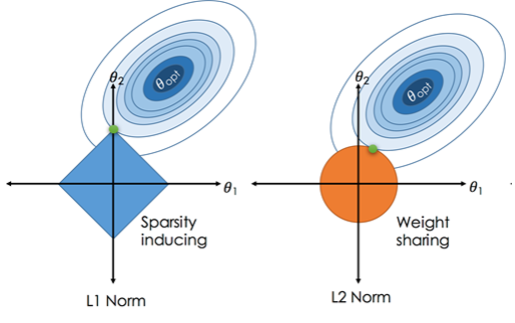
\includegraphics[width=0.8\columnwidth]{images/l1-sparsity.png}
    \caption{Visualizing the sparsity of L1 norm.}
    \label{fig:l1-sparsity}
\end{figure}



\textbf{Sparsity-inducing norms: $\ell_p$}

\begin{itemize}
  \item But is some other $p$ also possible?
  \item For general $p$, the $\ell_p$ norm is given by
  $$
  ||w||_p = (\sum_{j=1}^d |w_j|^p)^{1/p}
  $$
  \item For $p < 1$ the constraint region $||w||_p \leq 1$ becomes \textcolor{red}{non-convex} with ”spikes” extending towards the corners: will give sparsity but hard to optimize
  \item For $p > 1$ the the constraint region is more and more ”ball-like” and ”box-like” and will give \textcolor{red}{less and less sparsity}
  \item $p = 1$ gives the \textcolor{Green}{most sparse solutions} while keeping optimization problem \textcolor{Green}{convex}
  \begin{figure}[H]
    \centering  % Remember to centre the figure
      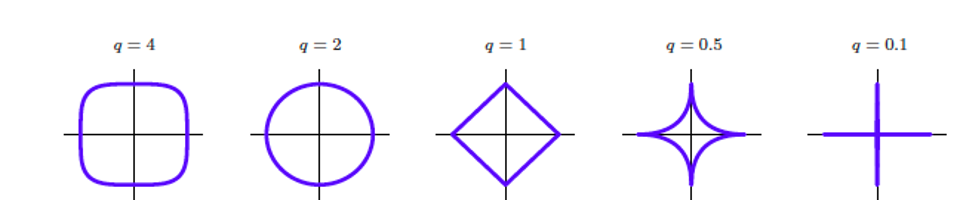
\includegraphics[width=1.0\columnwidth]{images/p-norms.png}
      \caption{Visualizing different norms.}
      \label{fig:p-norms}
  \end{figure}
\end{itemize}



\textbf{Sparse learning problems:}
\begin{itemize}
  \item Combining $\ell_1$ regularisation with different loss functions gives sparse variants of well-known models
  \begin{itemize}
    \item Squared loss $\Rightarrow$ Sparse regression, LASSO:
    $$
    \min_w \frac{1}{m} \sum^m_{i=1} L_{sq}(w^Tx_i, y_i) + \lambda ||w||_1
    $$
    \item Hinge loss $\Rightarrow$ Sparse SVM:
    $$
    \min_w \frac{1}{m} \sum^m_{i=1} L_{Hinge}(w^Tx_i, y_i) + \lambda ||w||_1
    $$
    \item Logistic loss $\Rightarrow$ Sparse logistic regression:
    $$
    \min_w \frac{1}{m} \sum^m_{i=1} L_{Logistic}(w^Tx_i, y_i) + \lambda ||w||_1
    $$
  \end{itemize}
\end{itemize}




\subsubsection{Stability of feature selection}\label{stability-of-feature-selection}

A recognized \textcolor{red}{problem} with \uline{variable subset selection} and \uline{sparse modelling} approaches is their \textcolor{red}{sensitivity to small perturbations}

\begin{itemize}
  \item upon \uline{removal or addition of a few variables} or examples
  \item \uline{addition of noise}
  \item \uline{initial conditions} of the algorithms
\end{itemize}

The \textcolor{red}{lack of stability} may sometimes be a \textcolor{red}{problem}

\begin{itemize}
  \item It may be a symptom of a ”bad” model, one that will \textcolor{red}{not generalize well}
  \item The results are \textcolor{red}{not reproducible}
  \item One \textcolor{red}{variable subset fails to capture the ”whole picture”}
\end{itemize}

A general approach to \textcolor{Green}{tackle the lack of stability} is to use \textbf{bootstrapping}
\begin{itemize}
  \item One runs the variable selection or sparse modelling algorithm on $T$ sub-samples, drawn with replacement from the original training data
  \item The \textbf{final variable subset} may be selected as
  \begin{itemize}
    \item The \uline{union of all selected features in the $T$ models}, or
    \item Counting how many models include a given variable $j$ and selecting the \uline{variables that occur at least given fraction of the $T$ models}
  \end{itemize}
\end{itemize}




\begin{center}\rule{3in}{0.4pt}\end{center}




















\section{Multi-class Classification}\label{multi-class-classification}

\textbf{What:} the problem of classifying instances into one of \uline{three or more classes}.


\textbf{How:}

\begin{itemize}
  \item Given a training dataset $\{(x_i,y_i)\}^m_{i=1},(x_i,y_i) \in \mathcal{X} \times \mathcal{Y}$
  \item Outputs belongs to a set of possible classes or labels: $$y_i \in \mathcal{Y} = \{1,2,...,k\}$$
  \item We aim learning a function $f: X \to \mathcal{Y}$
\end{itemize}

\textbf{multi-class classification vs. multi-label classification:}
\begin{itemize}
  \item In \textbf{multi-class classification}, \textcolor{blue}{one} of the labels is considered to be the \textcolor{blue}{correct label}, the other ones incorrect
  \item In \textbf{multi-label classification}, \textcolor{blue}{several of the labels can be correct} for a given input $x_i$, the output space will be $\mathcal{Y} = \{-1, +1\}^k$ , each output $y_i$ is a $k$-dimensional vector
\end{itemize}


\textbf{Two basic strategies to solve the problem:}

\begin{enumerate}
  \item \textbf{\textcolor{blue}{Aggregated methods using multiple binary classifiers}:}
  \begin{itemize}
    \item \textcolor{blue}{One-versus-all (OVA) approach}: Separate each class from all the others
    \item \textcolor{blue}{One-versus-one (OVO) or all-pairs approach}: Separate each class pair from each other
    \item \textcolor{blue}{Error-correcting output codes (ECOC) approach}: Represent each class with a binary code vector and predict the bits of the vector
  \end{itemize}
  \item  \textbf{\textcolor{blue}{Standalone models}: learning to predict multiple classes directly}
  \begin{itemize}
    \item Multiclass SVM
    \item Multiclass Boosting
  \end{itemize}
\end{enumerate}








\subsection{One-versus-All (OVA) Classification}\label{ova-classification}

\textbf{Pros and cons:}
\begin{itemize}
  \item[\textcolor{Green}{+}] \textcolor{Green}{Simple to implement} and thus popular
  \item[\textcolor{Green}{+}] \textcolor{Green}{Training is relatively efficient} with $O(kt)$ time where $t$ is the time to train a single binary classifier, if $k$ (\# of classes) is not too large
  \item[\textcolor{red}{-}] May suffer from \textcolor{red}{class imbalance} of the training sets for a given class $\ell$: there may be a low number of positive examples and a high number of negative examples per class
  \item[\textcolor{red}{-}] In general suffers from a \textcolor{red}{calibration problem}: the scores $f_{\ell}(x)$ returned by the individual classifiers may not be comparable
  \item[\textcolor{red}{-}] \textcolor{red}{Doesn't always produce the optimal empirical error rate} for the dataset
\end{itemize}


\textbf{How:}

\begin{itemize}
  \item Given a training dataset $\{(x_i,y_i)\}^m_{i=1},(x_i,y_i) \in \mathcal{X} \times \mathcal{Y}$
  \item If we have $k > 2$ classes we will train $k$ binary hypotheses $h_1, ..., h_k; \\ h_{\ell} : X \to \{+1,-1\}$
  \item For training the $\ell$th hypothesis, new binary labels, called the \textbf{surrogate labels} are computed
  $$
  \tilde{y}_i^{(\ell)} =
  \begin{cases}
	+1, & \text{if $y_i = \ell$} \\
  -1, & \text{if $y_i \neq \ell$}
	\end{cases}
  $$
  \item A binary classifier is trained to predict the surrogate labels
  \item The hypothesis class for the binary classifiers is not restricted: we can use any that is deemed suitable
\end{itemize}


\textbf{OVA prediction:}

\begin{itemize}
  \item In general, there may be more than one class $\ell$ for which $h_{\ell}(x) = +1$
  \begin{itemize}
    \item Some \textcolor{red}{arbitrary tie-breaking} could be used, e.g. predict the class with the smallest index $\ell$
    \item Better results can be obtained if the hypotheses also provide some \textcolor{Green}{real-valued score $f_{\ell}(x) \in \mathbb{R}$ (confidence, margin, etc.)} for the label to be $\ell$.
  \end{itemize}
  \item In that case, we can choose the label with the highest score
  $$
  h(x) = \argmax_{\ell} f_{\ell}(x)
  $$
  \begin{itemize}
    \item E.g. with linear models $h_{\ell}(x) = \text{sgn}(w_{\ell}^T x)$ using the margin of the example is a natural choice $f_{\ell}(x) = w_{\ell}^T x$
  \end{itemize}
\end{itemize}



\begin{tcolorbox}[title={OVA training pseudo-code}]

  \textbf{Input:} Training set $S = \{(x_i,y_i)\}_{i=1}^m, x_i \in X, y_i \in \mathcal{Y} = {1, ..., k}$

  \textbf{for $\ell \in \{1, ..., k\}$:}
  \begin{description}
    \item $\;\;\;$ Generate training dataset with surrogate labels: $\{(x_i, \tilde{y}_i^{(\ell)})\}_{i=1}^m$
    \item $\;\;\;$ Train a binary hypothesis $h_{\ell} : X \to \{-1,+1\}$
    \item $\;\;\;$ Let $f_{\ell}(x)$ be the score for $x$ given by the model $h_{\ell}$
  \end{description}
  $h(x) = \argmax_{\ell} f_{\ell}(x)$

  \textbf{Output:} Multiclass hypothesis $h: X \to \mathcal{Y}$
\end{tcolorbox}






\subsection{One-versus-One (OVO) (a.k.a all-pairs) Classification}\label{ovo-classification}


\textbf{Pros and cons:}
\begin{itemize}
  \item[\textcolor{red}{-}] Compared to OVA, we are training many \textcolor{red}{more binary classifiers}: $O(k^2)$ compared to $O(k)$
  \item[\textcolor{Green}{+}/\textcolor{red}{-}] However, the \textbf{training sets are smaller} since they only contain examples of two classes at a time:
  \begin{itemize}
    \item[\textcolor{Green}{+}] \textcolor{Green}{Faster to train}
    \item[\textcolor{Green}{+}] The OVO \textcolor{Green}{training sets are less likely to be imbalanced} than in OVA
    \item[\textcolor{red}{-}] \textcolor{red}{Increased chance of overfitting} (due to smaller training set)
  \end{itemize}
  \item[\textcolor{Green}{+}] \textcolor{Green}{Better theoretical justification} (compared to OVA) through the \textbf{majority voting ensemble} approach
\end{itemize}



\textbf{How:}

\begin{itemize}
  \item In OVO classification, we divide a multiclass problem into a set of $k(k - 1)/2$ binary classification problems, one for each pair of classes $(\ell,\ell'),1 \leq \ell < \ell ' \leq k$
  \item FThis entails generating a new training set consisting of examples of the pair of classes $(\ell,\ell')$ and generating a \textbf{surrogate labels}
  $$
  \tilde{y}^{\ell, \ell'} =
  \begin{cases}
	+1, & \text{if $y = \ell$} \\
  -1, & \text{if $y = \ell'$}
	\end{cases}
  $$
  \item For each class pair, a binary hypothesis $h_{\ell,\ell'}(x) : X \to \{-1, +1\}$ is trained using the generated training set
\end{itemize}



\textbf{OVO prediction:}

\begin{itemize}
  \item In predicting, for each class $\ell$ we have $k - 1$ pairwise hypotheses, one for each class containing $\ell$ $(h_{\ell,\ell'} \text{ and } h_{\ell',\ell}, \text{ for all } \ell' \neq \ell)$
  \item In the \textbf{ideal case}, all of the $k - 1$ hypotheses involving class $\ell$ would predict class
  \item \textbf{In practice} this may not happen, we might have for some classes $\ell', \ell''$
  \begin{itemize}
    \item $h_{\ell,\ell'} = +1$, predicting class $\ell$ for $x$
    \item $h_{\ell,\ell''} = -1$, predicting class $\ell''$ for $x$
  \end{itemize}
  \item We need to \uline{resolve these discrepancies}. A \textbf{voting approach} can be used:
  \begin{itemize}
    \item We count for each input $x$, how many pairwise hypotheses predict class $\ell$ (the votes)
    $$
    h(x) = \argmax_{\ell} \sum_{\ell < \ell'} 1_{\{h_{\ell\ell'}(x)=+1\}} + \sum_{\ell > \ell'} 1_{\{h_{\ell'\ell}(x)=-1\}}
    $$
    \item Ties can occur with several classes receiving the same number of votes, we can break them arbitrarily (e.g. predicting the smallest index $\ell$)
  \end{itemize}
\end{itemize}






\subsection{Error-correcting codes (ECOC) Classification}\label{ecoc-classification}

\textbf{What:} a general methods for reducing \textit{multi-class problems} \textbf{to} \uline{binary classification}

\textbf{How:}
\begin{itemize}
  \item Each class $\ell$ is allocated a codeword $m_\ell$ of length $c > 1$. In the simplest case a binary vector can be used $m_\ell \in \{-1, +1\}^c$.
  \item The code words of all $k$ classes together form a matrix $M \in \{-1,+1\}^{k \times c}$
  \begin{figure}[H]
    \centering  % Remember to centre the figure
      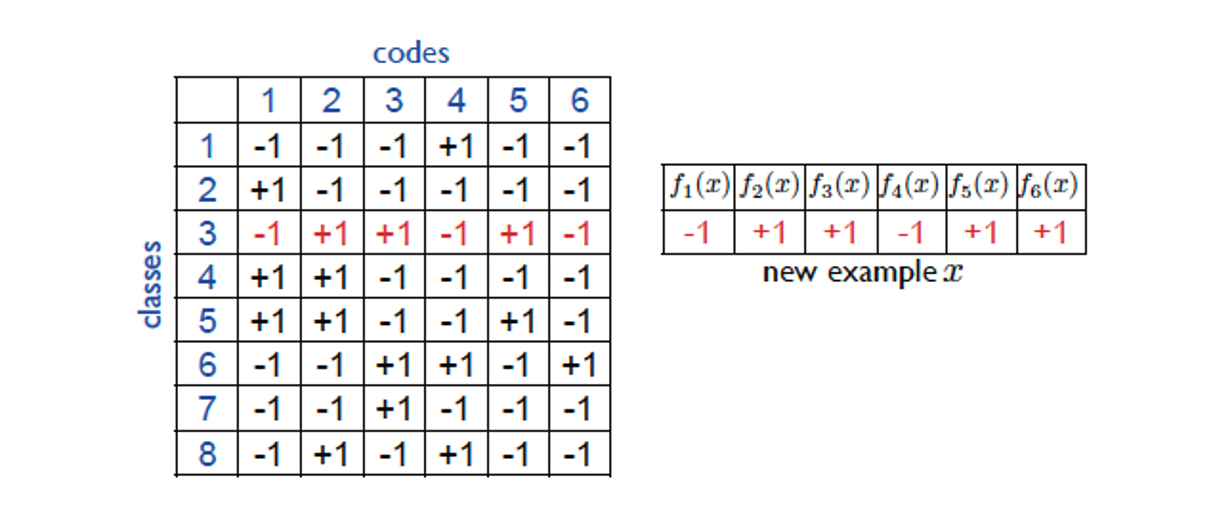
\includegraphics[width=1.0\columnwidth]{images/ecoc.png}
      \caption{Illustration of matrix $M$ in the ECOC approach.}
      \label{fig:ecoc}
  \end{figure}
  \item Given the codeword matrix, a \textbf{binary classifier $f_j : X \to \{-1, +1\}$} is learned \uline{for each column $j = 1, ..., c$} of the codeword matrix
  \item The training data for the classifier of column j is relabeled with \textbf{surrogate labels}
  $$
  \tilde{y}_i^{(j)} =
  \begin{cases}
	m_{\ell,j}, & \text{if $y_i = \ell$} \\
  -m_{\ell,j}, & \text{if $y_i \neq \ell$}
	\end{cases}
  $$
  \item The \textbf{prediction} of the ECOC model is taken as the \uline{class $\ell$ with the fewest wrongly predicted columns of the keyword}:
  $$
  h(x) = \argmin_{\ell = 1}^k \sum_{j=1}^c 1_{f_j(x) \neq m_{\ell j}}
  $$
\end{itemize}


\textbf{How to generate the codewords?}

\begin{itemize}
  \item \textbf{Deterministic code:} decide on the length $c$ and choose binary vectors for each class so that the \uline{between class Hamming distance is as large as possible}
  \item \textbf{Random code:} draw code words \uline{randomly}
  \item \textbf{Use domain knowledge:} each \uline{column could be a feature describing the class}
\end{itemize}


\textbf{Why does ECOC work?}

\begin{itemize}
  \item The \textbf{prediction of the ECOC model} can be seen as \uline{correcting incorrectly predicted bits of the codeword}
  \begin{itemize}
    \item corrected codeword = the one in the codebook (matrix $M$) that has the smallest Hamming distance to the predicted codeword
    \item If the between class Hamming distance of the codewords is at least $d$, the upto $\frac{d-1}{2}$ one bit errors can be corrected
  \end{itemize}
  \item Another explanation comes from \textbf{ensemble learning:} \uline{model averaging between diverse classifiers $f_j$ happens by minimizing the Hamming distance between codewords}
\end{itemize}






\subsection{Standalone multi-class classifiers}\label{standalone-multiclass-classifiers}

\textbf{What:} Models that directly aim to minimize a multi-class loss function.

\textbf{Why:} \uline{May give better predictive performance} than the approaches based on aggregating binary classifiers. Also defining a combined model \uline{may be more efficient to train}.

\textbf{How:} Using models like Multiclass SVM, Multiclass boosting, Multiclass neural networks, Multiclass Decision trees and so on.



\subsubsection{Multi-class SVM}\label{multiclass-SVM}


\textbf{How:}

\begin{itemize}
  \item Multi-class SVM learns $k$ hyperplanes $f_{\ell}(x) = w_{\ell}^T x = 0$ simultaneously
  \item The \textbf{predicted class} is the class with the \uline{highest score}
  $$
  h(x) = \argmax_{\ell} f_{\ell}(x)
  $$
  \item The \textbf{objective} is to have the score of the correct class to be higher than all the other classes by a margin (of 1)
  $$
  w_{y_i}^T x_i - w_{\ell}^T x_i \geq 1 - \xi_i \text{, for all } \ell \neq y_i
  $$
  \begin{itemize}
    \item Above, slack $\xi_i \geq 0$ in used in the analogous way to binary SVMs to allow some examples to not to have the required margin
  \end{itemize}
\end{itemize}

\bigskip

Multi-class SVM has $k$ weight vectors $w_1 ,... , w_k$ to control
\begin{itemize}
  \item This is achieved by a regularizer that computes the sum of norms:
  $$
  \sum_{\ell=1}^k ||w||_2^2
  $$
  \item The regularizer is motivated by controlling the empirical Rademacher complexity $\hat{R}(H)$ of the hypothesis class $H$ of multi-class SVMs:
  $$
  \hat{R}(H) \leq \sqrt{\frac{r^2 \wedge^2}{m}}
  $$
  \begin{itemize}
    \item Where $\sum_{\ell=1}^k ||w_\ell||_2^2 \leq \wedge^2$ and $||x_i||_2^2 \leq r^2$ for all $i=1,...,m$
  \end{itemize}
  \item Thus, minimizing the sum of norms aids achieving good generalization
\end{itemize}


We can write the Multi-class SVM as regularized loss minimization problem. The Multi-class SVM optimization problem can be written as follows:

$$
\begin{aligned}
\min_{w,\xi} \quad & \underbrace{\frac{\delta}{2} \sum_{\ell=1}^{k} ||w_\ell||_2^2}_\text{Regularization} + \underbrace{\sum_{i=1}^m \max{\{0, 1-[w_{y_i}^T x_i - \max_{\ell \neq y_i} w_\ell^T x_i]\}}}_\text{multi-class Hinge loss}
\end{aligned}
$$

\begin{itemize}
  \item This problem corresponds to the QP formulation by setting $\lambda = 1/C$
  \item The problem is \textcolor{Green}{convex} but but the loss is piecewise linear, thus \textcolor{red}{not differentiable everywhere} $\rightarrow$ A \textbf{stochastic gradient descent} algorithm can be defined through computing the subgradients of the objective function
\end{itemize}



\textbf{Multi-class SVM with kernels:}

\begin{itemize}
  \item We can perform non-linear multi-class classification by using a kernel $\kappa(x, x') = \langle\phi(x), \phi(x')\rangle$ over the data
  \item The kernelized version of the multi-class SVM optimizes dual variables $\alpha = (\alpha_i,\ell), i = 1,...,m, \ell = 1,...,k$ (one dual variable for each training example $i$ and possible class $\ell$)
  \item The optimization problem is given by
  $$
  \begin{aligned}
  \max \quad & \sum_{i=1}^m \alpha_i,_{y_i} - \frac{1}{2} \sum_{\ell=1}^k \sum_{i,i'=1}^m \alpha_i,_\ell \alpha_{i'},_\ell \kappa(x_i, x_{i'}) \\
  \textrm{s.t.} \quad & \sum_\ell \alpha_i,_\ell = 0 \\
    & \alpha_i,_\ell \leq 0 \text{, for } \ell \neq y_i, 0 \leq \alpha_i,_{y_i} \leq C \\
  \end{aligned}
  $$
  \item Model's prediction in dual form:
  $$
  \hat{y}(x) = \argmax_{\ell = 1,...,k} \sum_{i=1}^m \alpha_i,_\ell \kappa(x_i,x)
  $$
\end{itemize}












\end{document}
